% center for academic English may have good resources
% font should 12pt -> 11pt
\documentclass[a4paper, twoside, 12pt]{report}

% Extra maths symbols (nexists)
\usepackage{amssymb}


\usepackage[dvipsnames]{xcolor}

%% Language and font encodings
\usepackage[english]{babel}
\usepackage[utf8]{inputenc}
\usepackage[T1]{fontenc}

%% Sets page size and margins
\usepackage[a4paper,top=3cm,bottom=2cm,left=3cm,right=3cm,marginparwidth=1.75cm]{geometry}

%% Useful packages
\usepackage{amsmath}
\usepackage{graphicx}
\usepackage[colorinlistoftodos]{todonotes}
\usepackage[colorlinks=true, allcolors=blue]{hyperref}

% Allow landscape
\usepackage{pdflscape}

% Controls spacing
\usepackage{parskip}

% verbatim with maths (lstlisting)
\usepackage{listings}
\lstset{
  basicstyle=\ttfamily,
  mathescape,
  breaklines=true,
  columns=flexible,
}


% Table column centering
\usepackage{array}
\newcolumntype{P}[1]{>{\centering\arraybackslash}p{#1}}
\newcolumntype{M}[1]{>{\centering\arraybackslash}m{#1}}

% For references
\usepackage[backend=biber]{biblatex}
\addbibresource{bibs/export.bib}

% Example numbering
\usepackage{amsthm}

% Enumerate examples
\theoremstyle{definition} % Use normal font for examples
\newtheorem{example}{Example}


\title{Automatic Concept Extraction and Its Use in Explaining Video Classification}
\author{Roko Parać}
% Update supervisor and other title stuff in title/title.tex

\begin{document}
\renewcommand{\vec}[1]{\textbf{#1}}
\newcommand{\curly}[1]{\mathcal{#1}}
\newcommand{\expct}{\mathbb{E}}
\newcommand{\reals}{\mathbb{R}}


\begin{titlepage}

\newcommand{\HRule}{\rule{\linewidth}{0.5mm}} % Defines a new command for the horizontal lines, change thickness here

%----------------------------------------------------------------------------------------
%	LOGO SECTION
%----------------------------------------------------------------------------------------


\includegraphics[width=8cm]{title/logo.eps}\\[1cm] % Include a department/university logo - this will require the graphicx package
 
%----------------------------------------------------------------------------------------

\center % Center everything on the page

%----------------------------------------------------------------------------------------
%	HEADING SECTIONS
%----------------------------------------------------------------------------------------

\textsc{\LARGE MEng Individual Project}\\[1.5cm] % Name of your university/college
\textsc{\Large Imperial College London}\\[0.5cm] % Major heading such as course name
\textsc{\large Department of Computing}\\[0.5cm] % Minor heading such as course title

%----------------------------------------------------------------------------------------
%	TITLE SECTION
%----------------------------------------------------------------------------------------
\makeatletter
\HRule \\[0.4cm]
{ \huge \bfseries \@title}\\[0.4cm] % Title of your document
\HRule \\[1.5cm]
 
%----------------------------------------------------------------------------------------
%	AUTHOR SECTION
%----------------------------------------------------------------------------------------

\begin{minipage}{0.4\textwidth}
\begin{flushleft} \large
\emph{Author:}\\
\@author % Your name
\end{flushleft}
\end{minipage}
~
\begin{minipage}{0.4\textwidth}
\begin{flushright} \large
\emph{Supervisors:} \\
Dr. Alessandra Russo 

Dr. Luke Dickens \\[1.2em] % Supervisor's Name
\emph{Second Marker:} \\
Dr. Robert Chatley % second marker's name
\end{flushright}
\end{minipage}\\[2cm]
\makeatother

% If you don't want a supervisor, uncomment the two lines below and remove the section above
%\Large \emph{Author:}\\
%John \textsc{Smith}\\[3cm] % Your name

%----------------------------------------------------------------------------------------
%	DATE SECTION
%----------------------------------------------------------------------------------------

{\large \today}\\[2cm] % Date, change the \today to a set date if you want to be precise

\vfill % Fill the rest of the page with whitespace

\end{titlepage}

% Condensed version of the introduction
% Needs to answer questions: Why? What? How? What are the outcomes?

\begin{abstract}

The abstract will go here
\end{abstract}

\renewcommand{\abstractname}{Acknowledgements}
\begin{abstract}
The acknowledgements will go here
\end{abstract}


\tableofcontents
% \listoffigures
% \listoftables

\chapter{Introduction}

Natural language can be used as metadata for any sort of data.
To make it machine-readable and valuable for a task at hand, one needs to extract relevant pieces of information about it consistently.
If done successfully, given natural language explanations could even be used to explain unseen classification examples or improve the video classification performance.
In this project, a method for the automatic extraction of valuable information from language is studied as part of a bottleneck-based video classification pipeline.





\section{Problem Setup}

The project aims to design a general method for extracting valuable information from natural language.
The initial attempt at designing such a method intends to tackle a specific problem well before expanding its domain.
The problem this work is helping to solve is the problem of the classification of short baseball video sequences.
% TODO fix
In particular, it targets the MLB-V2E dataset  \cite{RefWorks:RefID:16-2021automatic}.
This dataset consists of the following:

 - A short video of a baseball sequence (\href{www.mlb.com}{MLB} (Major League Baseball) clips).
 
 - Label describing the outcome which occurred in it: strike, foul, ball, none, out.

 - Crowd-sourced brief explanation of why the outcome occurred.
 
 
\begin{center}
\begin{tabular}{ |p{1.5cm}|p{1.5cm}|p{9cm}|p{1.7cm}|  }
 \hline
 \multicolumn{4}{|c|}{Extract from MLB-V2E dataset} \\
 \hline
 id, $n$ & label, $l_n$ & explanation, $e_n$& video, $v_n$\\
 \hline
 1 & strike & The batter did not swing. The ball was in the strike zone. & N/A \\
 2 & foul & the batter hit the ball into the stands and it landed in foul territory & N/A \\
 3 & ball & The hitter didn’t swing. The ball was outside the strike zone. & N/A \\
 4 & none & The video did not load. & N/A \\
 5 & out & the batter hit the ball and it was caught by the fielder & N/A \\
 
 \hline
\end{tabular}
\end{center}


% TODO insert reference to the classifier %
Additionally, the problem is explored within the context of a concept bottleneck classifier. 
In that context, \textbf{concepts} are defined as syntactic generalisations of atomic sentences. 
Moreover, an \textbf{atomic sentence} is a sentence that an NLP expert cannot decompose into multiple sentences.
The system designed in this project should be general-purpose; changing the dataset on which the concept bottleneck classifier operates should immediately produce relevant concept sentences for a different dataset.

As such, this project aims to propose a novel method, combining techniques from natural language processing, deep learning and logic-based learning, that would extract domain-independent concept sentences.


\section{Limitations and Assumptions}
% Probably talk about in the initial project things.

At the moment, only the syntactic concept generalisation is being made. 
A consequence of using syntactic concept generalisation is that the events happening in the video are isolated as sentences with no content linking between them. 
Additionally, the tokens in a generalised concept sentence must first occur in the original one.
This procedure may result in grammatically incorrect sentences.
For example, consider a sentence: \emph{The left fielder caught the ball.}.
With our current approach, the system can extract the following sentence \emph{The fielder caught the ball.}.
However, the issue is that it can be unclear who \emph{the fielder} is now because it was previously determined by the adjective \emph{left}.

An extension might be able to relax this limitation.
The most straightforward possible approach for resolving this issue may replace \emph{the} with \emph{a} in a generalisation where additional information about the determined noun is removed.

More advanced generalisation could involve swapping words out for their synonyms.
An additional extension could involve linking entities from one sentence to another. 



\section{Objectives}

The objectives of this project are:

 - Develop and evaluate a general syntactic framework for extracting concept sentences from any given sentence. The process would be split into decomposing non-atomic sentences into atomic and generating concept sentences from atomic sentences.
 
 - Explore how does this framework aid deep neural network models in the context of video classification, namely whether an improvement is achieved for the MLB-V2E dataset \cite{RefWorks:RefID:16-2021automatic}.


 - Time permitting, generate a natural language explanation of the label chosen by the classifier. 


\section{Challenges}

This section highlights challenges that are anticipated to happen and a brief overview of its difficulties.
The section will be revised upon completion of the project once the topics' complexity is more evident.

The following questions will be difficult but necessary to answer as a part of this project:

 - \emph{How should a concept extracted from natural language be defined?} Making a helpful concept and immediately extensible to other domains may be difficult. One cannot use expert knowledge to help craft features that the subsequent architecture should use.
 
 
 - \emph{How will the concept extraction pipeline be scaled with a large amount of data?} The proposed system will include logic-based learning systems ILASP \cite{RefWorks:RefID:18-law2020ilasp} to extract syntactic concept sentences. 
 Unfortunately, the system is not scalable with respect to hypothesis space. On the other hand, more scalable alternative FastLAS \cite{RefWorks:RefID:19-law2020fastlas:} includes limitations that may be impossible to workaround.
 
 - \emph{How is an atomic sentence decomposed into a concept sentence?} This is the critical problem the system must resolve to be used.

 - \emph{How should the sentences be decomposed into atomic sentences?} This is one of the critical problems this system would need to resolve to be applied effectively. It may become a much more complex issue than concept sentence extraction, which can be designed as graph pruning of a dependency graph.
 


\section{Contributions}

Not relevant yet.

% What is the problem?
% Why is it interesting?
% What is the main idea for solving it?


\chapter{Background}

\section{Answer Set Programming}

Answer Set Programming  \cite{RefWorks:RefID:1-lifschitz2008answer} is a form of declarative programming, with a Prolog-like syntax suitable for solving NP-hard search problems.
However, it is based on a different computation mechanism than Prolog: stable model semantics \cite{RefWorks:RefID:21-fitting1992michael}.
Answer set solver is a program that generates stable models of an answer set program, which are solutions of an answer set program. 
The chosen answer set solver used throughout this project is clingo \cite{RefWorks:RefID:22-clingo}.

This section will briefly highlight the syntax of the answer set programs and the stable model semantics.

\subsection{Syntax}

Here are the types of rules in ASP\footnote{Disjunctive rules also exist, but they are omitted as they are not used in this work.}: 

 1. \emph{normal rule} -> $ h\; :- b_1, b_2, ..., b_n, not\; n_1, not\; n_2, ..., not\; n_o$
 
 2. \emph{hard constraint} -> $:- \; b_1, ..., b_n, not\; n_1, not\; n_2, ..., not\; n_o$
 
 3. \emph{choice rule} -> $lb\{h_1; ..., h_m\}ub\; :- \;  b_1, b_2, ..., b_n, not\; n_1, not\; n_2, ..., not\; n_o$
 
where $lb, ub$ are integers, $n_1,...,n_o$ are atoms and $b_1, ...,b_n$ are either atoms or aggregates.

Aggregates have the following syntax $lb\#agg\{e_1; ...; e_n\}ub$ where $lb, ub$ are ints, $agg$ is an aggregate function (e.g. $sum$) and $e_i$ is an aggregate element.
Additionally, aggregate element has the form  $t_1, ..., t_k : c_1, ..., c_j$ where $t_i$ is a term and $c_i$ is a literal.
 
This syntax is quite expressive. For instance, here are two ways to define a coin falling either on heads or tails.

\subsubsection{Method 1:}
\begin{verbatim}
coin(c1).
heads(C) :- coin(C), not tails(C).
tails(C) :- coin(C), not heads(C).
\end{verbatim}
\subsubsection{Method 2:}
\begin{verbatim}
coin(c1).
1 { heads(C); tails(C) } 1 :- coin(C).
\end{verbatim}

The results of these programs, i.e. the answer sets of the programs, are \{coin(c1), heads(c1)\} and \{coin(c1), tails(c1)\}.
It will be explained how they are computed in the subsequent subsection.

As seen in the example, a program can have multiple answer sets.
So, an additional piece of syntax is defined which evaluates whether some answer set is better than another.
This piece of syntax is referred to as a weak constraint.
It is of the form $:\sim {} b_1,..., b_n.[wt@lev, t1, ..., t_m]$
where $lev$ is an integer, $b_i$ a literal, and $t_i$ term.

\subsection{Semantics}

The Answer Set Programming is based on stable model semantics \cite{RefWorks:RefID:21-fitting1992michael}.

The answer set is defined as follows: 
\emph{Given a program P and a Herbrand interpretation X, X is an \textbf{answer set} of P iff X is a minimal Herbrand model of $RG(P)^X$ (reduct with respect to X).}

To understand the presented definition, one needs to know a few other concepts presented in this subsection.
Here the definitions for those concepts will mainly be explained intuitively rather than formally; for deeper understanding and more formal definitions, please refer to the \emph{Answer Set Programming} book \cite{RefWorks:RefID:23-lifschitz2019answer}. \\

\textbf{Herbrand interpretation} a program is an assignment of every element of the Herbrand base of that program to either true or false. \textbf{Herbrand base} of a program P is a set of all ground atoms that can be made using constants, predicate symbols, and functions of a program P.\\

When a Herbrand interpretation X satisfies all the rules in of a program, X is the \textbf{Herbrand model} of a program. X is also a minimal Herbrand model if there is no smaller subset X', also a Herbrand model.\\

\textbf{Relevant grounding} replaces variables with a program with constants available.
It iteratively fills up the rules by adding every rule whose elements of $body^+$(R) are heads of already included rules. 
The $body^+$ constraint ignores the $not$ atoms. 
For example, take P = \{p(X) :- q(X). q(a).\}. 
The first iteration of relevant grounding would create P' = \{q(a).\} while after the second one P' = \{q(a). p(a) :- q(a).\}\\

The \textbf{reduct of a program} P with respect to X ($P^X$) is a construct used to remove the $not\: c$ terms from a program.
Computing the reduct is done in the following manner. The solver assumes the X is a solution and iterates through every $not\: c$ within P. 
If $c$ is not in X (assumed to be false), then the $not\: c$ term is removed from the rule containing it. 
It essentially removes the need to worry about $not\: c$ since that term is satisfied.
On the other hand, if $c$ is in X, then the entire rule containing $not\: c$ is removed.
There is no need to consider the rule whose body is false since it cannot be satisfied.

Constructing the reduct of a \textbf{choice rule} has an additional step.
It is turned into either normal rules or a constraint.
Given a possible interpretation $X$, the choice rule $lb\{h_1; ..., h_m\}ub\; :- \;  b_1, b_2, ..., b_n, not\; n_1, ..., not\; n_o$ is converted in a following manner:

1. if $ lb \leq |\{h_1; ...; h_m\} \cap X| \leq ub$ then $h_i :- \;  b_1, b_2, ..., b_n, not\; n_1, ..., not\; n_o$ for is created for each $i \in \{1..m\}$

2. Otherwise, a constraint of the form $ :- \;  b_1, b_2, ..., b_n, not\; n_1, not\; n_2, ..., not\; n_o$ 
is created.\\

So, to check whether X is an answer set, one needs to compute a relevant grounding of a program. Then it needs to construct a reduct of that program with respect to X.
From the reduct, one can easily construct a minimal model M by starting from facts and iteratively adding heads of those rules with all body elements already in M.
Finally, if X = M, then X is an answer set.
Note that the head of a \textbf{constraint} is considered to be $\bot$. 
Hence, if the body of a constraint is satisfied, $\bot$ is added to M, so it cannot be equal to X.
In this manner, the constraints eliminate possible answer sets.






% Introduction to stable model semantics and its benefits over other forms of programming.
% Touch upon non-monotonicity. Its non-Turing completeness.

\section{Inductive Logic Programming}

% What is Inductive Logic Programming
Inductive Logic Programming \cite{RefWorks:RefID:42-muggleton1991inductive} is a field at an intersection of machine learning and logic programming.
In most cases, the goal of an inductive learning task is to learn a set of rules (a hypothesis H), which combined with the background knowledge B can entail every positive example while not entailing any negative example. 
Some systems use a weakened version of that statement to allow for noisy examples, such as the newer versions of ILASP \cite{RefWorks:RefID:55-law2018inductive}.

Many ILP systems have been developed over the years, such as Progol5 \cite{RefWorks:RefID:43-muggleton2000theory}, HAIL \cite{RefWorks:RefID:44-ray2003hybrid}, TopLog \cite{RefWorks:RefID:45-muggletontoplog:}, and TAL \cite{RefWorks:RefID:46-corapi2010inductive}.

The chosen system for this project is ILASP \cite{RefWorks:RefID:18-law2020ilasp}, a system that does the inductive learning of the answer sets programs.
Choosing a system that learns ASP is done because the ASP environment can effectively perform non-monotonic reasoning.\\

To understand the ILASP system fully, a few more definitions need to be introduced.

An atom A is \textbf{bravely entailed} if by a logic program P if it is included (true) in at least one answer set of P. 
On the other hand, an atom A is \textbf{cautiously entailed} if it is included (true) in all answer sets of P.

A pair $E = <E^{inc}, E^{exc}>$ (<inclusions, exclusions>) is a partial interpretation of sets of literals.
Answer set X extends E iff set of inclusions is a subset of X ($E^{inc} \subseteq X$) and X is disjoint with exclusions ($E^{exc} \cap A = \emptyset$).


The \textbf{language(inductive) bias} M, is a a pair $<M_h, M_b>$ which is used to construct the \textbf{search space} $S_M$ of a learning task.
The rule of the form  \\$ h \;{:-} b_1, b_2, ..., b_n, not\; n_1, not\; n_2, ..., not\; n_o$ is in $S_M$ iff:
 
 a) $h$ is compatible with $M_h$. This either means that $h$ is an atom compatible with $M_h$, an aggregate $lb\{h_1,.., h_m\}ub$ where each atom $h_i$ is compatible with $M_h$ or $h$ is empty.
 
 b) $b_i$ and $n_i$ are compatible with $M_b$.
 
 c) no variable does not appear in at least one element  of a positive body literal (the rule is safe). \\ 
 
Understanding what compatible refers to in the previous definition is the easiest through the means of an example.

\subsubsection{Inductive bias example}
\begin{verbatim}
#modeh(heads(var(coin))).
#modeh(tails(var(coin))).
#modeha(heads(var(coin))).
#modeha(tails(var(coin))).

#modeb(heads(var(coin))).
#modeb(tails(var(coin))).
#modeb(coin(var(coin))).
#modeb(coin(const(coin))).

#constant(coin, c1).
\end{verbatim}

The example above is a possible definition of the inductive bias for the simple coin problem written in ILASP-compatible syntax.
The \#modeh directive specifies that an atom can occur in the head of the rule. In this case, it defines that $heads(X)$ is compatible with $M_h$.
Similarly, the \#modeha defines that an atom can occur in the aggregate of the rule. Hence, it determines that  $lb\{..., heads(X), ...\}ub$ is a head compatible to $M_h$.
The \#modeb syntax defines that an atom can occur in the body either as a positive or negative atom.
Finally, the \#constant defines constants that can replace const functions.

Let $S_M$ be the search space constructed from the language bias M, B background knowledge, $E^+$/$E^-$ set of positive/negative examples, T = $<B, S_M, E^+, E^->$ is the \textbf{learning from answer set task} \cite{RefWorks:RefID:47-law2014inductive}.
The hypothesis H is a set of inductive solution iff:

1. It is a subset of search space $S_M$.

2. For every negative example $e^-$, there is no answer set A of the program $B \cap H$ which extends that example.

3. For every positive example $e^+$, there is an answer set A of the program $B \cap H$ which extends it.
\\

Notice that the positive examples are bravely entailed while the negative are cautiously entailed.\\

\subsubsection{Examples in ILASP}

\begin{verbatim}
#pos(
{heads(c1)},
{tails(c1)},
{coin(c1).}
).

#neg(
{tails(c2), heads(c2)},
{},
{coin(c2).}
).
\end{verbatim}

The shown piece of code is a simple definition of examples in ILASP. 
Both positive and negative take either 2 or 3 parameters. The first two are the set of inclusions $E^{inc}$ and the set of exclusions $E^{exc}$.
The third optional parameter is the context $C_e$ of an example.
The context of an example, $C_e$ is a set of rules and facts that are only relevant when explaining the example $e$.
With this parameter, the agent tries to find hypothesis H such that an answer set of $B \cap H \cap C_e$ extends $e$ (for positive $e$).
The analogue holds for negative examples. 
A formal definition of the Context-dependent Learning from Ordered Answer Sets framework can be found in work by Broda et al., \cite{RefWorks:RefID:56-broda2016iterative} which introduced context-dependent examples to ILASP. \\

FastLAS \cite{RefWorks:RefID:19-law2020fastlas:}, a much faster alternative to ILASP, has been developed recently.
Unfortunately, to get to the desired level of scale, the system operates with certain constraints which are too restrictive for this project.
For example, the programs constructed will generate at most one answer set.

% Link to Tutorials for FastLas, ILASP

\section{Natural Language Processing}

The critical requirement of this project is to extract syntactic concept sentences from the text corpus.
This section has a brief overview of the techniques applied to make the concept extraction possible.

The techniques presented in the following section are implemented by a popular library \emph{spacy} \cite{RefWorks:RefID:24-spacy} which has been utilised in this project. 
The language model currently used throughout the project is \emph{en\_wb\_gl\_lg}, but a more performant option may replace it after further investigation.

\subsection{Preprocessing Techniques}

\textbf{Tokenisation} separates the given text into smaller units named \emph{tokens}. 
It is common to split English text into words as tokens, as they carry meaning and are easy to extract.
The \emph{spacy} library implements such behaviour with it additionally separating punctuation into separate tokens.\\

\textbf{Sentence splitting} is a similar problem as tokenisation. It splits a text corpus into sentences before they are processed individually. \\

% TODO think of better %
\textbf{Word Normalisation} replaces words with a consistent form which greatly simplifies recognition of identical words.
Some of the reasons different forms of words arise are capitalisation (Cat, cat -> cat), acronyms (U.S.A/USA/U S A -> USA) and spelling variants (chequebook/cheque book -> cheque book). 
Most of the words can be modified by applying rule-based modifications, but there needs to be special handling of some words which have double meaning such as \emph{Turkey} (bird/country). \\


% tag spacy PoS 
\textbf{Part-of-speech tagging} attempts to determine which tag does a word have in the sentence.
The problem is much more complicated than the ones previously described as the part of speech can often be dependent on the meaning of the word in a sentence.
For example, the sentence \emph{I play the main character in a play} highlights how word \emph{play} can have two identically written words that can have different meanings and parts of speech.
The first occurrence of \emph{play} is a verb, and the second is a \emph{noun}.

The spacy library uses neural networks and statistical models to determine which tokens the library should assign which POS tag \cite{RefWorks:RefID:25-spacy}.
The classifier which spacy uses has a very high accuracy for the English language, with accuracy between 97-98\% depending on the model \cite{RefWorks:RefID:26-spacy}.


% http://nlpprogress.com/english/dependency_parsing.html - tracks state of the art

\subsection{Parsing}

\subsubsection{Dependency Parsing}

Dependency Parsing is a form of parsing that attempts to determine words' dependency within a sentence \cite{RefWorks:RefID:28-jurafsky2014speech}.

The resulting structure obtained is a dependency parse tree.
An example of a dependency parse tree can be seen in \ref{dependency-graph}.
This structure enables determining which purpose does a word serve in a sentence.
To illustrate why determining what purpose a word serves in a sentence may be helpful, here is a predicate/subject refresher:
\emph{The subject is a person/object who/what the sentence is about, while the predicate tells what the subject is or what it is doing} \cite{RefWorks:RefID:27-subject}.
From this definition, it is clear that one can easily extract an actor in a sentence if they know what it is doing.
The dependencies produced by the \emph{spacy} dependency parser are more precise as they follow \hyperlink{https://univesaldependencies.org}{Universal Dependencies}.
For instance, those dependencies distinguish between nominal and clausal subjects.
Please refer to the \hyperlink{https://univesaldependencies.org}{Universal Dependencies} to see a complete list of the dependencies available if needed. 

% How does it work? Maybe describe Mniri et al approach if lacking content

% What is the performance.
To evaluate the performance of a dependency parser, one uses labelled attachment score (LAS) and unlabelled attachment score (UAS) accuracy \cite{RefWorks:RefID:28-jurafsky2014speech}.
The former validates how well a word is assigned to its head and whether a correct dependency relation is assigned.
The latter score checks whether the head is assigned correctly.
Spacy's dependency parsing system slightly trails behind the state of the art approaches at the moment, with its UAS and LAS being at 95.1\% and 93.7\%, respectively. 
Mniri et al. \cite{RefWorks:RefID:29-mrini2019rethinking} developed the current state of the art model, with UAS/LAS scores at 97.4\% and 96.3\%.

\begin{figure}[h]
\caption{Dependency graph of \emph{The fielder caught the ball.}}
\centering
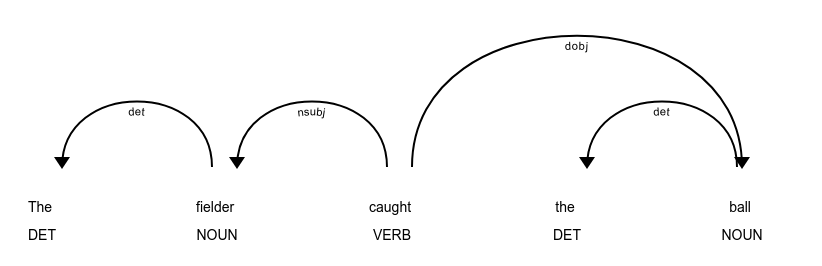
\includegraphics[width=\textwidth]{background/dependency_graph.png}
\label{dependency-graph}
\end{figure}

\subsubsection{Constituency Parsing}

Constituency Parsing is a form of syntactic parsing which assigns a structure to a sentence created by a context-free grammar \cite{RefWorks:RefID:28-jurafsky2014speech}.
This approach aims to group words into constituents, a group of words that behave as a single unit.
For example, one may group a sequence of words surrounding a noun into a noun phrase such as \emph{the Imperial students}.
Words grouped into constituents can be used as an intermediate form for semantic analysis and checking whether a sentence is grammatically correct.
In the context of this project, it will be utilised as a part of atomic sentence extraction.


The resulting structure produced by constituency parsing is a parse tree. 
An example of a tree parsed by a constituency parser can be seen in \ref{constituency-graph}.

\begin{figure}[h]
% https://parser.kitaev.io/
% INSERT https://spacy.io/universe/project/self-attentive-parser
% TODO find where labels are defined.
\caption{Parse tree of \emph{The fielder caught the ball.} as generated by spacy Berkley Neural Parser.}
\centering
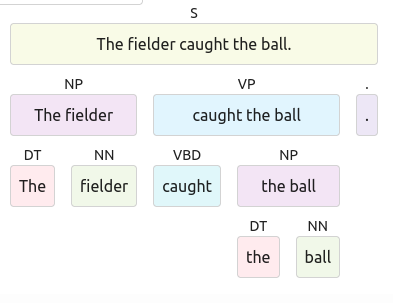
\includegraphics[width=0.8\textwidth]{background/constituency parse.png}
\label{constituency-graph}
\end{figure}

% How is it done if need more content?

% \section{Other Relevant Machine Learning Topics}
% 
% TODO
% 
% \subsection{Video Processing}
% 
% \subsubsection{Convolutional Neural Networks}
% 
% % Check those from their papers.
% 
% % Check more stuff from computer vision.
% 
% \subsubsection{Feature Extractors}
% 
% \subsection{Attention}






\chapter{Related Work}

\section{Inherited Work}
\label{inherited-work}

This thesis has not been started from scratch.

% TODO reference paper %
The project itself is a continuation of the \emph{Automatic Concept Extraction for Concept Bottleneck-based Video Classification} \cite{RefWorks:RefID:16-2021automatic} which my supervisors authored.
This paper is currently under review for the \href{https://iclr.cc/}{ICLR 2022} conference. \\

In this work, the following has been completed:

 Concept Discovery and Extraction Module (CoDEx) is proposed, which automatically uses video explanations to extract concepts.
 
 - Model has been evaluated to validate it obtains competitive performance with standard end-to-end models.
 
 - The concept-based architecture has been augmented with the attention mechanism, which enables verifying how important each concept is for a decision.
 
 - Two public datasets are constructed, MLB-V2E and MSR-V2E. Both combine crowd-sourced explanations with short video sequences. The difference is that the MSR-V2E focuses mainly on general videos while MLB-V2E is baseball-related.
\\

The CoDEx is a vital element of the project.
The presented Concept Discovery and Extraction Module in the paper consists of 6 stages: cleaning, extraction, grouping, completion, pruning, and vectorisation.
The cleaning stage removes videos/explanations which are corrupted.
The extraction step uses a constituency parser and a rule-based approach to determine whether a part of the sentence  should be included as a candidate concept. 
The rules are shown in the following table.

\begin{center}
\begin{tabular}{ |p{2cm}|p{12cm}|  }
 \hline
 \multicolumn{2}{|c|}{Rules determining whether a candidate concept should be included or excluded} \\
 \hline
 rule name & rule \\
 \hline
 Inclusion 1 & noun/pronoun → auxillary (optional) → particle (optional) → verb (optional) \\
 Inclusion 2 & noun/pronoun → auxiliary whose lemma is 'be' → any token \\
 Exclusion & subordinating conjunction \\
 
 \hline
 
\end{tabular}
\label{inclusion-exclusion-rules}
\end{center}

The completion stage looks up for concepts identified in some explanations while not other ones due to the behaviour of the constituency parser.
That stage is done by the substring lookup of existing concepts in all sentences where previous steps did not find that concept.

The grouping step attempts to group concepts with similar meanings using agglomerative clustering \cite{RefWorks:RefID:13-mullner2011modern}. 
It also removes concepts that have a small frequency.

The pruning stage attempts to keep highly informative concepts by picking the smallest concept subset such that the mutual information \cite{RefWorks:RefID:30-mackay2004information} between the label and a concept vector does not fall below a certain percentage $\gamma$.
This problem is not solved precisely, but rather concepts are inserted using a greedy approach until the mutual information between the label and the newly constructed vector is not below a percentage $\gamma$.


The vectorisation constructs the N x K concept matrix, where K is the number of concepts and N is the number of data points. 
The cell (n, k) is one if the concept k occurs for the data point n, zero otherwise.

\section{Video Classification}

Even though the work on video classification is not closely related to this thesis's contributions, it should serve as a performance benchmark of the entire system.

There are a few popular datasets for video classification out there, such as YouTube-8M \cite{RefWorks:RefID:10-abu-el-haija2016youtube-8m:} and Kinetics \cite{RefWorks:RefID:9-carreira2017quo}.
The YouTube-8M \cite{RefWorks:RefID:10-abu-el-haija2016youtube-8m:} is an extensive benchmark for general video classification with around 8 million clips and 4800 visual entities.
Mao et al. \cite{RefWorks:RefID:4-mao2019hierarchical} achieved very high performance on the YouTube-8M dataset using a deep convolutional graph neural network and a multi-level feature extractor.
Kinetics-700 \cite{RefWorks:RefID:14-carreira2019short} dataset is the latest version of the popular Kinetics dataset, which contains 700 human action classes and around 650000 video clips.
The top-performing model at the dataset has been designed by Yan et al. which uses Multiview Transformers for Video Recognition. 
The core idea of this approach is to input multiple different "views" of an input video into a transformer model to achieve better results.
This approach resulted in a model with an accuracy of 82.2\% on the Kinetics-700 dataset with the top-5 accuracy of 95.7\%.

YouTube-8M and Kinetics datasets are somewhat different to the dataset the majority of the project will address.
The MLB-V2E sequences look very similar, given that all of the sequences start with a pitcher throwing a ball.

A dataset much more closely related to our problem is the MLB-YouTube \cite{RefWorks:RefID:3-piergiovanni2018fine-grained} dataset.
The segmented video classification part of this dataset is the base for the MLB-V2E \cite{RefWorks:RefID:16-2021automatic} dataset which also includes crowd-sourced explanations. 
The MLB-YouTube dataset is quite different from the alternatives discussed in this section because the scene is very similar in all videos, only a single camera view is used, and the activity itself is only different because of the movement of one person.
The MLB-YouTube paper validates the InceptionV3 \cite{RefWorks:RefID:49-szegedy2016rethinking} and I3D \cite{RefWorks:RefID:9-carreira2017quo} networks performance on the constructed datasets shown in the table below.
These results should serve as a guide for the results of this project.

\begin{center}
\begin{tabular}{ |p{2cm}|p{1cm} p{1cm} p{1cm} p{1cm} p{1cm} p{1cm} p{1cm} p{1cm}|  }
 \hline
 \multicolumn{9}{|c|}{Per-class average precision for the multi-class baseball classification} \\
 \hline
 Method & Ball & Strike & Swing & Hit & Foul & In Play & Bunt & Hit by Pitch \\
 \hline
 Random & 21.8 & 28.6 & 37.4 & 20.9 & 11.4 & 10.3 & 1.1 & 4.5 \\
 InceptionV3 & 66.9 & 93.9 & 90.3 & 90.9 & 60.7 & 89.7 & 12.4 & 29.2 \\
 I3D & 62.5 & 91.3 & 88.5 & 86.5 & 47.3 & 75.9 & 16.2 & 21.0 \\
 \hline
 
\end{tabular}
\label{inclusion-exclusion-rules}
\end{center}


\section{Definition of Concept in Other Settings}

There are different angles to the definition of concepts in various works.
As mentioned, this project defines a concept as a syntactic generalisation of an atomic sentence.
However, this approach is not common in other works which do concept extraction.


Formal concept analysis \cite{RefWorks:RefID:31-ganter2012formal} is a method for knowledge representation based on the lattice theory which can be used to extract hierarchical concepts.
It defines two fundamental notions: a formal context and a formal concept. 
Formal context K := (G, M, I) consists of a set of objects G, set of attributes M and relation I on (G, M).
If (g, m) $\in$ I, object g has attribute m.
Using these attributes, set A$' $ is defined containing all attributes common to the objects in a set of objects A.
Additionally, set B$' $ contains objects that have all attributes in the set of relations B.
From these definitions, formal concept of context (G, M, I) is defined as a pair (A, B) such that A $\subseteq$ G, B $\subseteq$ M, B$' $ = A and A$' $ = B.

The Formal Concept Analysis with text analysis is mainly used to construct the concept hierarchy, where a concept refers to a phrase containing two words.

For example, work by Cimiano et al. \cite{RefWorks:RefID:32-cimiano2005learning} extracts verb/subject, verb/object/ and verb/prepositional phrase as candidate concepts.
Moreover, the Formal Concept Analysis is used by Anoop et al. \cite{RefWorks:RefID:33-anoop2019extracting} to extract concepts with their relationships from unstructured text.
The authors manually extract stemmed noun phrases as key phrases and use indications such as "is-a" to generate a formal context table.
This table is then used to extract hierarchical concepts.

On the other hand, TaxoLearn \cite{RefWorks:RefID:34-dietz2012taxolearn} by Dietz et al. does not use Formal Concept Analysis but also extracts noun phrases as concepts. The relevance of noun phrases is checked by computing how often they appear in a particular context compared to other contexts. It also uses a hierarchical clustering algorithm to construct a taxonomy.

Moreover, approaches such as the one by Koh et al. \cite{RefWorks:RefID:35-koh2020concept} define concepts as properties that the image may have. These properties need to be provided beforehand.

Finally, work such as the one by Fan et al. \cite{RefWorks:RefID:50-fan2004semantic} use expert defined terms, such as \emph{Lecture Presentation for Gastrointestinal Surgery}, as semantic concepts. 


\section{Concept-Based Explanations for Images and Text}

Concept-based explanations for images and text attempts is a more straightforward related problem.
Koh et al. \cite{RefWorks:RefID:35-koh2020concept} predict a set of pre-labelled concepts which they use to make a final classification.
The pipeline by Koh et al. is similar to the pipeline that will be used in this project, just that the concepts are automatically extracted instead of provided.
Yeh et al. \cite{RefWorks:RefID:36-yeh2019completeness-aware} propose a method that automatically extracts sets of pixels from an image that represent valuable concepts.
Similarly, Ghorbani et al. \cite{RefWorks:RefID:37-ghorbani2019automatic} propose another method that automatically extracts a set of visual concepts which are meaningful to humans.
All outlined methods are based on visual concept extraction, unlike this project's concept extraction, which will mainly focus on the events/actions in the baseball video sequence.


\section{Video Explanation}

Another related problem is that of Video Explanations. This project may even explore it at a later stage within the context of a concept extraction pipeline.

One famous dataset for video understanding is the MSR-VTT dataset \cite{RefWorks:RefID:40-jun2016msr-vtt:}. It is a large scale dataset with more than 10000 video clips in 257 popular categories of a video search engine.
Each video is annotated with roughly 20 sentences. 
A few different approaches for tackling this issue are presented as viable options in the paper, such as 2D Convolutions, 3D Convolutions, and RNNs.
One of the most performant methods on this dataset is CLIP2TV \cite{RefWorks:RefID:41-gao2021clip2tv:}, which utilises transformer-based techniques for both video and text representation.


The authors of the MLB-V2E \cite{RefWorks:RefID:16-2021automatic} have also constructed the MSR-V2E \cite{RefWorks:RefID:16-2021automatic} dataset, which uses the clips made available by the MSR-VTT and provides new classification labels and explanations.
This dataset will likely be used for the evaluation of this project.

\section{Semantic Concept Video Classification}

Semantic Concept Video Classification attempts to predict a set of predefined concepts from a video.
Predicting a set of predefined concepts from a video is closely related to a part of the pipeline in this project, which indicates which extracted concepts occur before predicting the outcome. 

The work by Fan et al. \cite{RefWorks:RefID:50-fan2004semantic} tries to predict semantically defined concepts by medical experts.
The paper proposes using salient objects, which are visually-distinguishable video components that human semantics understands, to model these semantical concepts.
Examples of notions salient objects attempt to represent are a face, voice, or a lecture slide.
Despite its benefits, the semantics of salient objects is quite simple, and it does not model relationships that happen over multiple frames in a video.
Newer work by Fan et al. \cite{RefWorks:RefID:51-jianping2007incorporating} also incorporates the possibility of a hierarchical concept classification. The approach also predicts atomic video concepts before constructing the higher-level ones and existing concept ontology.

Assari et al. \cite{RefWorks:RefID:52-assari2014video} represent a video by the co-occurrence of the semantic concepts before applying a classifier.
The concepts in this work are also predefined, but they represent a set of events rather than a set of objects.




% Possible background additions:
% Positive/Negative examples ILASP.
% Semantic parsing maybe.

% Add a box plot somewhere


% TODO: Alessandra feedback: use running examples because it's easier to understand that way
% TODO: Alessandra feedback: do comparison with semantic entailment if it is
\chapter{Solving NLP Tasks Logically}
\label{solving-nlp-tasks-logically}


Logical representations have an important place in the Natural Language Processing field.
Semantic parsing \cite{RefWorks:RefID:28-jurafsky2014speech} is a famous task that aims to convert a natural language input that captures the meaning of that input.
After all, having a sentence in a logical form allows reasoning about it to form new conclusions.

However, in this chapter, the logic is used in a slightly unconventional manner for NLP.
It is an intermediate representation for a sequence-to-sequence problem where it captures only the syntax of the text rather than its meaning.
The current state of the art approach for sequence-to-sequence problems, such as language translation, uses transformers. 
Nevertheless, seq2seq transformers would perform poorly with available datasets for the two problems tackled in this chapter.
The datasets consisting of ~100 examples are too small for a model with billions of parameters to be able to generalise.
% INSERT Imdb dataset reference 
Transformer fine-tuning is usually done on tens of thousands of examples, such as the IMDB Movie Reviews dataset. \\
% INSERT reference second year notes.
On the other hand, logic-based learning systems can generalise well from a tiny number of examples, making them suitable for the problems presented in this chapter. \\


In this chapter, the following topics are presented:
\begin{itemize}
    \item Introduction of atomisation and generalisation tasks
    \item A logical approach to solving the generalisation task.
    \item A logical approach to solving the atomisation task.
    \item Implementation details for solving these two problems.
    \item Evaluation of the two methods.
\end{itemize}



% TODO: Alessandra feedback: add more introduction, namely the drawing in alessandra-feedback-diagram - one box is for the atomiser (symbolic atomisation transformer), another one for generalisation - they work on sentences to sentences
% TODO: Alessandra feedback: go into how both atomisation and generalisation works briefly
% TODO: Alessandra feedback: add more introduction, namely the drawing in alessandra-feedback-diagram

% From what I understood Ale's feedback is decided on the Nuri's paper - if there is time look into his papers for inspiration
 
\section{Sequence2Sequence Tasks}

The two tasks that have been tackled using logic based learning approach are \textbf{sentence} \textbf{atomisation} and \textbf{generalisation}.

The former converts a declarative sentence into one or more \textbf{atomic sentences}, while the latter converts an \textbf{atomic sentence} into one or more \textbf{concept sentences}.

% TODO: Alessandra feedback: no need for a subsection. Merge with the previous one
\subsection{Sentence Type Definitions}
\label{sentence-type-definitions}

\textbf{Atomic Sentence:} A sentence that cannot be decomposed into multiple valid sentences. \\
% TODO add reference %
Note that this is equivalent to the definition used in logic.
However, the sentence structure considered in this project is often much more complex than the one considered in logic.\\
% INSERT insert simple predicates definition reference %
An \textbf{atomic sentence} should only contain simple predicates, eliminating compound and complete predicates from a sentence.


\textbf{Concept Sentence:} A syntactic generalisation of an atomic sentence, which satisfies the following three conditions:
\begin{enumerate}
% TODO: Alessandra feedback: valid -> syntactically well-formed -> give examples for what it means for a sentence to be syntactically well-formed
    \item It is a valid sentence in its own right.
    \item True if the atomic sentence is.
    \item Obtained only through syntactic manipulation of an atomic sentence, a result of modifying the syntax tree of the sentence.
\end{enumerate}

% TODO: Alessandra feedback: argue that concept sentence is any syntactically well formed substring of an atomic sentence.
Concept sentences are sometimes referred to as \textbf{(syntactic) generalisations} of a sentence in this report.


\begin{example}
Splitting a given sentence into all its concepts sentences.

Starting from the sentence:  
\begin{verbatim}
The batter caught the ball in the air and sent it into the left field.
\end{verbatim}
we can extract the following atomic sentences: 
\begin{verbatim}
The batter made contact with the ball in the air. 
The batter sent it into the left field.
\end{verbatim}
From these two sentences, we can obtain four concept sentences: 
\begin{verbatim}
The batter made contact with the ball in the air.
The batter made contact with the ball.
The batter sent it into the left field.
The batter sent it into the field.
The batter sent it.
\end{verbatim}

\end{example}

% TODO: Alessandra feedback: no need for a subsection. Merge with the previous one
\subsection{Purpose of the Tasks}

The two tasks mentioned are a part of the Concept Bottleneck pipeline discussed in greater detail in Chapter \ref{concept-bottleneck-pipeline}
These two tasks are used in sequence as a replacement for the extraction part of the original CoDEx (Concept Discovery and Extraction) pipeline \ref{inherited-work}.

The reason the project aims to extract all concept sentences from a particular sentence is two-fold:
\begin{enumerate}
    \item Concept sentences help associate differently worded explanations of the same concept.
    \item The final generated sentences are immediately usable for explanations.
\end{enumerate}

% TODO: Alessandra feedback: add part 2 of the diagram from the introduction but now show the syntactic parse trees to showcase what we are doing in this part
% TODO: Alessandra feedback: talk about the definition of the learning task associated with the background.
% TODO: Alessandra feedback: make background/language_bias \paragraph or something similar so that they don't appear in the table of contents
\section{Solving Concept Generalisation}
\label{solving-generalisation-task}

\subsection{Logical Encoding}
\label{logical-encoding}

In this subsection, we showcase how the example sentences are encoded logically and the pipeline used at test time to generate solutions.
All encodings are compatible with the Answer Set Programming \cite{RefWorks:RefID:1-lifschitz2008answer} paradigm.
The solution learning is described in the following subsection (\ref{encoding-the-learning-task}), which relies on the encodings presented in this subsection. 


A solution to the \textbf{concept generalisation} task is learned using the Inductive Logic Programming tool ILASP \cite{RefWorks:RefID:18-law2020ilasp}.

\subsubsection{Encoding the Example Premise}

% TODO: delete this because it is discussesed in the implementation
\textbf{Generalisation} examples consist of a given sentence followed by one to many sentences, which are ways in which the provided sentence can be generalised/atomised.
For instance, here is a possible \textbf{generalisation} example:
\begin{verbatim}
"It was a fast ball.", "It was a ball. It was a fast ball."
\end{verbatim}


We first need to define a way to convert the sentences into a logical representation that we could use to reason about the sentence structure.
Ideally, a sentence representation should satisfy the following criteria:
\begin{itemize}
    \item Word dependency capture --- The representation should capture dependencies between words to determine whether a word is crucial to the meaning of a sentence.
    \item Similar meaning $\rightarrow$ similar encoding --- Slight word variations such as words replaced by synonyms should be encoded similarly. The task becomes easier for the learner when the words with the same meaning are captured by the exact representation.
    \item Compactness --- Smaller representations are quicker to process. 
    \item Domain independence --- We want to apply the generalisation task in various domains, so the representation should not contain domain-specific information.
    \item Interpretability --- It should be clear what the representation encodes. We can translate the learned ILASP solution into English if the predicates are interpretable. Hence, we can verify whether the system learned spurious correlations or valuable rules.
    \item Reconstuctability --- One should be able to reconstruct a sentence as the final output of the task needs to be a correct sentence.
\end{itemize}


% INSERT word2vec reference
A common approach to encoding a sentence involves using dense-vector contextualised embeddings of words, such as the ones produced by Word2vec.
Dense-vector embeddings are practical because they are compact and tend to capture the semantics of words (i.e. map similar words to similar value embeddings).
Transformers improve upon these embeddings by using the self-attention mechanism to provide an even better representation of a sentence.

However, dense-vector embeddings are not interpretable, making them difficult to use with our problem. 
The learning approach that we have used follows a similar idea of trying to capture semantic relationships within a sentence.
We utilise the \textbf{dependency parse tree} as a basis for the \textbf{generalisation} task as it captures syntactic relationships between words.
% INSERT reference NLP notes
Note that the syntactic relationships captured approximate the semantic relationships between words.
In addition, words themselves are put into logical predicates, making the sentences reconstructible.

The dependency tree gives rise to the following predicates:
\begin{verbatim}
    dep(l, token1, token2).
    root(token).
    token(token, string).
\end{verbatim}

It represents that there exists an arc from \verb_token1_ to \verb_token2_ with label \verb+l+ which are converted back to string form with \verb_token_ predicate.
In addition, \verb_root_ encodes which token is the root of the sentence.

\begin{example}
\label{logical-encoding-example}
Encoding \textit{he threw a fast ball}, with a dependency graph shown in \ref{example-dependency-graph}:
\begin{enumerate}
    \item Convert each token in the tree to a logical form
    \begin{verbatim}
        token(tok0, "he").
        token(tok1, "threw").
        token(tok2, "a").
        token(tok3, "fast").
        token(tok4, "ball").
    \end{verbatim}
    \item Convert arcs and roots of the tree to predicates:
    \begin{verbatim}
        root(tok1).
        dep(nsubj, tok1, tok0).
        dep(dobj, tok1, tok4).
        dep(det, tok4, tok2).
        dep(amod, tok4, tok3).
    \end{verbatim}
\end{enumerate}
\end{example} 

\begin{figure}[h]
\caption{Dependency graph of \emph{He threw a fast ball.}}
\centering
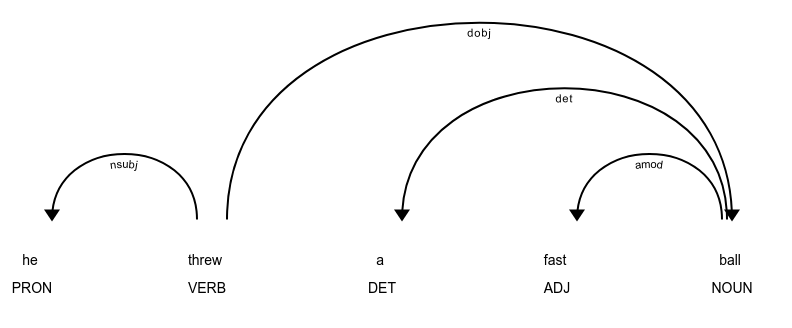
\includegraphics[width=\textwidth]{solving-nlp-tasks-logically/example_dependency_tree.png}
\label{example-dependency-graph}
\end{figure}

Reflecting on the criteria outlined at the start of the section, we can see that it is mainly satisfied by the encoding. 
Even the similar meaning $\rightarrow$ similar encoding is captured somewhat in the context of this problem.
The two sentences which only differ by one synonym would be identically represented by the \verb_dep_ predicates, resulting in any model treating them similarly.
For example, the sentences:
\begin{verbatim}
    The batter hit the ball. The hitter hit the ball.
\end{verbatim}
would have the equal \verb_dep_ predicate representation. 
However, the sentences:
\begin{verbatim}
    The batter hit the ball. The ball was hit by the batter.
\end{verbatim}
would not have similar representations.
This representation drawback did not end up being a hurdle for the current dataset.

\subsubsection{Encoding the Example Target}
\label{encoding-the-example-target}


After the example observation, it became clear that concept sentences contained only the words used in the premise.
We could model the problem in this section as to whether or not we want to include the word in a concept sentence.
That goal is denoted with a predicate:
\begin{verbatim}
   in_generalised_sent(t).
\end{verbatim}
which represents that a token \verb+t+ is included in the concept sentence.
The possibility of multiple concept sentences existing is modelled using multiple answer sets.
\begin{example}
\label{example-encoding-target}
Encoding \textit{he threw a ball} as a generalisation of \textit{he threw a fast ball}:

From the previous example (\ref{logical-encoding-example}), we have:
\begin{verbatim}
    token(tok0, "he"). token(tok1, "threw"). token(tok2, "a"). 
    token(tok3, "fast"). token(tok4, "ball").
\end{verbatim}
So, we the example target is encoded as:
\begin{verbatim}
    in_generalised_sent(tok0). in_generalised_sent(tok1). 
    in_generalised_sent(tok2). in_generalised_sent(tok3). 
\end{verbatim}

\end{example}

\subsection{Encoding the Learning Task}
\label{encoding-the-learning-task}

Learning a solution with ILP is different from determining a solution with Deep Learning.
% INSERT reference to KR notes
Inductive Logic Programming uses a different level of knowledge representation commitment than Deep Learning.
Deep Learning approaches do not give any inductive bias to a machine. 
The model must learn how to solve the problem from the data only. \\
On the other hand, Inductive Logic Programming requires more human-generated knowledge representation.
In particular, the logical structure is encoded to the learner, which is encouraged to find all possible theories within that structure and return the best one. 
Because of this property, the Inductive Logic Programming paradigm can incorporate existing knowledge into the final solution, making the task easier to solve.

The following subsection demonstrates how the \textbf{generalisation} task has been solved with ILASP \cite{RefWorks:RefID:18-law2020ilasp}, a state-of-the-art ILP system.

% TODO: Alessandra feedback: describe a problem with learner first before going into a hand-crafted solution (after learning)
% Argue that a hand-crafted solution should be something a human engineered ground truth model

\subsubsection{Background Knowledge Construction}

Here is the background knowledge used for the \textbf{generalisation} task.
\begin{verbatim}
token(T) :- root(T).
token(T) :- dep(_, T, _).
token(T) :- dep(_, _, T).
label(L) :- dep(L, _, _).

% there must be a token in any concept sentence
:- #count{T : in_generalised_sent(T)}0.
\end{verbatim}
The first four rules define unary predicates used as types in language bias, while the final rule encodes that a generalised sentence should not be empty.

\subsubsection{Language Bias}

The construction of the language bias was done by first designing a hand-crafted ASP solution that tackles the task well, followed by encoding all predicates used in that solution to ILASP.
The hand-crafted solution helps find the structure logical structure the learner should know.
ILASP should then be able to find a better solution within those constraints.


% TODO: Alessandra feedback: Justify a 0 1 boundary
The problem is modelled as a choice of whether a particular token (word) should always be included or sometimes be included in the solution, which the following types of rules can represent.
\begin{verbatim}
in_generalised_sent(T) :- ...
0 {in_generalised_sent(T) } 1 :- ...
\end{verbatim}

This gives rise to the following language bias:
\begin{verbatim}
#modeh(in_generalised_sent(var(token))).
#modeha(in_generalised_sent(var(token))).

#modeb(in_generalised_sent(var(token))).
#modeb(root(var(token))).
#modeb(dep(const(label), var(token), var(token)), (positive)).

#bias("
% Only allow rules 0 { in_generalised_sent(V1) } 1.
% Eliminates all generated rules that where lhs of 
% the curly brace is >= 1.
:- in_head(_), lb(1).
").

% Disallow 2+ in_generalised_sent predicates occurring within {}.
#disallow_multiple_head_variables.

\end{verbatim}

% TODO: Alessandra feedback: what would happen if we only had #pos examples.
% TODO: Alessandra feedback: Argue that the size is because of the number of constants that we have. 
\subsubsection{Example Encoding}
\label{example-encoding}

As mentioned, \textbf{generalisation} examples consist of a given sentence followed by 1 to many concept sentences.
We need to convert those representations into ILASP examples.
% INSERT: refer to background where a more formal definition is provided %
ILASP allows defining two types of examples as outlined more formally in \ref{examples-in-ilasp}.
\begin{itemize}
    \item positive (\verb_#pos_) - an example which should be by at least one answer set.
    \item negative (\verb_#neg_) - an example that any answer set should not extend.
\end{itemize}

Ideally, we want the solution learned by ILASP to produce the number of answer sets equal to the number of generalisations.
Using these two constructs, we can define that we want exactly one answer set for each possible generalisation. \\
It is done by creating a positive example for each sentence we wish to produce. 
In addition, a negative example is produced with the \verb_goal_ predicate in the exclusion for each text sentence example.
The \verb_goal_ predicate, defined only in the contexts of negative examples, is true if \verb+in_generalised_sent+ atoms correspond precisely to a positive example.


\begin{example}
Generating ILASP-compatible generalisation examples for \textit{"He threw a fast ball.", "He threw a ball. He threw a fast ball."}

% INSERT reference to previous section %
1. Convert the premise sentence to logical form, as shown in example \ref{logical-encoding-example}.

2. For each possible generalisation, create a positive example. The context consists of predicates produced in step 1, while the inclusion/exclusion of appropriate \verb+in_generalised_sent+ tokens (example \ref{example-encoding-target}). The concept sentence \textit{He threw a ball.} yields the following example:
\begin{verbatim}
#pos(example_id@noise_penalty,
{in_generalised_sent(tok0), in_generalised_sent(tok1), 
 in_generalised_sent(tok2), in_generalised_sent(tok4), 
 in_generalised_sent(tok5)},
{in_generalised_sent(tok3)}, % tok3 = "fast"
{
% all the predicates generated in step 1
}).
\end{verbatim}

3. The negative example is generated as follows:
\begin{verbatim}
#neg(example_id@noise_penalty,
{ },
{ goal },
{
% all the predicates generated in 1)

% He threw a fast ball.
goal :- in_generalised_sent(tok0), in_generalised_sent(tok1), 
        in_generalised_sent(tok2), in_generalised_sent(tok3), 
        in_generalised_sent(tok4), in_generalised_sent(tok5).
% He threw a ball.
goal :- in_generalised_sent(tok0), in_generalised_sent(tok1), 
        in_generalised_sent(tok2), in_generalised_sent(tok4), 
        in_generalised_sent(tok5)}, not in_generalised_sent(tok3).
}).
\end{verbatim}
\end{example}

All of the examples constructed have a \verb+noise_penalty=1+ as the \textbf{concept generalisation} examples may be noisy.


% TODO: Alessandra feedback: scaling up should be a separate section
\subsection{Managing Learning Scalability Constraints}

% INSERT reference for this. %
A considerable challenge with logic based learning systems, such as ILASP, is a lack of scalability when dealing with large scale AI problems compared to other forms of machine learning. \\
For the \textbf{generalisation} task, two challenges needed to be mitigated: 
\begin{itemize}
    \item Lack of scalability w.r.t size of the hypothesis space -- This issue arises due to ILASP enumerating search space $S_M$ in full before finding a solution.
    \item Extreme RAM consumption during task solving.
\end{itemize}

\subsubsection{Reducing the hypothesis space size}
\label{reducing-the-hypothesis-space-size}

For example, consider the following simplified language bias definition:
\begin{verbatim}
#modeh(in_generalised_sent(var(token))).
#modeb(in_generalised_sent(var(token))).
#modeb(root(var(token))).
#modeb(dep(const(label), var(token), var(token))).

... all the constant definitions ...
\end{verbatim}

% INSERT Might be benficial to include a table how each rule reduced the search space size.

It took over 13 hours to generate an entire search space on a machine with an Intel Core i7 10510U 1.80GHz / 4.90GHz processor and 16 GiB of RAM.

FastLAS \cite{RefWorks:RefID:19-law2020fastlas:} is a system designed to alleviate this particular constraint, but it can only deal with a restricted version of the learning task.
Its inability to produce a solution with multiple answer set made it inapplicable for the current problem.

% INSERT reference to Mark's website
The scalability issue was instead tackled using meta-level definitions of the hypothesis space, which allow much greater flexibility than simple \textit{modeb}, \textit{modeh} statements. 
They allow constraining how rules are generated using ASP syntax, removing rules that we do not want as a part of the learned solution.
We always want to remove the rules whose body could never be satisfied.

Here are some examples of they are utilised to restrict the search space presented in this section:
\begin{verbatim}
% Idea #1: Dep represents an arc in a tree. This allows 
% cutting out rules which are impossible to be satisfied.
    
% It is impossible to have more than 1 root per example.
:- #count{T : body(root(T))} > 1.

% Trees cannot have a relation to itself.
:- body(dep(_, X, X)).
:- body(naf(dep(_, X, X))).

% A tree is not symmetric.
:- body(dep(_, X, Y)), body(dep(_, Y, X)).

% No dependency can go to the root
:- body(root(X)), body(dep(_, _, X)).

% Idea #2: Only allow two dep rules to occur in a body
% under certain conditions. 

% Pairs of dependency tags which can co-occur.
% Much smaller set of all possible pairs.
dep_chain(prep, pobj).
dep_chain(pobj, amod).
...

% Allow any rule with at most one dep predicate
allowed_dep_rule :- #count{L, V4, V5 : body(dep(L, V4, V5))} <= 1.
% Allow rule with two dep predicates if it is labels are white-listed
% by dep_chains and tokens are chained too.
allowed_dep_rule :- body(dep(L1, _, V2)), body(dep(L2, V2, _)), 
                    dep_chain(L1, L2), 
                    #count{L, V4, V5 : body(dep(L, V4, V5))} = 2.

:- not allowed_dep_rule.

% Idea 3: Remove rules that where simpler rules would suffice.

% Rule with root(V3) where V3 is not used in any dep is not needed.
% This predicate is trivially satisfied since every sentence has a 
% root.
:- body(root(X)), not body(dep(_, X, _)), not body(dep(_, _, X)), 
   body(dep(_, _, _)).

% If we have a in_generalised_sent predicate there must be some logic 
% related to it.
% This predicate is trivially satisfied otherwise, since the 
% background requires that at least one must always exist.
:- body(in_generalised_sent(X)), not body(dep(_, X, _)), 
   not body(dep(_, _, X)).


\end{verbatim}

These modifications allowed the search space generation times to take less than a minute, starting from over 13 hours.
The final search space consisted of only 3652 rules.


% TODO: Alessandra feedback: avoid using OOM acrynoym - replace with out-of-memory/lack of memory
\subsubsection{Avoiding OOM Errors}
\label{avoiding-oom-errors}

ILASP memory consumption is drastic even for the simpler of the two tasks solved logically.
% INSERT memory graph drawn on batch machine over time for generalisation.
The memory consumption graph over time is outlined in \ref{generalisation-memory-graph}.
As seen in the plot, the graph is at around 15 GB of RAM at about 15-hour mark.
So, to prevent the usual 16 GB machines from going out of memory, the execution is terminated after 15 hours, and the best solution found until that point is returned.
This technique prevents the ILASP process from exceeding the memory limit while returning a high-quality result.

% INSERT reference to PyLASP doc
The aforementioned ILASP behaviour modification is possible through the use of PyLASP scripts.

\begin{figure}[h]
\caption{Comparison of the ILASP solution performance and memory consumption over time. A lower ILASP score corresponds to a better solution.}
\centering
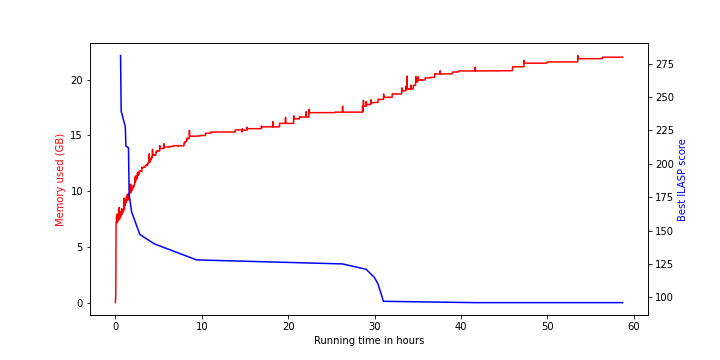
\includegraphics[width=\textwidth]{solving-nlp-tasks-logically/generalisation_memory_vs_best_score.png}
\label{generalisation-memory-graph}
\end{figure}

\subsection{Final Solution}

The final solution is obtained by running ILASP with background, language\_bias, examples and the custom PyLASP script.
In addition, all ILASP tasks were run with the \verb+--restarts+ flag, which can help reduce the running time of a program.

% INSERT reference to evaluation part of this section
The results of the performance of the \textbf{generalisation} task can be found in \ref{concept-generalisation-results}.


% TODO: Alessandra feedback: argue that atomistaion is a 3-step process - generate logical form + apply rules + reconstruct the data
% TODO: Alessandra feedback: add diagram with dependency trees - alessandra feedback-diagrams.png has a sketch

% TODO: Alessandra feedback: add part 1 of the diagram from the introduction but now show the syntactic parse trees to showcase what we are doing in this part
% TODO: Alessandra feedback: argue why the atomisation task is harder than the generalisation
\section{Solving Atomisation Task}
\label{solving-atomisation-task}

The solution to the atomisation task has only been hand-crafted rather than learned.
This section will highlight the idea behind the hand-crafted solution and demonstrate that ILASP is currently not scalable enough to learn a solution that is at least as good as the hand-crafted one.

\subsection{Shared Encoding Logic with Generalisation}

Due to the domain similarity of the two tasks, almost the entire Logical Encoding subsection (\ref{logical-encoding}) is fully applicable for the \textbf{atomisation} task with the following caveat:
\begin{itemize}
    % INSERT reference
    \item Encoding the Learning Target (\ref{encoding-the-example-target}) --- The goal for the \textbf{atomisation} task is denoted with \verb+in_atomised_sent+.
\end{itemize}

% TODO: Alessandra feedback: summarise the rules in English first before encoding them symbolically
% TODO: Alessandra feedback: include a table with two columns (predicate name, description) before which highlight what each of the predicates mean (so candidate_start is ...)
\subsection{Hand-crafting the Atomisation Solution}
\label{hand-crafting-the-atomisation-solution}

Consider the following two sentences and the desired atomisation, as well as the dependency graphs of the premises (\ref{atomisation-examples}):
\begin{lstlisting}
the batter swung and the ball landed 
  $\rightarrow$ the batter swung. the ball landed.
the batter swung and missed 
  $\rightarrow$ the batter swung. the batter missed.
\end{lstlisting}

% TODO Alessandra feedback: argued that there can only be one root in a dependency parse tree.

\begin{figure}[h]
\caption{Dependency graph of two sentences which need to be atomised}
\centering

\includegraphics[width=\textwidth]{solving-nlp-tasks-logically/dependency-graph-one-subj.png}

\includegraphics[width=\textwidth]{solving-nlp-tasks-logically/dependency-graph-two-subj.png}
\label{atomisation-examples}
\end{figure}

The graph illustrates that the terms on both ends of the \verb_conj_ tag should appear in separate sentences. 
Determining splitting tags, tags whose words should be in distinct subsets, is the core idea of the hand-crafted solution.
The words at the edges of these tags become starting points for generating sentences, which are constructed by adding tokens related to current \verb+in_atomic_sent+ tokens.

Following such an approach, the following set of rules was constructed:
\begin{lstlisting}

% Capture tokens at the end of a splitting tag
candidate_start(T) :- splitting_tag(C), dep(C, T, _).
candidate_start(T) :- splitting_tag(C), dep(C, _, T).

% Start splitting tags. Splitting tags must be a part of 
% distinct atomic sentences.
1 { in_atomic_sent(T) : candidate_start(T) } 1.

% Root should be a starting point if there are no 
% splitting tags.
in_atomic_sent(T) :- root(T), not candidate_start(_).

% Tags linking tokens that should be in distinct answer 
% sets, each with an example which sparked the choice:

% The batter swung therefore it is a strike.
% $\rightarrow$ The batter swung. It is a strike.
splitting_tag(ccomp).
% The batter did not swing so it was a ball.  
% $\rightarrow$ The batter did not swung. It is a ball.
splitting_tag(advcl).
% The batter swung the bat but missed the ball.
% $\rightarrow$ The batter swung the bat. The batter missed the ball.
splitting_tag(conj).
% The batter hit the ball in play where it was caught 
% mid air by a defender.
% $\rightarrow$ The batter hit the ball in play. It was caught mid air by a defender.
splitting_tag(relcl).



% Include all incoming relationships except candidate_starts. 
% This allows us to reach the predicate of the current atomic sentence.
% Atulve's ball was fast and good.
in_atomic_sent(T) :- dep(_, T, T2), in_atomic_sent(T2), not candidate_start(T).


% Incoming relationships first conjunct (conj) should also be included for the second one.
% This holds for conj only. The clauses tend to be self-sufficient.
% Atulve's ball was good and quick. $\rightarrow$ Atulve's ball was quick. Atulve ball was good.
in_atomic_sent(T) :- dep(_, T, T2), dep(conj, T2, T3), in_atomic_sent(T3), not candidate_start(T).


% Include all children tags apart from those that are blacklisted (we do not want and, therefore...)
% Additionally, we do not want to include a candidate_start token. 

% (Therefore) it is a strike
do_not_include(advmod).
% The batter hit the ball (and) it landed far away.
do_not_include(cc).
% Not including punctuation, it should not be in atomic sentences 
do_not_include(punct).
% The umpire ruled (that) the batter did not swing.
do_not_include(mark).
% Skip all the splitting tags
do_not_include(C) :- splitting_tag(C).
in_atomic_sent(T) :- dep(C, T2, T), in_atomic_sent(T2), not do_not_include(C), not candidate_start(T).

 

% Every atomic sentence should have a subject.
% Include the subject of the first conjunct as a part of the second sentence if it does not contain its own.
% The batter swung but missed the ball $rightarrow$ The batter swung. The batter missed the ball.
in_atomic_sent(T) :- dep(nsubj, T1, T), dep(C, T1, T2), splitting_tag(C), in_atomic_sent(T2), not adjacent_subj.

% There is no subject next to any currently included token
adjacent_subj :- dep(nsubj, T1, T2), in_atomic_sent(T1).
adjacent_subj :- dep(nsubjpass, T1, T2), in_atomic_sent(T1).
adjacent_subj :- dep(csubj, T1, T2), in_atomic_sent(T1).
adjacent_subj :- dep(csubjpass, T1, T2), in_atomic_sent(T1).
\end{lstlisting}

\subsection{Atomisation Learning Challenges}

We aimed to learn two things with ILASP for the atomisation learning task:
\begin{enumerate}
    \item A set of rules which extend the number of tokens in the current atomic sentence.
    \item A set of splitting tags.
\end{enumerate}

Constructing the language bias by observing the hand-crafted solution gives results in the following code:
\begin{verbatim}
#modeh(in_atomic_sent(var(token))).
#modeh(splitting_tag(const(label))).

#modeb(1, dep(const(label), var(token), var(token)), (positive)).
#modeb(1, dep(var(label), var(token), var(token)), (positive)).
#modeb(1, splitting_tag(var(label))).
#modeb(1, in_atomic_sent(var(token)), (positive)).
#modeb(1, do_not_include(var(label))).
#modeb(1, candidate_start(var(token))). 
#modeb(1, adjacent_subj).

% Add only negative atoms
#bias("
:- body(adjacent_subj).
:- body(candidate_start(_)).
:- body(do_not_include(_)).
").
\end{verbatim}

The language bias additionally included a more aggressive alternative to the search space reduction method presented in \ref{reducing-the-hypothesis-space-size}, but nevertheless included all of the rules the hand-crafted solution uses. \\
In addition, the examples were constructed in the same manner as in \ref{example-encoding}.
The learning was done on a specialised machine with 500 GiB of RAM, but it still required that an approximate solution be returned after some time (\ref{avoiding-oom-errors}).

% TODO: Alessandra feedback: replace prior with size in the graph legend
% TODO: Alessandra feedback: suggest that ... is the lower bound to solve the task. In addition suggest that if that lower bound was achieved the performance would be at least as good as the ... blue line
% TODO: Alessandra feedback: suggest that the green line is the maximum size the ILASP hypothesis can have
% TODO: Alessandra feedback: talk about ILASP score in background, reference in graph

\begin{figure}[h]
\caption{Comparison of the ILASP atomisation solution performance and memory consumption over time. The maximum prior penalty quantifies the maximum number of predicates ILASP can use in a solution. On the other hand, the example penalty outlines how many examples are not covered by the current solution. The dashed lines represent the values the hand-crafted solution would achieve had it been learned by ILASP.}
\centering
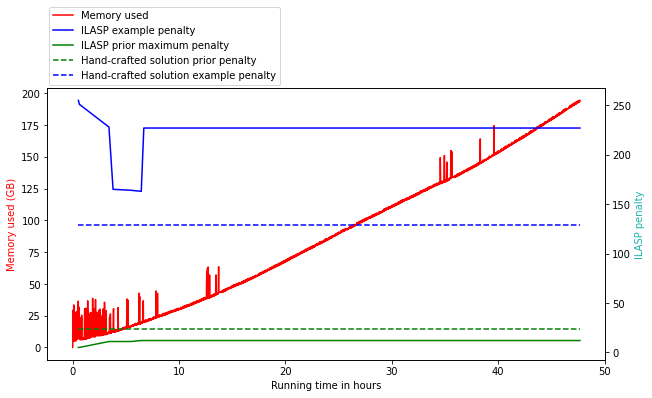
\includegraphics[width=\textwidth]{solving-nlp-tasks-logically/atomisation_memory_vs_best_score.png}
\label{atomisation-memory-graph}
\end{figure}

% INSERT reference Mark theiss% 
ILASP can theoretically find the optimal solution for any noisy task, and the search space represents the hand-crafted solution in full. 
So, we expect the complete run of the task to produce at least as good of a solution as the hand-crafted one.
However, this expectation does not hold within the memory and time constraints available for the \textbf{atomisation} task as shown in \ref{atomisation-memory-graph}.

Observing the maximum prior penalty, we can see that the learner is stuck attempting simple solutions for the duration of the task run. 
The hand-crafted solution uses 24 predicates, whereas the learner never attempted a solution with more than 14 predicates.
This behaviour is quite unlike the one observed for the \textbf{generalisation} task and may even suggest a presence of a bug.

\section{Implementation}

This section presents the implementation design for the learning task and the dependencies used in this code.

\subsection{Atomisation/generalisation procedure}

% TODO: Alessandra feedback: Cut-up this diagram in two one for learning time and one for inference time. With this approach we can replace it to the appropriate report sections.
% TODO: Alessandra feedback: Use ASP Encoder instead of ASP Generator
% TODO: Alessandra feedback: Use Answer Set (Generalised Concept) instead of just Answer Set


\begin{figure}[h]
\caption{Simplified architecture for the concept generalisation part of the CoDEx pipeline.} 
\centering
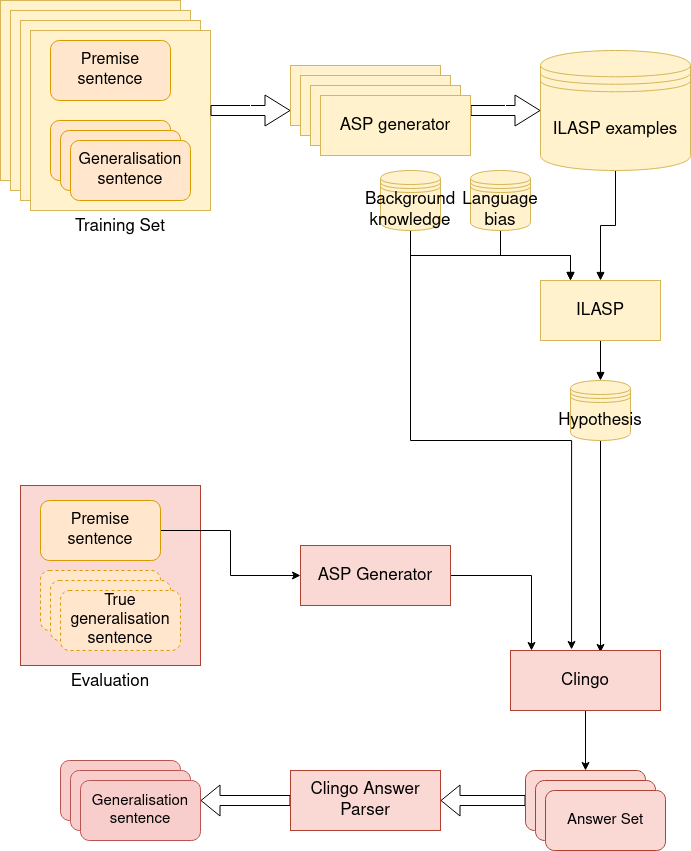
\includegraphics[width=\textwidth]{solving-nlp-tasks-logically/simplified architecture diagram.png}
\label{generalisation-architecture-diagram}
\end{figure}


The architecture diagram of the \textbf{concept generalisation} is shown in \ref{generalisation-architecture-diagram}.
It can be divided into \textbf{learning} and the \textbf{application/evaluation} stage.
The atomisation task uses an almost identical architecture as the \textbf{application/evaluation} stage, where the learned solution is replaced with a hand-crafted one. 
The goal of the \textbf{learning} stage is to learn the hypothesis $H$, which will be able to generalise/atomise any sentence correctly.
Each training example for the learning stage consists of the premise and generalisation sentences provided in CSV format.
The raw examples are written in the following way:

% TODO: Alessandra feedback: This would need to go to either generalisation or atomisation to get the idea of what the data is like.

\begin{center}
\setlength\parskip{0pt}
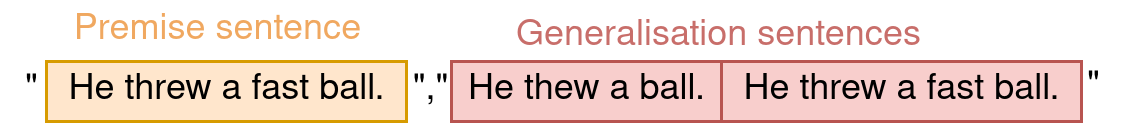
\includegraphics[width=.8\linewidth]{solving-nlp-tasks-logically/raw-generalisation-example.png}
\end{center}

% INSERT spacy/AlunNLP reference
The \textit{ASPGenerator} uses an NLP library to obtain the dependency graph of each sentence, used in the logical representation of an example.

The example files (\textit{ILASP examples} in \ref{generalisation-architecture-diagram}) are persisted since ILASP can only be run as a command line tool.
In addition, the ILASP examples can be split into multiple text files, commonly ten. 
% INSERT condor reference
The split of the files is used to run 10-fold cross validation experiments, parallelised using Condor, a batch processing system.
% TODO: verify this - can be resolved immediately.
The final learned solution (hypothesis $H$), as is the standard practice when doing cross validation, has been produced by training the model with all examples.

% TODO: fix ASP Generator in image
The \textbf{application/evaluation} uses the learned hypothesis in order to split the unknown sentences.
In particular, the process consists of the following stages, visible in \ref{generalisation-architecture-diagram}:
\begin{enumerate}
    \item Conversion to the logical form --- The sentences are converted to the logical form in a manner equivalent to learning encoding. The same module carries out both operations.
    
    % INSERT reference clingo
    \item Answer set solving --- A sentence in the logical form, learned hypothesis and background knowledge are passed to the Clingo answer set solver. Clingo will output all the answer sets of the provided program.
    
    \item Answer parsing --- Each answer set returned corresponds to one generalisation/atomisation sentence. For each \verb+in_generalised_sent+/\verb+in_atomic_sent+ token in an answer set, the actual word corresponding to that token is found. Words are joined in the same order as they appeared in the original sentence. Finally, post-processing techniques (\ref{post-processing-techniques}) are applied to the resulting string to fix possible grammatical issues. 
\end{enumerate}

\begin{example}
Generating all of the generalisations of the sentence \emph{He threw a fast ball.} at test time.

1. Remove . and lowercase all the words in the sentence as a part of pre-processing. The string \emph{he threw a fast ball} is the result of the operations.

2. Convert the sentence to the logical form as shown by the \textbf{example \ref{logical-encoding-example}}.

% INSERT clingo reference
% INSERT next section reference
3. The answer set solver clingo is applied with atoms and predicates existing in the background file, the learned solution file, and the generated predicates.
The construction of the background and the learned solution file will be described in X.

The resulting clingo output is:
\begin{verbatim}
Answer set #1:
{in_generalised_sent(tok0), in_generalised_sent(tok1), 
 in_generalised_sent(tok2), in_generalised_sent(tok3), 
 in_generalised_sent(tok4), in_generalised_sent(tok5)}.
    
Answer set #2:
{in_generalised_sent(tok0), in_generalised_sent(tok1), 
 in_generalised_sent(tok2), in_generalised_sent(tok4), 
 in_generalised_sent(tok5)}.
\end{verbatim}

4. For each answer set generated, we reconstruct a sentence. 
The sentence reconstruction is done by converting each \verb+in_generalised_sent+ token to the back to its string representation.
They are then joined in the same order they originally appeared.

For instance, the \verb_Answer set #2_ converts the tokens with tok0 $\rightarrow$ "he", tok1 $\rightarrow$ "threw", tok2 $\rightarrow$ "a", tok4 $\rightarrow$ "ball".
They are joined to a sentence \textit{he threw a ball}

5. Post-processing clean-up involving truecasing and adding punctuation results in \emph{He threw a fast ball.} and \emph{He threw a ball.} \\
\end{example}
 
\subsection{Post-processing techniques}
\label{post-processing-techniques}

% INSERT reference truecasing
Two post-processing techniques are used to return a grammatically correct sentence: punctuation addition and truecasing.

The \verb_punct_ tags are filtered before logical encoding since the task becomes easier without them.
The punctuation addition adds the punctuation at the end of each solution sentence.
The punctuation added to each atomised/generalised sentence is the same as the punctuation of the original sentence.

% TODO: either reference stack overflow or find how I knew what I needed to capitalise.
Truecasing determines the correct capitalisation where such information is unavailable.
% INSERT https://www.scribbr.com/language-rules/capitalization-rules/
As outlined in X, capitalisation is required for all proper nouns and first words of sentences. 
The latter is simple to implement, while the former heavily relies on a part-of-speech tagger. 
% INSERT reference Penn Treebank
The implementation uses a POS tagger that assigns Penn Treebank tags to words which capture whether a noun is proper using \textit{NNP} (proper noun, singular) and \textit{NNPS} (proper noun, plural) tags.


% Clear page so that the diagram can be inserted
\clearpage 

% Briefly mention dependencies
% INSERT tags for all dependencies
\subsection{Dependencies}

% Modify this paragraph to talk about why we chose Answer Set Programming as a paradigm.

A logic-based learning paradigm was chosen for this task due to the limited number of examples available.
There were two required characteristics that the chosen ILP system needed to have: 
\begin{enumerate}
    \item It needed to be general enough to learn multiple solutions from a single premise.
    \item It must handle noise since the dataset is unlikely to be 100\% accurate.
\end{enumerate}
ILASP \cite{RefWorks:RefID:18-law2020ilasp} is the most advanced system at the moment satisfying these properties.
For this reason, we needed an answer set solver to use solutions ILASP produced. 
Clingo \cite{RefWorks:RefID:22-clingo} is by far the most mature answer set solver at the moment.

Any non-ASP code is written in \textbf{Python} due to the maturity of the NLP libraries for that language. \\
In particular, we used the \textbf{Spacy} -- one of the most famous NLP libraries at the time of writing.
It is used to determine part-of-speech tags of the tokens, create a dependency parse tree for a sentence and split sentences. \\
Finally, \textbf{PyFakeFS}, a library which mocks the file system, was used for testing purposes.

\section{Evaluation}

\subsection{Metrics}


% TODO: Alessandra feedback: talk about metrics such as Jaccard@5, Jaccard@0.1 where the former allows Levensthein distance to be <= 5 for the result to be correct and the latter allows Edit distance to be <= 0.1 length

Both atomisation and generalisation problems had a set of solutions of unknown size.
A needed metric would give a higher score if two sets are very similar compared to those far apart.

There were three metrics which we measured for that reason: Jaccard Index, Set-Recall, and Set-Precision:

$Jaccard \; Index$ is a metric defined as follows:
\begin{itemize}
   \item $Jaccard(A, B) = \frac{card(A \cap B)}{card(A \cup B)}$, where $card$ represents set cardinatlity, $A$ a set containing the true solutions, while $B$ contains the predicated solutions.\\
\end{itemize}
It measures the overlap between the two sets.
 
$Set-Precision$ and $Set-Recall$ are defined in the similar manner as the $Precision$ and $Recall$ in the classification context:
\begin{itemize}
    \item $Set-Precision(A, B) = \frac{card(A \cap B)}{card(B)} = \frac{number \; of \; correctly \; predicted \; sentences}{number \; of \; predicated \; sentences}$
    \item $Set-Recall(A, B) = \frac{card(A \cap B)}{card(A)} = \frac{number \; of \; correctly \; predicted \; sentences}{number \; of \; correct \; sentences} $ 
\end{itemize}
where $card$ represents set cardinality, $A$ a set containing true solutions, while $B$ contains predicated solutions. 
These two metrics help better understand the type of errors the model is making.


% Contains more sophisticated metrics if needed.
% That would ideally involve a similarity in number of produced solutions and similarity of the elements themselves.
% 
% Due to this reason, a single number would have been hard to interpret since it would make it unclear what kinds of mistakes the model is making. 
% For that reason, the evaluation is done with metrics which work with sets with possibly reduced notion of element equality.
% 
% 
% These metrics are also evaluated in a slightly relaxed manner using Levensthein distance.
% $Jaccard\text{-}k$ is a notation used in this report where two elements of a set are equal if their Levensthein distance is less or equal $k$.
% The same notational trick is used for $Recall\text{-}k$ and $Precision\text{-}k$.
% 

% TODO: Alessandra feedback: Show a learned H because it is interpretable (might want to do some analysis there)
\subsection{Concept Generalisation}
\label{concept-generalisation-results}

\subsubsection{Cross-validation results}

Due to only 130 examples available, we are using 10-fold cross validation to get the results for this chapter.
In addition, to complete the execution with 16 GB of RAM, the computation is cut after 12 hours of running time (as argued in \ref{avoiding-oom-errors}).

The results are summarised in the table below:

\begin{center}
\centering
\begin{tabular}{ |M{3cm}||M{3cm}|M{3cm}|M{3cm}|  }
 \hline
 \multicolumn{4}{|c|}{Summary of results} \\
 \hline
  &Jaccard Index&Precision&Recall\\ 
 \hline
 Training  & 0.92 $\pm$ 0.00 & 0.95 $\pm$ 0.00 & 0.95 $\pm$ 0.00 \\
 Test & 0.85 $\pm$ 0.03 & 0.89 $\pm$ 0.02 & 0.89 $\pm$ 0.02 \\
 \hline
\end{tabular}
\end{center}

Overall, the results are relatively high, with >85\% test average.
Looking into more detail the types of mistakes the final model makes, they can be subdivided into three groups:

% INSERT how often each occurs for one solution % 
\begin{itemize}
    \item Genuine errors --- The learned solution fails to produce the examples correctly.
    \item Borderline errors --- The solution does not precisely match the provided gold standard. However, the produced solution might have been made by another data annotator. So, it is probably sufficiently good.
    % INSERT reference: https://spacy.io/models/en#en_core_web_lg
    \item Parser errors --- The dependency parser is imperfect, which can be seen as the cause of some incorrect solutions. For example, a more accurate transformer parser labels \textit{foul ball} as a compound of nouns, whereas the CPU-optimised one used in the project believes \textit{foul ball} has an adjective. The reported LAS accuracy of the CPU-optimised parser is 0.9.
\end{itemize}

Finally, in all experiments, $Set$-$Precision$ and $Set$-$Recall$ were very similar, meaning that missing a solution and producing an incorrect one was similarly likely.


\subsubsection{Comparison with the Manually-Engineered Solution}

The hypothesis was learned and engineered on a subset of the MLB-V2E dataset \cite{RefWorks:RefID:16-2021automatic}.
% INSERT CUB reference
We compare their performance on the MLB-V2E dataset and a subset of the CUB-bird dataset, an out-of-domain dataset.
The former dataset consists of 120 generalisation examples, while the latter has 100 samples.

The results are summarised in tables below:

\begin{center}
\begin{tabular}{ |M{3cm}||M{3cm}|M{3cm}|M{3cm}|  }
 \hline
 \multicolumn{4}{|c|}{In Domain Dataset} \\
 \hline
 \hline
  &Jaccard Index&Precision&Recall\\ 
 \hline
 Hand-crafted $H$ & 0.79 $\pm$ 0.03 & 0.86 $\pm$ 0.03 & 0.80 $\pm$ 0.03 \\ 
 Learned $H$ & 0.92 $\pm$ 0.02 & 0.95 $\pm$ 0.02 & 0.94 $\pm$ 0.02 \\
 \hline
\end{tabular}
\end{center}

\begin{center}
\begin{tabular}{ |M{3cm}||M{3cm}|M{3cm}|M{3cm}|  }
 \hline
 \multicolumn{4}{|c|}{Out Of Domain Dataset} \\
 \hline
 \hline
  &Jaccard Index&Precision&Recall\\ 
 \hline
 Hand-crafted $H$ & 0.71 $\pm$ 0.04 & 0.72 $\pm$ 0.03 & 0.83 $\pm$ 0.04 \\ 
 Learned $H$ & 0.83 $\pm$ 0.03 & 0.84 $\pm$ 0.03 & 0.86 $\pm$ 0.03 \\ 
 \hline
\end{tabular}
\end{center}

As expected, the performance is higher with the in-domain dataset.
The out-of-domain dataset evaluation leads to a ~10\% Jaccard Index reduction for both methods. 
The drop is a result of the distribution shift between the two datasets.
In particular, one of the main reasons for the drop in performance is the lack of accounting for the \verb_acomp_ tag (e.g. tag between \textit{is} and \textit{red} in \textit{A bird is red}).
It barely occurs in the MLB-V2E dataset, so both solutions fail to account for it.



\subsection{Atomisation}

% INSERT reference to atomisation learning%
There is no cross-validation evaluation of the ILASP output due to a poor solution being learned and high computation requirements.
However, the best-learned solution is still compared to the hand-crafted one to showcase how far it is from the manually generated one.
To better showcase the poor performance of the learned solution, simple $H$, a hypothesis which always returns the sentence in full, is introduced.

\subsubsection{Comparison of the Learned and Manually Generated Solutions}

The results averages and standard errors are presented in the tables below:

\begin{center}
\begin{tabular}{ |M{3cm}||M{3cm}|M{3cm}|M{3cm}|  }
 \hline
 \multicolumn{4}{|c|}{In Domain Dataset} \\
 \hline
 \hline
  &Jaccard Index&Set-Precision&Set-Recall\\ 
 \hline
 Simple $H$ & 0.18 $\pm$ 0.04 & 0.18 $\pm$ 0.04 & 0.18 $\pm$ 0.04 \\ 
 Hand-crafted $H$ & 0.55 $\pm$ 0.04 & 0.61 $\pm$ 0.04 & 0.63 $\pm$ 0.04 \\ 
 Learned $H$ & 0.38 $\pm$ 0.04 & 0.42 $\pm$ 0.04 & 0.43 $\pm$ 0.04 \\ 
 \hline
\end{tabular}
\end{center}

% TODO: Alessandra feedback: Ale suggested the name empty H, but it may not be completely correct.
% TODO: Alessandra feedback: Discuss number more, what does 0.09 mean essentially
% TODO: Alessandra feedback: Include snippet of the data that have certain characteristics, for example when elaborating on what doesn't work 

\begin{center}
\begin{tabular}{ |M{3cm}||M{3cm}|M{3cm}|M{3cm}|  }
 \hline
 \multicolumn{4}{|c|}{Out Of Domain Dataset} \\
 \hline
 \hline
  &Jaccard Index&Set-Precision&Set-Recall\\ 
 \hline
 Simple $H$ & 0.06 $\pm$ 0.02 & 0.06 $\pm$ 0.02 & 0.06 $\pm$ 0.02 \\ 
 Hand-crafted $H$ & 0.51 $\pm$ 0.04 & 0.55 $\pm$ 0.04 & 0.57 $\pm$ 0.04 \\ 
 Learned $H$ & 0.09 $\pm$ 0.02 & 0.11 $\pm$ 0.03 & 0.11 $\pm$ 0.03 \\ 
 \hline
\end{tabular}
\end{center}

The hand-crafted solution vastly outperforms the learned one, with a 45\% Jaccard Index improvement.
Nevertheless, even the hand-crafted solution displays a lot of room for improvement as the Jaccard index value is at only 0.55.

A significant hurdle for the hand-crafted solution were the sentences with relative clauses. 
For example, the sentence:
\begin{lstlisting}
The pitcher threw the ball which was outside. 
  $\rightarrow$ The pitcher threw the ball. The ball was outside.
\end{lstlisting}
requires that ends of the splitting tag be in the same atomic sentence, which clashes with the existing core atomisation idea (\ref{hand-crafting-the-atomisation-solution}).


The out-of-domain dataset results in a 0.04 Jaccard Index drop for the hand-crafted hypothesis.
However, that dataset seems better suited for the \verb+splitting_tag+ logic used since the sentences presented were less grammatically complex.
The sentences mainly contained conjunctions with sub-clauses rarely appearing.
The poor result comes from splitting the sentences with multiple conjuncts, which were unaccounted for in the hand-crafted solution.

The learned solution performs terribly on the out-of-domain dataset.
There is no conclusive evidence that it consistently outperforms the simple hypothesis, as there is an overlap between the respective $Jaccard$-$Index$ values.

Finally, in all experiments, $Set$-$Precision$ and $Set$-$Recall$ values were similar, meaning that missing a solution and producing an incorrect one was similarly likely.


\chapter{Concept Bottleneck Model}
\label{concept-bottleneck-pipeline}


% TODO: a introduction to this chapter is useful
% Need to talk about what concept is here

% Things I need to include for Vikranth
%   precision values
%   concepts -> prediction MLP (both old and new)
%   maybe text classification

% What is a concept bottleneck pipeline?
%  - similar results when forcing learning through concepts
%  - interpretability (human-interpretable concepts)

% We build upon this idea by mining concepts from video explanations in lieu of human-generated ones.
% In this section, we show how we have improved upon the concept bottleneck pipeline idea.


Despite their tremendous success in recent years, end-to-end neural networks suffer from their black-box nature.
They enable approximation of unknown functions exceptionally well but provide no interpretation of the actual function being approximated.
The reasoning behind decision-making is almost a necessity in high-risk environments, such as the medical domain, where an error is extremely costly.

Concept Bottleneck Models \cite{RefWorks:RefID:35-koh2020concept} are a recent class of neural networks that tackle the lack of NN interpretability while achieving a competitive performance compared to the end-to-end counterparts. 
The architecture of such a model is shown in \ref{original-concept-bottleneck}.

\begin{figure}[h]
\caption{Schematic representation of the original concept bottleneck pipeline. The input, in this case, is an image but other types of input are also possible.}
\vspace{5pt}
\centering
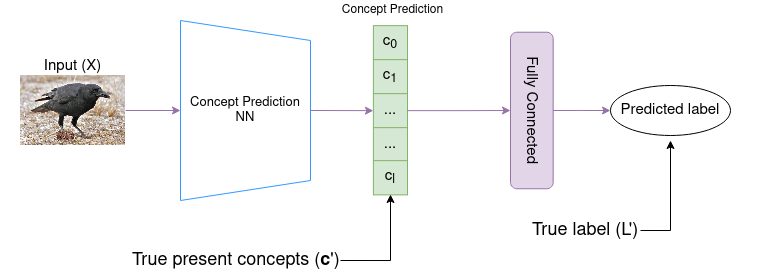
\includegraphics[width=\textwidth]{concept-bottleneck-pipeline/original-concept-bottleneck-model.png}
\label{original-concept-bottleneck}
\end{figure}

An end-to-end NN is transformed into a concept bottleneck one by forcing it to predict human-defined concepts before the final labels.
The final result of the model can then be interpreted by verifying the concepts used when making a decision.
For example, consider a bird prediction problem where human-defined concepts consist of the colour of the beak, wings and body.
If a bird is a crow, the model would predict that it has a black body, wings and beak before indicating that it is a crow.
From those results, an explanation \emph{The bird is a crow because it has black wings, black beak and black body} could be generated.

In this chapter, we take the concept bottleneck idea further.
We mine human-understandable concepts from text explanations of a label in place of a predefined set of concepts.
Such an approach would significantly simplify applying concept bottleneck pipelines in any domain.
It removes the need to predetermine an appropriate set of concepts and manually label all data points where they occur.
Text explanations, on the other hand, are sometimes readily available. For example, we could immediately use a patient's medical history report.
If the explanations are not readily available, they are easy to produce.


% Talk about Vikranth's work
\section{Inherited Work}
\label{inherited-work}

The work on the concept bottleneck pipeline has not been done from scratch.

This chapter itself is a continuation of the ideas proposed by Jeyakumar et al. in \emph{Automatic Concept Extraction for Concept Bottleneck-based Video Classification} \cite{RefWorks:RefID:16-2021automatic}. This paper failed to meet the acceptance threshold for the \href{https://iclr.cc/}{ICLR 2022} conference. 

The main contribution by Jeyakumar et al. is the \emph{Concept Discovery and Extraction Module} (CoDEx), a module that automatically uses explanations to extract text concepts.
That module has been applied to the MLB-V2E dataset, a baseball video dataset with explanations. \\
The architecture involving the \emph{Concept Discovery and Extraction Module} is shown in \ref{vikranth-concept-bottleneck}. 
In general, it is very similar to the standard architecture of the concept bottleneck architecture shown in \ref{original-concept-bottleneck} only with the CoDEx module replacing the true present concepts.

\begin{figure}[h]
\caption{Schematic representation of the concept bottleneck pipeline presented by Jeyakumar et al. (adapted from \cite{RefWorks:RefID:16-2021automatic})} 
\vspace{5pt}
\centering
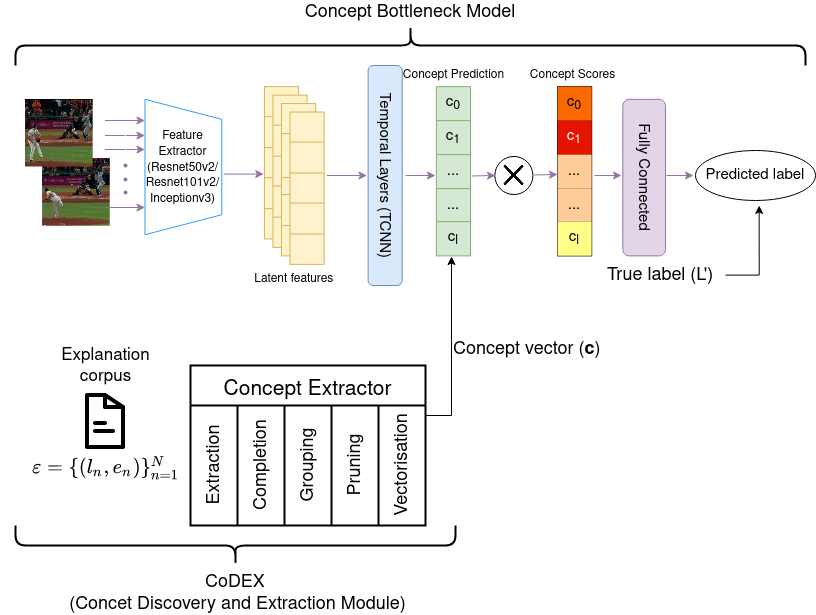
\includegraphics[width=\textwidth]{concept-bottleneck-pipeline/vikranth-concept-bottleneck.png}
\label{vikranth-concept-bottleneck}
\end{figure}


Jeyakumar et al. replace the set of human-crafted present concepts with the output of a CoDEx. 
In addition, to better understand each concept's impact on the final prediction, they add an attention layer after the concept layer to determine the concepts have more impact on the final prediction.
They extract the top three concepts with the highest attention score from that layer, which they use as explanations for a particular label. \\

\emph{Concept Discovery and Extraction Module} design is a vital element of the paper.
The CoDEx presented in the paper consists of 6 stages: \textbf{cleaning}, \textbf{extraction}, \textbf{grouping}, \textbf{completion}, \textbf{pruning}, and \textbf{vectorisation}. \\
The \textbf{cleaning} stage removes videos/explanations which are corrupted. \\
Using a constituency parser and a rule-based methodology, the \textbf{extraction} step determines if a portion of the phrase should be included as a candidate concept. 
The constituency parser uses the rules shown in the following table to extract concepts:

\begin{center}
\begin{tabular}{ |p{2cm}|p{12cm}|  }
 \hline
 \multicolumn{2}{|c|}{Rules determining whether a candidate concept should be included or excluded} \\
 \hline
 rule name & rule \\
 \hline
 Inclusion 1 & noun/pronoun → auxillary (optional) → particle (optional) → verb (optional) \\
 Inclusion 2 & noun/pronoun → auxiliary whose lemma is 'be' → any token \\
 Exclusion & subordinating conjunction \\
 
 \hline
 
\end{tabular}
\label{inclusion-exclusion-rules}
\end{center}

The \textbf{completion} stage looks up for concepts identified in some explanations while not other ones due to the behaviour of the constituency parser.
That stage is done by the substring lookup of existing concepts in all sentences. \\
The \textbf{grouping} step attempts to group concepts with similar meanings using agglomerative clustering \cite{RefWorks:RefID:13-mullner2011modern}.  \\
The \textbf{pruning} stage attempts to keep highly informative concepts by picking the smallest concept subset such that the mutual information \cite{RefWorks:RefID:30-mackay2004information} between the label and a concept vector does not fall below a certain percentage $\gamma$.
This problem is not solved precisely, but rather concepts are inserted using a greedy approach until the mutual information between the label and the newly constructed vector is not below a percentage $\gamma$. The authors chose $\gamma = 0.9$ as an appropriate value. \\
The vectorisation constructs the N x K concept matrix, where K is the number of concepts and N is the number of data points. 
The cell (n, k) is set to one if the concept k occurs for the data point n, zero otherwise.

After all these stages, a binary vector is produced for each data point, which is used in the NN training procedure.
Jeyakumar et al. train the neural network using the joint training approach, where they optimise for both the concept loss and final loss at the same time.
The concept loss is a binary cross entropy loss between a predicted concept vector and CoDEx produced true vector. In contrast, the final loss is a standard categorical cross entropy loss used for classification.

Using the CoDEx and the joint training procedure, the authors showed that their concept bottleneck pipeline had comparable performance to a standard end-to-end model.
In addition, the explanations they extracted were overwhelmingly better than the most common explanations.

% Changes we made to the concept bottleneck pipeline
\section{Adaptions to the Concept Bottleneck Pipeline}

In this chapter, we adapt the CoDEx part of the concept bottleneck pipeline to improve the performance and explainability of the entire model.

The \textbf{extraction} and the \textbf{completion} phase of the CoDEx have been removed from the pipeline.
The former used a rule-based approach to extract concepts.
The latter finds all concepts discovered by the constituency parser in one sentence but not in another using substring matching.

The removed stages are pretty and failed to account for a lot of information the video explanations conveyed.

To replace them extraction and completion we included \textbf{atomisation}, \textbf{generalisation} and \textbf{simple pruning} steps. \\
The chapter \ref{solving-nlp-tasks-logically} explains the first two stages (tasks) in great detail.
The \textbf{atomisation} stage splits provided sentences into one or more atomic sentences. 
Recall that the atomic sentences are sentences which an NLP expert cannot decompose into multiple valid sentences.
This procedure is done using hand-crafted interpretable rules, which are presented in the section \ref{solving-atomisation-task} along with the thought process for choosing the final solution.

The \textbf{generalisation} stage should extract all concept sentences from an atomic one. 
As explained in the section \ref{sentence-type-definitions}, the concept sentence is a syntactically correct sentence obtained by modifying a sentence's syntax tree.
To extract the concept sentences from an atomic sentence, we use a solution learned by ILASP, with the learning procedure described in \ref{solving-generalisation-task}.

The \textbf{simple pruning} stage, included between \textbf{generalisation} and \textbf{grouping} stage, is the simplest out of any of the steps present. 
It removes the concept if it fails to occur at least three times in the dataset.
The sole reason for including this stage is to speed up the subsequent steps because it slightly reduces the overall performance of the pipeline.
% INSERT reference to bird-flowers dataset
CoDEx pipeline for the bird-flowers dataset (\ref{applicability-in-other-domains}) takes less than an hour when the \textbf{simple pruning} stage is not included, which increases to over 10 hours without it.
This stage is only included when the CoDEx pipeline takes too long to compute otherwise because it is lossy.

The diagram summarising the new concept bottleneck pipeline is shown in figure \ref{full-architecture-diagram}.

% TODO: fix X in picture, add boxes for the three parts, missing outlining X as attention module
\begin{figure}[h]
\caption{The entire pipeline for the classification of the MLB-V2E dataset using the concept bottleneck model.} 
\centering
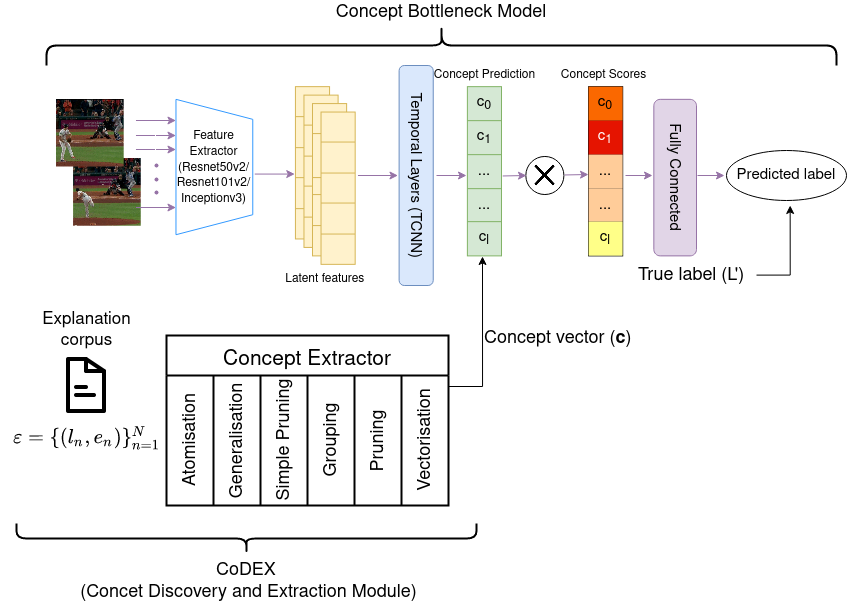
\includegraphics[width=\textwidth]{concept-bottleneck-pipeline/new-concept-bottleneck-pipeline.png}
\label{full-architecture-diagram}
\end{figure}

% INSERT Do cocnept bottlenecks learn as intended
There were recent concerns about the joint training procedure not truly accounting for concepts in their final predictions. 
So, we also attempt to use the sequential training procedure, isolating the training of concept and label prediction parts of the network.
Such a training procedure should perform similarly \cite{RefWorks:RefID:35-koh2020concept}, so we expect the similar results.

\section{Evaluation}

This section will discuss how well the newly presented CoDEx pipeline performs.
Any results produced will be compared with the previous iteration of the concept bottleneck pipeline and the uninterpretable end-to-end model, if applicable.
To keep concept bottleneck pipelines easily comparable, we prune the concepts such that only 78 of them remain.
This number was a desirable value for the original concept bottleneck pipeline \cite{RefWorks:RefID:16-2021automatic}.

Each concept bottleneck model is also trained using both joint and sequential models, unlike the \ref{inherited-work} which only uses the joint model.
% INSERT: Cite "do concept bottleneck models work as intended"
The difference between the two is that the joint optimises losses for both concepts and labels simultaneously, which sometimes overrules the nature of the concept bottleneck pipeline.
The sequential training model freezes the learned concept prediction layers, so the model must determine the final label from the concept predictions themselves.

% INSERT The caltech-ucsd birds-200-2011 dataset, Automated flower classification over a large number of classes
Also, we evaluate the concept bottleneck model on a new birds-flowers dataset, which combines randomly selected images from the CUB-200-2011 and 102 Category Flower Dataset along with their descriptions.
This evaluation inspects how well the concept bottleneck pipeline translates to different domains.

Finally, we will critically analyse the strengths and limitations of the implemented method and suggest areas for future improvement.

\subsection{CoDEx based evaluations}

% INSERT table into the appendix
Tables presenting concept strings for the old and new approaches and their occurrences are shown in Appendix X.

At first glance, both methods extract relevant concepts for the problem, although not all are perfect.
For example, the new method extracts a concept \emph{It was} which is not a relevant concept.
In general, the new method seems to extract concepts which better describe the labels, but we evaluate this belief concretely in this subsection.


\subsubsection{Measuring Cumulative MI}

% INSERT ref MacKay book; maybe insert Venn diagram from Wikipedia.  
Mutual Information $I(X;Y)$ \cite{RefWorks:RefID:30-mackay2004information} is defined as $I(X; Y) \equiv H(X) - H(X|Y)$. 
It estimates the average reduction in uncertainty about $x$ caused by understanding $y$'s value or vice versa. 
It is the average quantity of information conveyed by $x$ regarding $y$.

In the context of this project, the discrete variable $Y$ is a set of label outcomes. A possible outcome is a number between 0 and 4, where each number represents an event which occurred.
The discrete variable $X$ represents a set of extracted concepts with size $k$, where $k$ is a parameter tested in this evaluation.

In addition, given that the cumulative MI is under consideration, the set of size $k$ should ideally contain $k$ \emph{maximally informative} concepts, i.e. those which will result in the highest mutual information score.
However, finding such a set is infeasible as the problem is combinatorial \cite{RefWorks:RefID:16-2021automatic}. Still, we can get a highly informative set by greedily adding a single concept that improves MI the most. 

So, by measuring cumulative MI, we can determine how good the extracted concepts are at describing the labels.

The results can be seen in figure \ref{cummulative-mi-graphs}.

% TODO: replace this with a new version

\begin{figure}[h]
\caption{Cumulative MI graphs using old and new concept extraction pipeline}
\centering
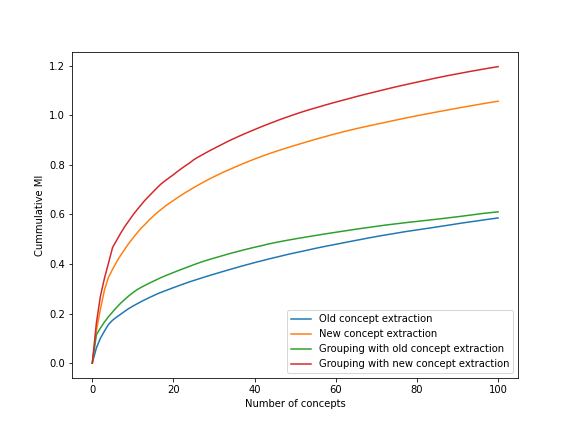
\includegraphics[width=\textwidth]{concept-bottleneck-pipeline/Cummulative MI graphs.png}
\label{cummulative-mi-graphs}
\end{figure}

% TODO: talk about specific numbers

It shows that the new concept extraction method drastically outperforms the old approach for the first 100 concepts.
Since only 78 are taken for the entire pipeline training, these results indicate that the new concept bottleneck performance should drastically improve.


\subsubsection{Concept Prediction Performance}

A corollary of the higher concept mutual information is a higher concept prediction accuracy.

Consider a classifier which would result in the highest possible accuracy for a dataset from binary vectors to labels.
Such a classifier assigns the correct label to any non-conflicting binary vector and the most common label to any conflicting binary vector. 
A conflicting vector is one whose outcome can result in multiple different labels.
The maximum possible accuracies are summarised in the table below:

\begin{center}
\begin{tabular}{ |M{3 cm}||M{3cm}|M{3cm}|  }
 \hline
 \multicolumn{3}{|c|}{Maximum accuracy comparison} \\
 \hline
 \hline
  & Old Concept Extraction&New Concept extraction\\ 
 \hline
 Training dataset & 51.1\% & 78.6\% \\
 Test dataset & 47.7\% & 87.7\% \\
 \hline
\end{tabular}
\end{center}

The highest possible accuracy with the new concept extraction for training and the test set is much greater than the values achievable with the old procedure.

To validate these results translate into practice, we train an MLP classification model from binary vectors to labels with both old and new concept extraction.
% INSERT reference RoBERTa
In addition, a RoBERTa transformer model is trained directly from an unedited human-generated explanation to estimate how much information is lost through concept extraction.
% INSERT: figure comparing transformer MLP with 
The results are presented in the figure \ref{from-concepts-accuracy-comparison}.

\begin{figure}[h]
\caption{Comparison of the label prediction performance from text with a transformer and predicted concepts using MLPs.}
\centering
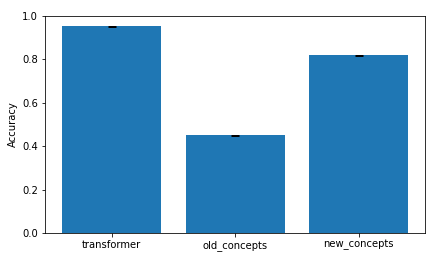
\includegraphics[width=0.5\textwidth]{concept-bottleneck-pipeline/from_explanations_accuracy_comparison.png}
\label{from-concepts-accuracy-comparison}
\end{figure}

These experiments convince us that the performance of a concept bottleneck performance should improve.
They also suggest that there is still room for improvement for the concept extraction since there is a 19\% accuracy improvement by training a model directly from the text.

\subsection{Performance of the Full Concept Bottleneck Pipeline}

The model performance is measured on the entire concept bottleneck pipeline.
We measure the final accuracy of the models with identical architectures using new and old concept extraction. 
In addition, the quality of the concept prediction is also measured as it can help understand whether the concept bottleneck nature of the model is indeed considered. \\
The precision metric is used to measure the concept prediction performance because detecting a subset of present concepts is often enough to determine the final label correctly.
Furthermore, most concept values are set to 0 for any data point, so metrics considering true negatives would have a high value even when the actual concept prediction is poor.
The final label prediction is measured using accuracy, as we want the predictions to be correct most of the time.
The predictive accuracies are also compared with an end-to-end model with an identical architecture, the highest value the concept bottleneck models could achieve.

The model accuracies are presented in the figure \ref{full-process-accuracy-comparison}.
\begin{figure}[h]
\caption{Comparison of the label prediction accuracy for NNs with no, old and new concept prediction in its intermediate layer. The graph on the right is the zoomed-in version of the one on the left to allow observing the differences in performance.}
\centering
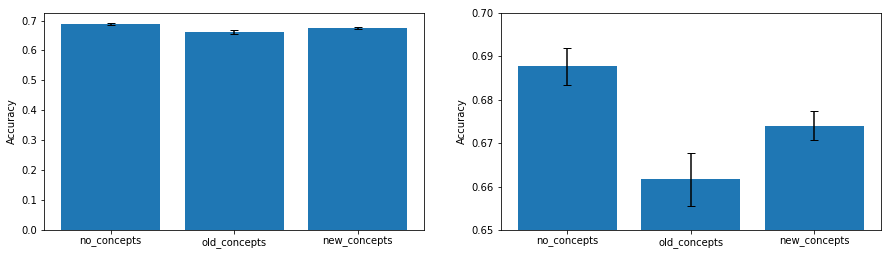
\includegraphics[width=\textwidth]{concept-bottleneck-pipeline/accuracy_comparison.png}
\label{full-process-accuracy-comparison}
\end{figure}

% TODO: analysis of the results
As expected, the model without concepts outperforms both concept bottleneck models. 
In addition, we expect that the new concept extraction outperforms the old one due to the higher mutual information value its concepts have. \\
However, we expected a much more significant performance difference between the concept bottleneck approaches due to a stark contrast in mutual information values.
To understand why that is the case, we need to consider the precision values of the concepts shown in \ref{full-process-concept-precision}.

\begin{figure}[h]
\caption{Comparison of the concept prediction precision score by a NN using old and new concepts in the intermediate layer.}
\centering
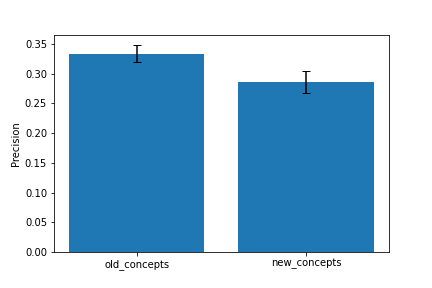
\includegraphics[width=0.5\textwidth]{concept-bottleneck-pipeline/concept_precisions.png}
\label{full-process-concept-precision}
\end{figure}

% TODO: analysis of the resutls
The concept predictions are extremely poor compared to the final results.
So, it is clear that concepts serve more as proxies for holding NN final prediction information instead of genuinely being learned by the network.
% INSERT Do concept bottleneck learn as intended.
This statement is backed up by the fact that old concept prediction even outperforms the prediction results directly from concepts, which would not have been possible in an actual concept bottleneck model (X).

To force the concept bottleneck nature of the model, we use the sequential training approach for the following experiments.
Such an approach first trains the concept prediction part of the network before training the network from concept predictions to final labels.

This approach results in the accuracy results shown in \ref{seq-full-model-results}.

\begin{figure}[h]
\caption{Comparison of the concept prediction precision score by a NN using old and new concepts in the intermediate layer.}
\centering
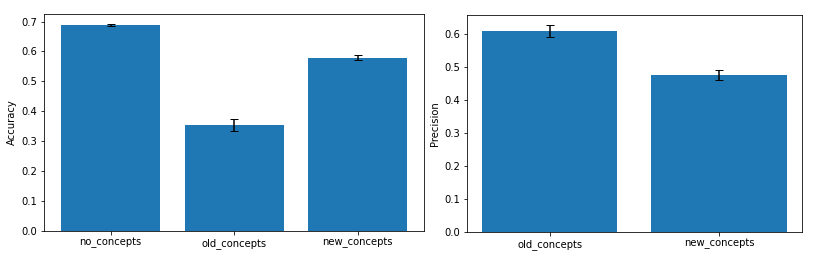
\includegraphics[width=\textwidth]{concept-bottleneck-pipeline/seq_comparison.png}
\label{seq-full-model-results}
\end{figure}

The sequential training has made the results closer to the expectation for the concept bottleneck model. 
There is a more significant difference between models using old and new concepts.
However, despite the concept prediction drastically improving the concept prediction results, they are still poor.
The precision values are still less than 0.5, whose improvement would greatly benefit the final performance too.

\subsection{Explainability of the Labels}

% INSERT appendix baseball rules quickly


The main reason we use the concept bottleneck pipeline is to allow interpretation of final labels using the intermediate concepts.
To do so, we compare the concept values after attention as human subjects prefer them over all alternatives in almost 70\% of the cases in \cite{RefWorks:RefID:16-2021automatic}.

We consider a concept as active for a data point if it has a score close to the maximum.
This behaviour was chosen because there was a sharp concept value drop of more than 50\% from the few top values, making these concepts lot less relevant for the final decision.


Unfortunately, due to a lack of resources, we have not been able to repeat the Mechanical Turk study done in \cite{RefWorks:RefID:16-2021automatic}. 
Instead, we only discuss three randomly selected test examples and qualitatively compare the old and new concept predictions for them: \\


% Label 1: curr_point = 78, id: KP4EFXZPM12B
Sourced explanation 1: \emph{The batter swung the bat and hit it into foul territory. This was called a foul ball by the ump}. \\
True label 1: foul.

The results are shown in \ref{concepts-results-1}.
The video consisted of a batter hitting the ball hitting a ball in the air behind him in the foul territory.
Both networks accurately predict this sequence as a foul.

\begin{figure}[h]
\caption{Most relevant concepts for example 1 along with their concept scores. The LHS shows the ones predicted by the old concept bottleneck, while the RHS is predicted by the new one.}
\centering
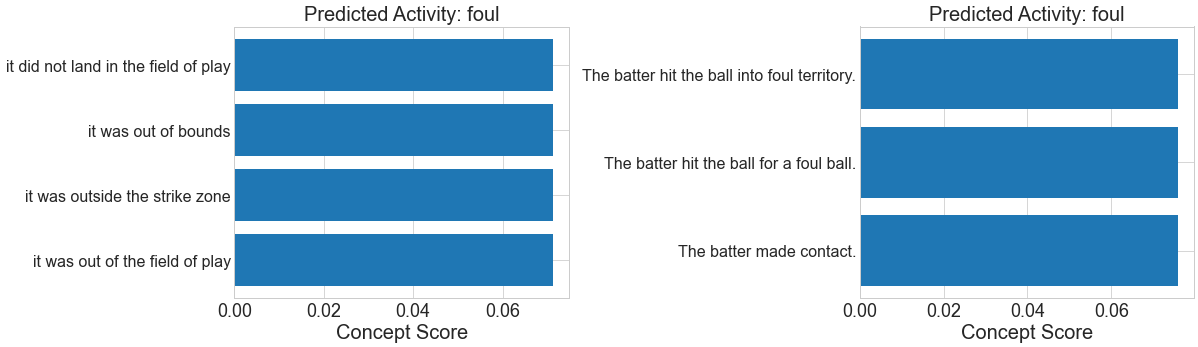
\includegraphics[width=\textwidth]{concept-bottleneck-pipeline/explanations_concepts1.png}
\label{concepts-results-1}
\end{figure}

For the new concept bottleneck network, all predicted concepts are correct.
The batter has indeed made contact, the ball went into the foul territory and was indeed a foul ball.
They describe well all the events that happened.
On the other hand, old concepts also perform well in this case.
One should be able determine that the final label should be foul from the concepts. 
The concept \emph{it was outside of strike zone} is wrong. 
If that piece of information is indeed correct, the true label would have been ball instead of the foul.
In addition, \emph{it was out of bounds}, \emph{it did not land in the field of play}, \emph{it was out of field of play} all capture the same piece of information.
That the ball landed outside of the allowed territory.
It may be sufficient to only present one such concept.

Although both concepts are good enough to accurately predict the final label, the new one would usually be preferred.
It is not only because the old concept bottleneck presents an incorrect sentence, but also because the new concepts seem much clearer.
The user does not need to infer what "it" is referring to. \\

% Label 2: curr_point = 122, id: SAGXX461QCAB
Sourced explanation 2: \emph{The batter hit it in play and it was not caught.} \\
True label 2: play

\begin{figure}[h]
\caption{Most relevant concepts for example 2 along with their concept scores. The LHS shows the ones predicted by the old concept bottleneck, while the RHS is predicted by the new one.}
\centering
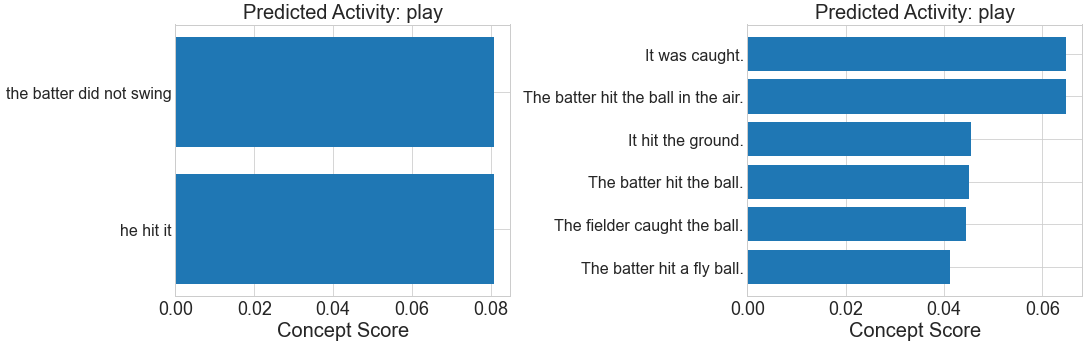
\includegraphics[width=\textwidth]{concept-bottleneck-pipeline/expalantions_concepts2.png}
\label{concepts-results-2}
\end{figure}

The results are shown in \ref{concepts-results-2}.
The video in explanation 2 showed a batter hitting a fly ball which an outfielder caught after it hit the ground.
Both networks accurately predict this sequence as an play.

Unlike the previous video, the final label would not clearly be determined by both explanations.
The old concept prediction only predicted two conflicting concepts out of which only \emph{he hit it} is correct.

On the contrary, the new concept extraction predicted all relevant events that have occurred in the video.
These concepts do have some redundancy, such as \emph{It was caught} and \emph{The fielder caught the ball} presenting the same thing.
Moreover, the new concepts showcase finer level of granularity in event prediction by predicting that a fly ball has occurred. 
The concept scores might slightly confuse a user, in this case, as they highlight two concepts more than the others. 
If these were showcased on their own, they would seem more related to \textit{out} rather \emph{play}. \\

% Label 3: curr_point = 201, id: ZLP8NFBVSNHS, strike
Sourced explanation 3: \emph{the batter did not swing at a ball in the strike zone}. \\
True label 3: strike

The results are shown in \ref{concept-results-3}.
Both networks correctly predict this sequence as a strike.

\begin{figure}[h]
\caption{Most relevant concepts for example 3 along with their concept scores. The LHS shows the ones predicted by the old concept bottleneck, while the RHS is predicted by the new one.}
\centering
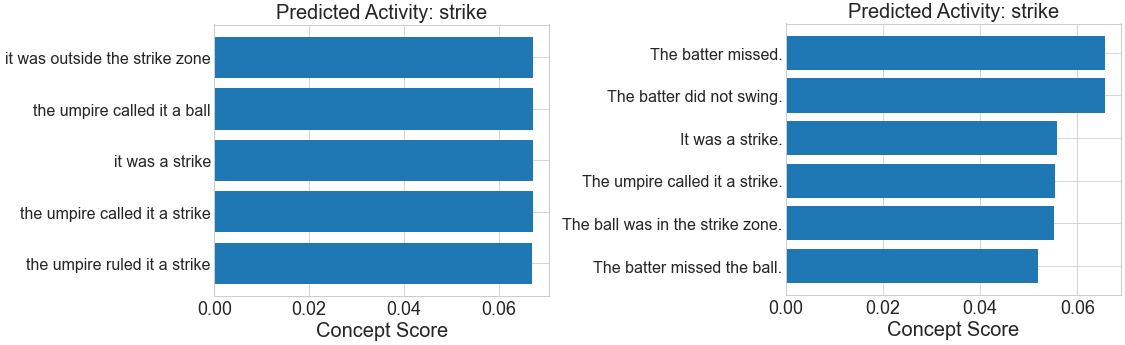
\includegraphics[width=\textwidth]{concept-bottleneck-pipeline/explanations_concepts3.png}
\label{concept-results-3}
\end{figure}

Again, the new concept extraction pipeline seemed to have extracted better for describing the label.
There are two reasons for it: they are more accurate and they they describe multiple events from which the final label could be inferred.

The old concept prediction pipeline predicted two incorrect concepts: \emph{it was outside of the strike zone} and \emph{the umpire called it a ball}.
All of the newly inferred concept are correct, on the contrary.

The new concept prediction describes multiple relevant events. 
For example, it describes both the umpire ruling the event as a strike and the ball being in the strike zone.
On the other hand, only the umpire calling the pitch a strike was predicted. 
The other two concepts either describe exactly the same thing \emph{the umpire ruled it a strike} or have predicted the final label instead of a concept \emph{it was a strike}.
Note that the latter was also predicted in the new concept bottleneck pipeline. 
That sentence should be omitted since it would be a meaningful statement in any explanation describing why the label occurred. \\

To sum up, there seems to be promise that the new method improves explanations in both accuracy and the level of detail.
We should create a human study in the future to validate these claims.
In addition, notice that the current the current set of explanations, although mostly good, would not be considered true present concepts by the CoDEx module.
They would need to occur in the explanation for that to be the case.

In addition, notice that a few of concepts chosen should not actually be predicted since they do not occur in the explanation.
However, they were mostly correct, especially for the new concept extraction.
So, the poor precision value may not not necessarily hurt explanations, but rather correct concepts may not often be captured by the CoDEx module.

\subsection{Applicability in other Domains}
\label{applicability-in-other-domains}

% TODO: finish

As argued, the idea presented in this section in theory is not tied to video applications.
% INSERT The caltech-ucsd birds-200-2011 dataset, Automated flower classification over a large number of classes, if I can reference descriptions
In this evaluation, we measure how well does the CoDEx module fare when applied to a birds-flowers dataset.
This dataset consists of 2000 birds/flowers images taken from X and X, combined with image descriptions generated for these respective datasets.
As such, the explanations are written such that they describe the image, rather than the label.
% INSERT ref results compared to 
It was chosen due to its simplicity for standard NN, as demonstrated by the high accuracy of a non-concept bottleneck model in X.
In addition, the explanations were also readily available to use for concept prediction.

Simply observing the concept we see that the set of concepts extracted may be applicable quite well.
For example, the CoDEx extracts the following concepts together with their occurrence in the dataset:
\begin{verbatim}
The bird has feathers. % 18
This flower has pistil. % 18
\end{verbatim}
Despite the sentence structure immediately highlighting whether it is a bird or a flower, the model would nevertheless try to learn what are feathers and what are pistils.
The issue is the count occurrence for doing so.
Clearly, more than 18 birds in the dataset have feathers, and more than 18 flowers have pistils.
This poor count is a result of label explanations extracted from the two label descriptions focusing on differences between different species of birds/flowers instead of the differences between the two.
In addition, not all concept are useful, such as \emph{This bird has}, but in general there seems to be enough information to determine the final labels correctly.

On the other hand, the concepts produced by the old approach seem much worse. 
It is often quite unclear which label they correspond to, such as \emph{that are oval shaped}.
Or, there is a few very specific concepts which are grouped together of other long concepts.
For example, a concept \emph{this is a white and black bird with a black crown and a long black beak} would fall into that category.

All the extracted concepts are included in Appendix X, along with frequencies of concept occurrence.

To validate whether the initial observations translate to tangible results, we evaluate how well can an MLP predict the final result.
The input to will concept prediction vectors produced by old and new CoDEx modules.
% INSERT reference RoBERTa
To estimate how much information is lost by mining concepts, the results are compared against a fine-tuned RoBERTa transformer trained directly from text.

\begin{center}
\begin{tabular}{ |M{4cm}||M{3cm}|M{3cm}|M{3cm}|  }
 \hline
 \multicolumn{4}{|c|}{Results from explanations only} \\
 \hline
 & Transformer & Old concepts & New concepts \\
 \hline
 Final accuracy & 1.000 $\pm$ 0.000 & 0.844 $\pm$ 0.008 & 0.874 $\pm$ 0.006 \\
 \hline
\end{tabular}
\end{center}

The newly extracted concepts are able to better distinguish between labels, although the difference is not as big as for the baseball dataset.
The main reason for a loss in accuracy is the case where all inputs are 0, where any concept that was detected was pruned.
This case happens more often for the old concept extraction, but the new one is not immune.
As the transformer has the perfect accuracy, it is clear that its is extremely easy to distinguish between the two labels from descriptions.

% TODO: model architecture
We further evaluate the jointly trained models with identical architecture and hyper-parameters using old, new or no concepts in the intermediate layers:

\begin{center}
\begin{tabular}{ |M{4cm}||M{3cm}|M{3cm}|M{3cm}|  }
 \hline
 \multicolumn{4}{|c|}{Full model results} \\
 \hline
 & No concepts & Old concepts & New concepts \\
 \hline
 Final accuracy & 0.979 $\pm$ 0.004 & 0.987 $\pm$ 0.002 & 0.989 $\pm$ 0.002 \\
 Concept precision & / & 0.367 $\pm$ 0.021 & 0.212 $\pm$ 0.009 \\
 \hline
\end{tabular}
\end{center}

The final accuracies of the models all have similarly high values, which is desirable.
However, the concept precision results are poor, similar, but slightly worse, to the results for the MLB-V2E \cite{RefWorks:RefID:16-2021automatic} dataset.
As mentioned, the text explanations do not describe all features that a bird/flower has.
The CoDEx pipelines for that reason often fail to account for lots of concepts present in the image but not the explanations during training.
In addition, the reason behind higher concept accuracy may be related to the NN optimising for a positive concept value much more often with new concept extraction.
The training set for the new concept bottleneck pipeline has more than twice the number of detected concepts.

We further present the predicted concept values for randomly selected data-points shown in figure \ref{bird-concept-predictions} and \ref{flower-concept-predictions}.

\begin{figure}[h]
\caption{Most relevant concepts for the image shown below along with their concept scores. The LHS shows the ones predicted by the old concept bottleneck, while the RHS is predicted by the new one.}
\centering
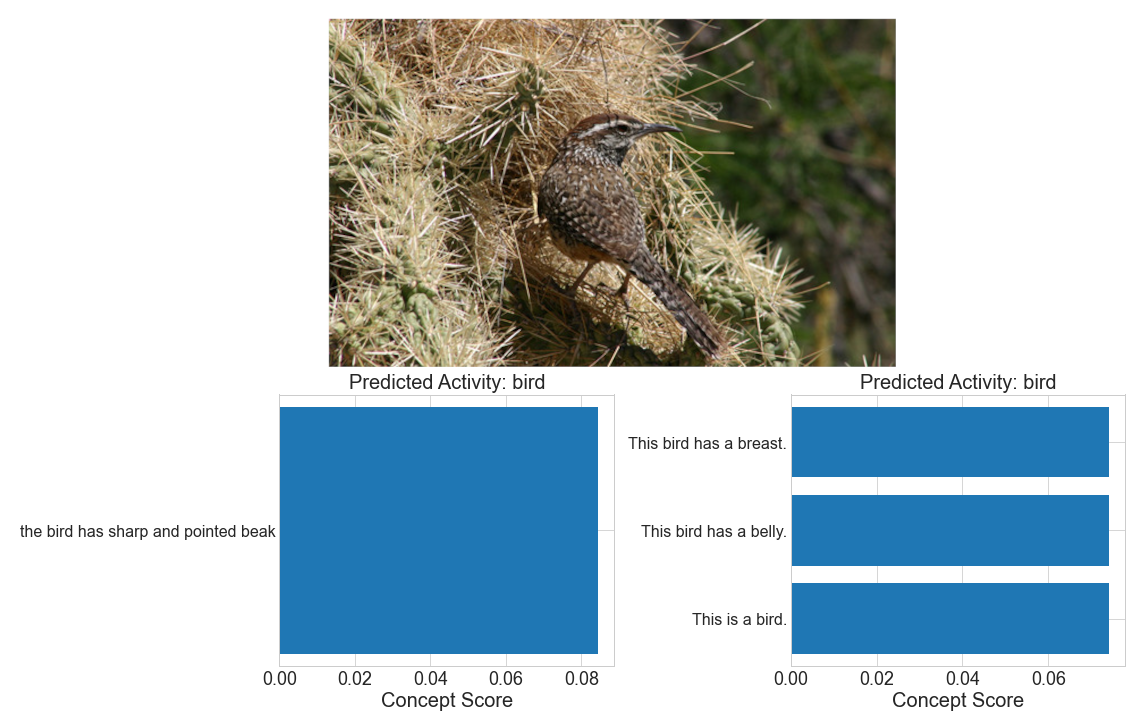
\includegraphics[width=\textwidth]{concept-bottleneck-pipeline/birds_predictions.png}
\label{bird-concept-predictions}
\end{figure}

For the bird example in \ref{bird-concept-predictions}, both outcomes are could be better.
The old concept bottleneck pipeline only shows a true but very specific feature.
On the other hand, the new concept bottleneck pipeline predicted better concepts that would describe some bird well.
However, given the orientation of the bird in the image, specifying that it has a breast and belly seems counter-intuitive.

\begin{figure}[h]
\caption{Most relevant concepts for the image shown below along with their concept scores. The LHS shows the ones predicted by the old concept bottleneck, while the RHS is predicted by the new one.}
\centering
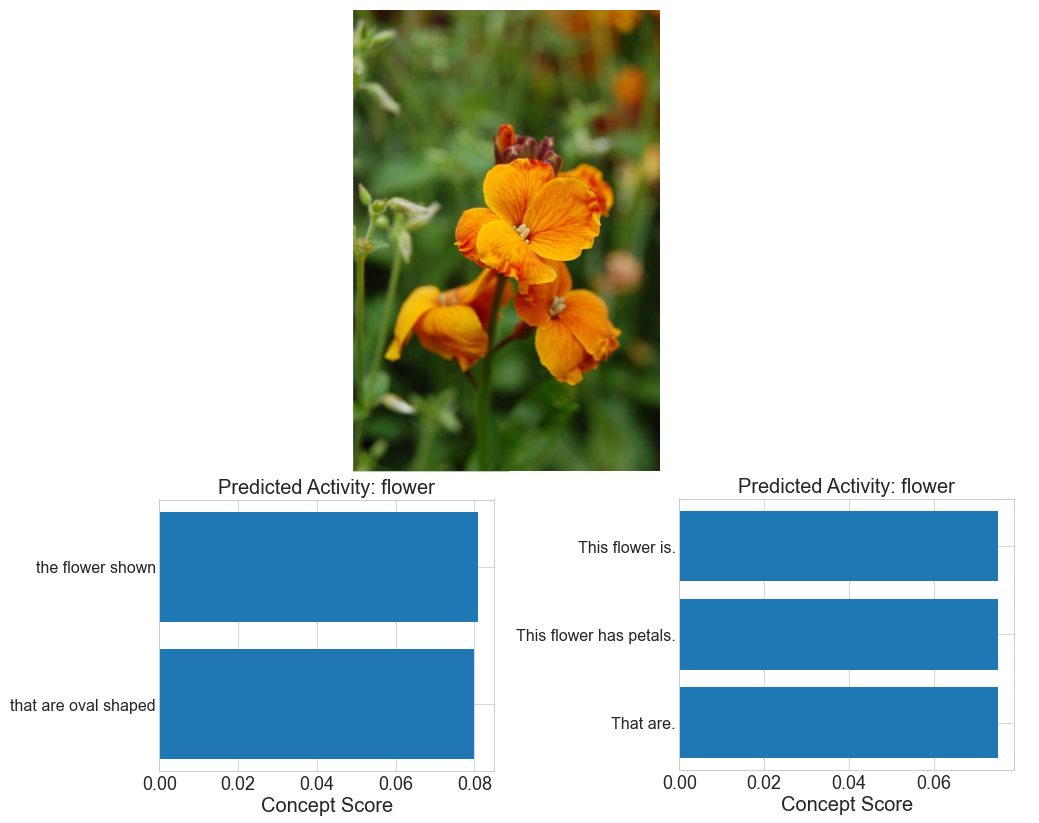
\includegraphics[width=\textwidth]{concept-bottleneck-pipeline/flower_predictions.png}
\label{flower-concept-predictions}
\end{figure}

The results for the \ref{flower-concept-predictions} are could be better.
The new concept bottleneck extracts well that \emph{this flower has petals}.
However, the other two concepts are not even valid sentences.
The old concept bottleneck similarly extract concept texts missing crucial information.


To sum up, neither method extracts good concepts for the bird-flowers dataset.
The conjunction of bird image and flower descriptions .
We believe that for the method to work, the explanations need to be generated such that they highlight why this data-point should be assigned to exactly this class and not the other.


\subsection{Conclusion}

In this chapter, we show that the addition of atomisation and generalisation greatly helps the concept bottleneck pipeline performance.
When incorporated into the concept bottleneck pipeline, the new CoDEx has much higher mutual information,  predictive accuracy, and performance.
In addition, there is an indication that its explanation generation is much better.

We also highlight a possible issue with joint training of a concept bottleneck model that may not truly consider the concept bottleneck nature of the problem.
However, to achieve comparable performance with the sequential training, we need to find a way to capture all the concepts that occur in the video.

\chapter{Logic-Based Classification}
\label{logic-based-classification}

% TODO: Alessandra feeedback
% Concept extraction can be used for a classification problem - that problem uses attention on the concepts to determine which ones are more active
% A more interpretable approach would involve rule-based classification, which we explore in this section
% Furthermore, despite the concept extraction from text presented, concepts can really be any features which is accounted for in this chapter.

In order to find reasons for choosing a particular label, the concept bottleneck pipeline \cite{RefWorks:RefID:35-koh2020concept} uses human-explainable high-level concepts in the intermediate layer.
These concepts should help a user to understand why a prediction happened.
However, just because concepts are predicted does not mean they are indeed used in the final prediction.

For example, a network may learn a pattern which predicts a label \emph{out}, if some concept has a value greater than 0.2.
Yet, such a concept would not be shown to the user as relevant for the final prediction.
Showcasing concepts after the attention layer, as we have done in the previous chapter, would showcase more relevant concepts for the final prediction.
Still, the attention layer showcases how much weight each concept has in the final prediction, but not the logic the MLP uses in order to choose the final label.

A fully interpretable method for predicting the final label would provide a clear link between the concepts and the outcomes.
In addition, model from concepts to the label can be validated and should in an ideal case follow the same logic as humans.

To improve upon the concept bottleneck model interpretability, this chapter presents a classification method using an ILP system.
The method works with probabilistic facts, allowing it to be incorporated into a concept bottleneck pipeline (Chapter \ref{concept-bottleneck-pipeline}).
Nevertheless, it is not limited to text concepts; it is applicable with any interpretable probabilistic NN output. 
% INSERT ref to evaluation
In section X, we use it with outcomes of a image classification task.
The ILP system utilised for this task is FastLAS \cite{RefWorks:RefID:19-law2020fastlas:}, a scalable system that incorporates criteria for domain-specific optimisation.

% TODO: change title
\section{Change to the Concept Bottleneck Architecture}
\label{change-to-the-concept-bottleneck-architecture}

An introduction of the rule learning component would result in the change in the concept bottleneck architecture shown in figure \ref{logic-based-concept-bottleneck}.
\begin{figure}[h]
\caption{A flowchart to select an outcome of a multi-label classification problem.}
\vspace{10pt}
\centering
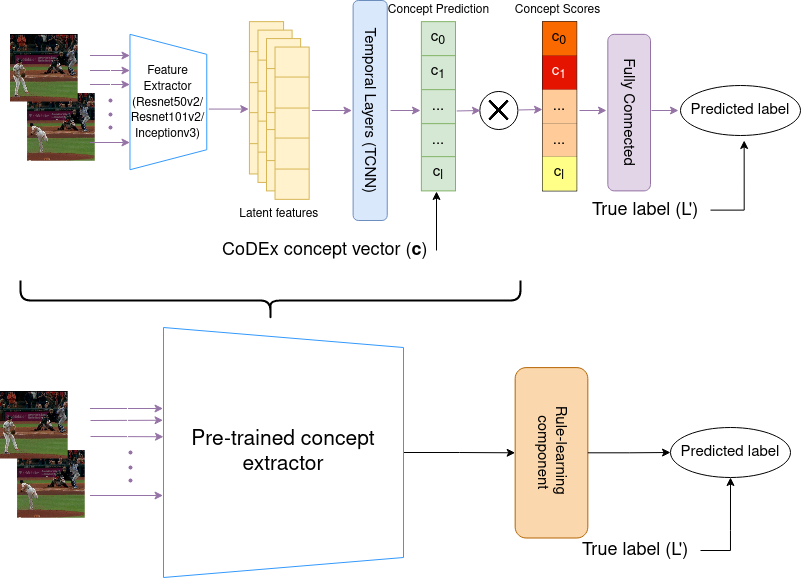
\includegraphics[width=\textwidth]{logic-based-classification/logic-based-classification-architecture.png}
\label{logic-based-concept-bottleneck}
\end{figure}

Training a concept bottleneck pipeline then turns into a 3-step process:
\begin{enumerate}
    \item Train a model in the same manner as in the Chapter \ref{concept-bottleneck-pipeline}, by minimising the loss CoDEx concept vector and final label prediction loss.
    \item Generate examples for the rule-learning component using the concepts predicted by the model from step 1). Each example needs to take into account the probabilities of all concepts.
    \item Train the rule-learning component.
\end{enumerate}

At run-time take predict the concepts using the model trained in step 1, before applying the rules learned in step 3 to obtain the final prediction.

% INSERT FF-NSL reference
The ILP paradigm does not support any notion of probability; an atom can either be in or out of an answer set. 
So, to force the learner to treat less less likely cases differently, we carefully choose the FastLAS example penalties, similar to X.
However, we aim to use those penalties to find the most likely solution.

\section{Choosing FastLAS Parameter Values}
\label{choosing-fastlas-parameter-values}

% INSERT reference to background section decomposable
FastLAS can find an optimal solution with respect to a scoring function of kind ($\curly{S} + \curly{S}_{pen}$), where $\curly{S}$ is a decomposable scoring function (X) and $\curly{S}_{pen}$ is a sum of all uncovered example penalties.

In this section, we attempt to find the appropriate scoring function $\curly{S}$ and values for penalties such that the final solution is highly likely given the learning task tuple $T = \langle B, M, E_{prob} \rangle$. 

\subsection{Used Notation}

Let our set of examples $E_{prob}$ be $\{(\vec{x}_e, y_e)\}_{e=1}^{E} \in \curly{E}$ with $E$ examples. 
An example $(\vec{x}_e, y_e)$ consist of a vector of concept probabilities $\vec{x}_e = (x_{ec})_{c=1}^C$ and a label $y_e \in \curly{L}$ assigned to the example $e$ from the set of possible labels $\curly{L}$.
The symbol $x_{ec}$ denotes a priori probability that concept $c$ takes truth value (=1) in example $e$.
Moreover, $C$ is the number of extracted concepts for a given problem. \\
We can represent examples as a matrix of concept probabilities.  
The examples can be represented as an input matrix of concept probabilities $\vec{X} = (\vec{x}_e^T)_{e=1}^E$ and an output vector of target labels $\vec{y} = (y_e)_{e=1}^E$.

Let $\curly{H}$ be the set of all possible hypotheses. The term $p(y_e|H, \vec{x}_{e})$ represents the probability that the example $e$ is covered, for any hypothesis $H \in \curly{H}$,


We introduce notation for grounded examples, as answer sets can only contain grounded atoms.
A grounded example $(\vec{z}_e, y_e)$ is an example where each concept $c$ in an example $e$ is assigned a truth value $z_{ec} \in \{0,1\}$ (integer form). 
The term $\vec{z}_e = (z_{ec})_{c=1}^C \in \curly{Z}_e$  is a binary vector representing the ground assignment. 

\subsection{Determining Optimal Example Penalties}

We want to choose the example penalties such that the FastLAS output hypothesis $H$ is the maximum-likelihood hypothesis $H_{\text{ML}}$, i.e. the output hypothesis should satisfy the following equation:
\begin{align}
H_{\text{ML}} = \arg\max_{H}
p(\vec{y}|H, \vec{X})
\end{align}

Making an assumption that given a model and concept probabilities, the labels for any two examples are conditionally independent we can rewrite the term $p(\vec{y}|H, \vec{X})$ in the following manner:
\begin{align}
p(\vec{y}|H, \vec{X})
= \prod_{e} p(y_e|H, \vec{x}_e) \label{eq6.3}
\end{align}


As the $ln = log_e$ function is monotonically increasing in the range $(0, \infty)$ and as the above equation produces values in that range, it is equivalent to maximising the $ln$, resulting in the following optimisation target:
\begin{align}
H_{\text{ML}}
& = \arg\max_{H}
\ln p(\vec{y}|H, \vec{X}) \nonumber \\
& = \arg\max_{H}
\sum_{e} \ln p(y_e|H, \vec{x}_e) && \text{(by \ref{eq6.3})} \nonumber \\
& = \arg\min_{H}
-\sum_{e} \ln p(y_e|H, \vec{x}_e) && \text{(alternative objective)} \label{ex6.4}
\end{align}


% TODO: define Z
We can now calculate the probability that a label $y_e$, for example $e$, is covered by a hypothesis $H$ where we know the set of concept probabilities $\vec{x}_e$.
That probability is computed by considering all possible grounding that $\vec{x}_e$ induces.
It is given by:
\begin{align}
p(y_e|H, \vec{x}_e)
& = \sum_{\vec{z} \in \curly{Z}_e} p(y_e, \vec{z} | H, \vec{x}_e) && \text{(sum rule)} \nonumber \\
& = \sum_{\vec{z} \in \curly{Z}_e} p(y_e | \vec{z}, H, \vec{x}_e) p(\vec{z} | H, \vec{x}_e) && \text{(conditional probability)} \nonumber \\
& = \sum_{\vec{z} \in \curly{Z}_e} p(y_e | \vec{z}, H) p(\vec{z}| \vec{x}_e) && \text{(by independence)} \nonumber \\
& = \expct_{\vec{z} \sim p(\vec{z}| \vec{x}_e)}[p(y_e|\vec{z},H)] \label{ex6.5}
\end{align}

Considering the $\ln$ of the term above, we can use the Jensen's inequality to push it inside the expectation:
\begin{align}
\ln p(y_e|H, \vec{x}_e)
&= \ln \expct_{\vec{z} \sim p(\vec{z}| \vec{x}_e)}[p(y_e|\vec{z},H)] \nonumber \\
&\leq \expct_{\vec{z} \sim p(\vec{z}| \vec{x}_e)}[\ln  p(y_e|\vec{z},H)] 
\nonumber \\
\end{align}

We further assume that the bounds of Jensen's inequality are sufficiently tight, i.e. we assume that:
\begin{align}
\ln p(y_e|H, \vec{x}_e)
&\approx \expct_{\vec{z} \sim p(\vec{z}| \vec{x}_e)}[\ln  p(y_e|\vec{z},H)] \label{jensen-approx}
\end{align}

Now we can estimate the expectation by sampling $I$ ground examples for example $e$, where ground examples are $\vec{z}_{i} \sim p(\vec{z}| \vec{x}_e)$, then:
\begin{align}
\expct_{\vec{z} \sim p(\vec{z}| \vec{x}_e)}[\ln  p(y_e|\vec{z},H)]
\approx \frac{1}{I} \sum_{i=1}^{I} \ln  p(y_e|\vec{z}_i,H) \label{sampling-result}
\end{align}


For some hypothesis, $H\in \curly{H}$, a grounded example is or is not covered by $H$. We allow a label to be incorrect with some small error $\epsilon > 0$, resulting in the following probabilistic interpretation:
\begin{align}
p(y_e | \vec{z}, H) =
\begin{cases}
1 - \epsilon & \text{if } H, \vec{z} \models y_e \\
\epsilon & \text{otherwise}
\label{def-ground}
\end{cases}
\end{align}

Combining all the results presented, we can derive the following:
\begin{align}
H_{\text{ML}}
& = \arg\min_{H} 
-\sum_e \ln \left( \expct_{\vec{z} \sim p(\vec{z}| \vec{x}_e)}[p(y_e|\vec{z},H)] \right ) 
&& \text{(by \ref{ex6.4} and \ref{ex6.5})} \nonumber \\
& \approx \arg\min_{H}
-\sum_e \expct_{\vec{z} \sim p(\vec{z}| \vec{x}_e)}[\ln \left[ p(y_e|\vec{z},H) \right ]]  
&& \text{(by \ref{jensen-approx})} \nonumber \\
& \approx \arg\min_{H}
\sum_e \frac{1}{I} \sum_{i=1}^I -\ln \left[ p(y_e|\vec{z},H) \right ]
&& \text{(by \ref{sampling-result})} \nonumber \\
& = \arg\min_{H} \sum_e \frac{1}{I} \sum_{i=1}^I  \left(-\ln  [p(y_e|\vec{z}_{ei},H)] + \ln (1-\epsilon) \right)
&& \text{(constant shift)} \nonumber \\
& = \arg\min_{H}
\sum_e \frac{1}{I} 
\left (
\sum_{H,\vec{x}_{ei}\models y_e} 0
+
\sum_{H,\vec{x}_{ei}\not\models y_e} (-\ln \epsilon + \ln (1 - \epsilon))
\right ) 
&& \text{(by \ref{def-ground})} \nonumber \\
& = \arg\min_{H}
\sum_e  
\sum_{H,\vec{x}_{ei}\not\models y_e} -\frac{1}{I}\ln \left ( \frac{\epsilon}{1 - \epsilon} \right ) \label{eq-final-no-int}
\end{align}


Optimising only for the $\curly{S}_{pen}$, FastLAS would return the following solution:
\begin{align}
H
& = \arg\min_{H}
\sum_e  
\sum_{H,\vec{x}_{ei}\not\models y_e} e_{pen}
\end{align}

Hence, by setting the penalty for each example to $-\frac{1}{I} \ln \left ( \frac{\epsilon}{1 - \epsilon} \right )$ and prior penalties to 0, FastLAS would return a solution close to the maximum likelihood for all examples.

\subsubsection{Integer penalties}
\label{integer-penalties}

FastLAS does not support any floating point number calculations, including penalty values.

But, we can overcome this issue.
Let us consider a large value $K \in \reals^+$, and then round $K$ multiplied by each term in the sum to the nearest integer. Because for large enough $K$:
\begin{align}
    Kt \approx round(Kt) \label{rounding}
\end{align}

In addition, minimising any $t \in \reals^+$ is equivalent to minimising $K t$ for any $K \in \reals^+$.
So, the function we wish to minimise becomes: 
\begin{align}
H_{\text{ML}}
& = \arg\min_{H}
\sum_e  
\sum_{H,\vec{x}_{ei}\not\models y_e} -\frac{1}{I}\ln \left ( \frac{\epsilon}{1 - \epsilon} \right ) 
&& \text{(\ref{eq-final-no-int})} \nonumber \\
& = \arg\min_{H}
K \sum_e  
\sum_{H,\vec{x}_{ei}\not\models y_e} -\frac{1}{I}\ln \left ( \frac{\epsilon}{1 - \epsilon} \right ) 
&& \text{(scaling $t \in \reals^+$ by $K \in \reals^+$)} \nonumber \\
& = \arg\min_{H}
\sum_e  
\sum_{H,\vec{x}_{ei}\not\models y_e} -\frac{K}{I}\ln \left ( \frac{\epsilon}{1 - \epsilon} \right ) \nonumber \\ 
& = \arg\min_{H}
\sum_e  
\sum_{H,\vec{x}_{ei}\not\models y_e} \text{round} \left ( -\frac{K}{I}\ln \left ( \frac{\epsilon}{1 - \epsilon} \right ) \right )
&& \text{(by \ref{rounding})}
\end{align}

Therefore, after choosing some large $K > 0$, we assign the non-coverage penalty of $\text{round} \left ( -\frac{K}{I} \ln \left ( \frac{\epsilon}{1 - \epsilon} \right ) \right )$ for each example.

\subsection{Incorporating a Prior over the Hypothesis Space}

Now, we can extend the approach done in the previous section by considering a prior over hypothesis space ($p(H)$) too.
The extension would give a plausibility value to each potential $H$ before we evaluate its fitness on the examples. 
We can combine this with the likelihood function to give a posterior probability for the data and hypothesis, namely:
\begin{align}
p(\vec{y}, H|\vec{X})
& = p(\vec{y}|H, \vec{X})p(H)
\end{align}

We can log this to get:
\begin{align}
\ln p(\vec{y}, H|\vec{X})
& = \ln p(\vec{y}|H, \vec{X}) + \ln p(H)
\end{align}

Maximising the above equation leads to what we would call the maximum posterior estimate for $H$, or maximum a posteriori (MAP) estimate:
\begin{align}
H_{\text{MAP}}
& = \arg\max_{H} \ln p(\vec{y}|H, \vec{X}) + \ln p(H) 
\end{align}

% As with the maximum likelihood approach we can maximise the rescaled expression using $K \in \reals^+$ giving:
% \begin{align}
% h_{\text{MAP}}
% & = \arg\max_{h} \left(K\ln p(\vec{y}|h, \vec{X}) + K\ln p(h) \right)
% \end{align}

% Or we can see this as minimising a negative log-loss:
% \begin{align}
% h_{\text{MAP}}
% & = \arg\min_{h} \left(-K\ln p(\vec{y}|h, \vec{X}) - K\ln p(h) \right)
% \end{align}

% Note the important point here is that the scale of the penalties on the prior must match the scale of penalties on the examples.

\subsubsection{Choosing a Meaningful Prior over the Hypothesis Space}

There are several ways to place a prior on hypothesis space. 
The default ILASP \cite{RefWorks:RefID:18-law2020ilasp} and the usual FastLAS approach assign smaller penalties, i.e., higher prior probabilities, to shorter clauses.
% INSERT online symbolic learning of policies for explainable security
Some problems benefited from assigning lower penalties to "ideal length" rules, such as X.

We have opted for a slightly different approach. \\
Starting with a set of potential rules $\curly{R}$, let $q_r$ be an independent probability that $r$ is included in $H$ (written $r \in H$) for every potential rule $r \in \curly{R}$. Then the prior is written as:
\begin{align}
p(H) = \left(\prod_{r \in H} q_r\right)\left(\prod_{r \in \curly{R}\setminus H} (1-q_r)\right)
\end{align}

We can log this for convenience:
\begin{align}
\ln p(H) = \sum_{r \in H} \ln q_r + \sum_{r \in \curly{R}\setminus H} \ln(1-q_r) \label{log-prior-rule}
\end{align}


For a fixed reference hypothesis such as $H_0 = \emptyset$, maximising the posterior is equivalent to maximising the posterior divided by the prior, resulting in:
\begin{align}
H_{\text{MAP}}
& = \arg\max_{H} p(\vec{y}|H, \vec{X}) p(H)  \nonumber \\
& = \arg\max_{H} \left(\frac{ p(\vec{y}|H, \vec{X}) p(H)}{p(H_0)}\right)  \nonumber \\
& = \arg\min_{H} \left( -K\ln p(\vec{y}|H, \vec{X}) - K \ln \frac{p(H)}{p(H_0)}\right) \label{h-map-final}
\end{align}
The above equation holds for some $K > 0$, added to deal with FastLAS inability to work with non-integers as in \ref{integer-penalties}.

The ratio of the overall change in prior for any hypothesis $H \in \curly{H}$ from the empty hypothesis $H_0 = \emptyset$ can then be calculated using \ref{log-prior-rule} as follows:
\begin{align}
\ln \left(\frac{p(H)}{p(H_0)}\right) 
& = \sum_{r \in H} \ln q_r + \sum_{r \in \curly{R}\setminus H} \ln(1-q_r) \nonumber
- \sum_{r \in \emptyset} \ln q_r - \sum_{r \in \curly{R}} \ln(1-q_r) \\
& = \sum_{r \in H} \left(\ln q_r - \ln(1-q_r) \right)
\end{align}

As FastLAS finds an optimal solution with respect to the scoring function ($\curly{S}_{pen} + \curly{S}$), it can satisfy the equation \ref{h-map-final} if we choose the examples penalties as in \ref{integer-penalties} and the following $\curly{S}$:
\begin{align}
    \curly{S}(H, T) =  -K \sum_{r \in H} \left(\ln q_r - \ln(1-q_r) \right)
\end{align}
By inspection, we see that the decomposition of the function $\curly{S}$ is given by:
\begin{align}
    \curly{S}^{rule}(r, T) = -K (\ln q_r - \ln(1-q_r))
\end{align}


Finally, we need to choose appropriate values probabilities $q_c$. \\
Imagine that we have a rule of length $l$, we would expect to find $m_l$ clauses of length $l$ in a specific hypothesis, and there are $n_l$ clauses of length $l$ in the set of all possible rules $\curly{R}$. 
This setup suggests a value for $q_{r_l} = \frac{m_l}{n_l}$, resulting in the following change to the $\curly{S}^{rule}$:
\begin{align}
\curly{S}^{rule}(r, T) 
& = -K (\ln q_r - \ln(1-q_r)) \nonumber \\
& = -K \left (\ln \frac{m_l}{n_l} - \ln \frac{n_l - m_l}{n_l} \right) \nonumber \\
& = K \left (\ln (n_l - m_l) - \ln m_l  \right)
\end{align}

\section{Implementation}

% TODO: merge binary classification and multi-label classification into one subsection
\subsection{Encoding Binary Classification Task}
\label{encoding-binary-classification-task}

In order to encode a solution to a binary classification problem using ASP, we can do the following:
\begin{itemize}
    \item Write rules such as \verb+label1 :- ...+  for one of the labels.
    \item Add the rule of the form \verb+label2 :- not label1+.
\end{itemize}

% TODO: remove the itemise and encode is as a piece of text
With this approach, we are guaranteed to have exactly one label in each answer set of the task.
We often want exactly one answer set as a solution, as usually no reason to prefer one over the other in a classification task.
To prevent that possibility from occurring, the following types of ASP rules are not used:
\begin{itemize}
    \item Choice rules --- Choice rules give rise to multiple answer sets, which we do not want.
    \item "Not chain" --- Combination of normal rules which can only be satisfied by multiple answer sets, such as \verb+{p :- not q. q :- not p.}+.
    \item Constraints --- Constraints are used to eliminate an answer from occurring.
\end{itemize}

An alternative to this encoding which would return a solution with a highest score is also possible, however, it is not nearly as interpretable.

\begin{example}
\label{sudoku-binary-example}
Encoding the sudoku learning task:

% INSERT reference evaluation
The sudoku 4x4 learning task (X) should deduce whether a grid or is not valid.

1. \textit{Construct the background knowledge:} \\
The background knowledge for sudoku could contain the following rules that specify which row/column/block does a cell belong to.
\begin{verbatim}
num(1..4).
col(1..4).
row(1..4).
block(1..4).
% value(C, N) represents that number N is written in cell C
cell(C) :- value(C, _).

col((X, Y), Y) :- row(X), col(Y).
row((X, Y), X) :- row(X), col(Y).
block((X, Y), 1) :- row(X), col(Y), X <= 2, Y <= 2.
block((X, Y), 2) :- row(X), col(Y), X <= 2, Y > 2.
block((X, Y), 3) :- row(X), col(Y), X > 2, Y <= 2.
block((X, Y), 4) :- row(X), col(Y), X > 2, Y > 2.

neq_cell(C1, C2) :- cell(C1), cell(C2), C1 != C2.
\end{verbatim}

2. \textit{Account for the alternative label:} \\
We add the following rule to the background knowledge:
\begin{verbatim}
selected(valid) :- not selected(invalid). 
\end{verbatim}

3. \textit{Construct the language bias:} \\
We chose that we wish to learn what makes a cell invalid in this example, resulting in the following language bias:
\begin{verbatim}
#modeh(selected(invalid)).

#modeb(row(var(cell), var(row))).
#modeb(col(var(cell), var(col))).
#modeb(block(var(cell), var(block))).
#modeb(neq_cell(var(cell), var(cell))).
#modeb(value(var(cell), var(num))).

#maxv(4).
\end{verbatim}

4. \textit{Add examples and prior penalty definitions:}
% INSERT refernce to example definition and prior penalty definition
This step will be discussed in X and X.
\end{example}

\subsection{Encoding Multi-label Classification Task}

The multi-label classification outcome is decided using the flowchart in \ref{flowchart-multi-label-classification}, where the \verb_conds(label(x))_ predicate that is true when conditions for a particular label are satisfied.

\begin{figure}[h]
\caption{A flowchart to select an outcome of a multi-label classification problem.}
\vspace{10pt}
\centering
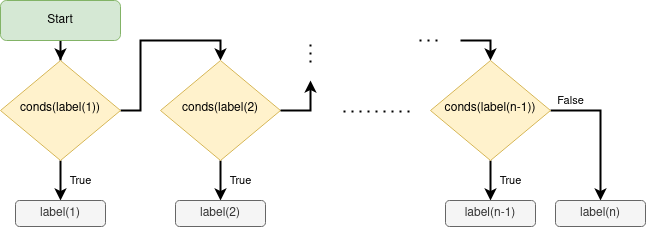
\includegraphics[width=\textwidth]{logic-based-classification/multi-label-selection.png}
\label{flowchart-multi-label-classification}
\end{figure}

The choice for the flowchart was made to aid interpretability because FastLAS learns the following set of rules:
\begin{verbatim}
conds(label(1)) :- ...
conds(label(1)) :- ...
...
conds(label(n-1)) :- ...
conds(label(n-1)) :- ...
\end{verbatim}
So, a human can easily determine the outcome by going through the rules from top to bottom and selecting a label matching the first satisfied rule.
Learning these types of rules is encoded in FastLAS with the following syntax:
\begin{verbatim}
#modeh(conds(const(learnable_label))).

... all the modeb declarations ...

% Avoid constraints
#bias("
:- constraint.
").
\end{verbatim}

Furthermore, to make the learner use the logic presented in the flowchart, we need to encode the following: 
\begin{enumerate}
    \item The position of a label in the flowchart chain.
    \item Selection the highest priority label whose conditions are satisfied.
    \item Selection of the lowest priority label when no conditions are satisfied.
\end{enumerate}
The enumerated criteria results in the following ASP encoding added to the background of a learning task:
\begin{lstlisting}
% Encoding 1 with label(name, position) (lower=better)
label(l1, 0).
label(l2, 1).
...
label(ln, n-1).

% Definitions of types for FastLAS
label(L) :- label(L, _).
learnable_label(L) :- exists_lower_priority(L, _).


% Encoding 2: Select the highest priority label whose conditions are satisfied
selected(L) :- label(L, P), conds(L), 
                 not higher_priority_selection(L, P).
higher_priority_selection(L, P) :- label(L, P), label(L2, P2), 
                                       P2 < P, selected(L2).

% Encoding 3: Select default label if no higher priority selection is made
selected(L) :- label(L, P), not higher_priority_selection(L, P), 
                 not exists_lower_priority(L, P).
exists_lower_priority(L, P) :- label(L, P), label(L2, P2), P2 > P.
\end{lstlisting}

Notice that the presented encoding also produces exactly one answer set, same as the encoding for the binary classification.

\begin{example}
Encoding the multi-label sudoku 4x4 learning task:

% INSERT reference evaluation
Consider an extension of the binary sudoku 4x4 task in example \ref{sudoku-binary-example}, which introduces an additional label \verb_conflict_. 
That label should be true only when an example contains two digit written in the same cell.
The following steps are needed to solve the task using the presented multi-label classification encoding:

1. \textit{Construct the background knowledge:} \\
The background is the same as for example \ref{sudoku-binary-example}.

2. \textit{Add the multi-label selection encoding to the background:} \\
We add the following rules to the background knowledge:
\begin{lstlisting}
% Encoding 1 with label(name, position) (lower=better)
label(conflict, 0).
label(invalid, 1).
label(valid, 2).

% Definitions of types for FastLAS
label(L) :- label(L, _).
learnable_label(L) :- exists_lower_priority(L, _).


% Encoding 2: Select the highest priority label whose conditions are satisfied
selected(L) :- label(L, P), conds(L), 
                 not higher_priority_selection(L, P).
higher_priority_selection(L, P) :- label(L, P), label(L2, P2), 
                                       P2 < P, selected(L2).

% Encoding 3: Select default label if no higher priority selection is made
selected(L) :- label(L, P), not higher_priority_selection(L, P), 
                 not exists_lower_priority(L, P).
exists_lower_priority(L, P) :- label(L, P), label(L2, P2), P2 > P.
\end{lstlisting}

2. \textit{Construct the language bias:} \\
We chose that we wish to learn what makes a cell invalid in this example, resulting in the following language bias:
\begin{verbatim}
#modeh(conds(const(learnable_label))).

#modeb(row(var(cell), var(row))).
#modeb(col(var(cell), var(col))).
#modeb(block(var(cell), var(block))).
#modeb(neq_cell(var(cell), var(cell))).
#modeb(value(var(cell), var(num))).

#maxv(4).
\end{verbatim}

4. \textit{Add examples and prior penalty definitions:}
% INSERT refernce to example definition and prior penalty definition
This step will be discussed in X and X.
\end{example}


\subsection{Creating the Example File}

The example file incorporates all of the theory presented in \ref{choosing-fastlas-parameter-values}.
% TODO: insert background example and write task name
Recall from X that the ILP-X task allow positive and negative examples.
Positive examples are bravely entailed, i.e. the final solution should be extended by at least one answer set.
On the other hand, the negative examples are cautiously entailed, so the final solution must not be extended by any answer set.
Because of our classification encodings, the learned hypothesis can only ever return one answer set, making the positive examples sufficient to encode any task.

To account for FastLAS's inability to deal with probabilistic atoms, we need to sample $I$ examples, each of the form:
\begin{lstlisting}
#pos(example_id@$\text{round} \left ( -\frac{K}{I} \ln \left ( \frac{\epsilon}{1 - \epsilon} \right ) \right )$,
{selected(true_label)},
{selected(incorrect_label) for each incorrect_label}, 
{... context atoms derived from the raw example ...}
\end{lstlisting}

The values for the constants $K, I,$ and $\epsilon$ are currently set to $1000, 100$ and $0.01$, respectively.

We further need to encode the prior (hypothesis) penalties.
% INSERT reference decomposable %
Any custom defined FastLAS scoring must be decomposable, and we can only directly input the scoring function decomposition as FastLAS code.
Recall that the scoring function decomposition we wish to encode is given by $\curly{S}^{rule}(r, T) = K \left (\ln (n_l - m_l) - \ln m_l  \right)$.  \\
% INSERT reference scoring function background which should include the simplest example.
As mentioned in X, defining a scoring function decomposition is done by defining the predicate \verb_penalty/2_. Any logic related to \verb_penalty/2_ is defined with atoms \verb+in_head/1+ and \verb+in_body/1+ which contain all the head and body predicates of a rule $r$.
Using FastLAS's ASP syntax, we define the \verb_penalty_ predicate by looking up the penalty value for a rule of a certain length, or assign an extremely large value for undefined length-penalty pairs:
\begin{lstlisting}
#bias("
penalty(P, custom) :- L = #count{X : in_head(X); X : in_body(X)}, 
                         pen(L, P).
pen(1, $K \ln (n_1 - m_1) - K \ln m_1$).
pen(2, $K \ln (n_2 - m_2) - K \ln m_2$).
... other similarly defined penalties ...
pen(L, 100000000000) :- L = #count{X : in_head(X); X : in_body(X)}, 
                           L >= threshold.
").
\end{lstlisting}


A simple, yet extremely beneficial, implemented optimisation is \textbf{example aggregation}. \\
When sampling $I$ values, track each outcome and the its number of occurrences before generating the actual examples.
The tracking allows to replace $C$ identical examples of penalty $\text{round} \left ( -\frac{K}{I} \ln \left ( \frac{\epsilon}{1 - \epsilon} \right ) \right )$ with only one example of penalty $C * \text{round} \left ( -\frac{K}{I} \ln \left ( \frac{\epsilon}{1 - \epsilon} \right ) \right )$, reducing the overall FastLAS running time.

% TODO: Example for binary sudoku with this one

% \subsubsection{Search Space Counting}
% TODO: Finish Implementation

\section{Evaluation}

The evaluation is carried out on two tasks: 
\begin{enumerate}
    \item Sudoku grid validity
    \item MLB-V2E classification
\end{enumerate}

The former is a much simpler task which will evaluate whether the method does indeed work well, while the latter will consider the Prob-FF-NSL framework within the context of a concept bottleneck pipeline.

\subsection{Sudoku grid learning}

This task aims to determine whether a sudoku grid with hand-written digits is valid, i.e. there are no repeated number in block, row nor column.
% INSERT FF-NSL
It is the repeat of the task studied in X.
There are two versions of it, 4x4 and 9x9 sudoku grid validity tasks.

The network uses a probabilistic ILP framework to account for uncertainties in the digit prediction NN.
The prediction confidence values are inputted to the Prob-FF-NSL framework.

Given that this task is simple to tackle for a logic-based learning system and a standard CNN, it is explored with different percentages of digit images are subject to a distribution shift.
The distribution shift in this case is a 90 degree image rotation.
It has a significant impact for the overall task, reducing the accuracy of digit prediction from 99\% to 14\%.

We will compare the our approach to three baselines: random forest, CNN-LSTM architecture and FF-NSL architecture. 
The latter similarly uses example penalties to give higher penalties to more likely examples, but the selection of the penalties was done through empirical evaluation.
% INSERT reference to section with FF-NSL
It is explained in more detail in X.
% INSERT Uncertainty-aware deep classifiers using generative models
The FF-NSL and Prob-FF-NSL are tested out with a standard digit predictor and uncertainty aware one based on X.
The standard digit predictor is often confidently wrong under a distribution shift, while the uncertainty aware one returns a more evenly spread out distribution upon seeing unfamiliar examples.

The learned models are compared with the true test set and the shifted test test.
The former always inputs the correct value to the network, while the latter has the same proportion of digit images shifted as the Prob-FF-NSL training set.

The results for the sudoku 4x4 task are shown in figure \ref{sudoku4x4-results}.

\begin{figure}[h]
\caption{A comparison of the sudoku 4x4 task performance with increasing level of distribution shifts}
\centering
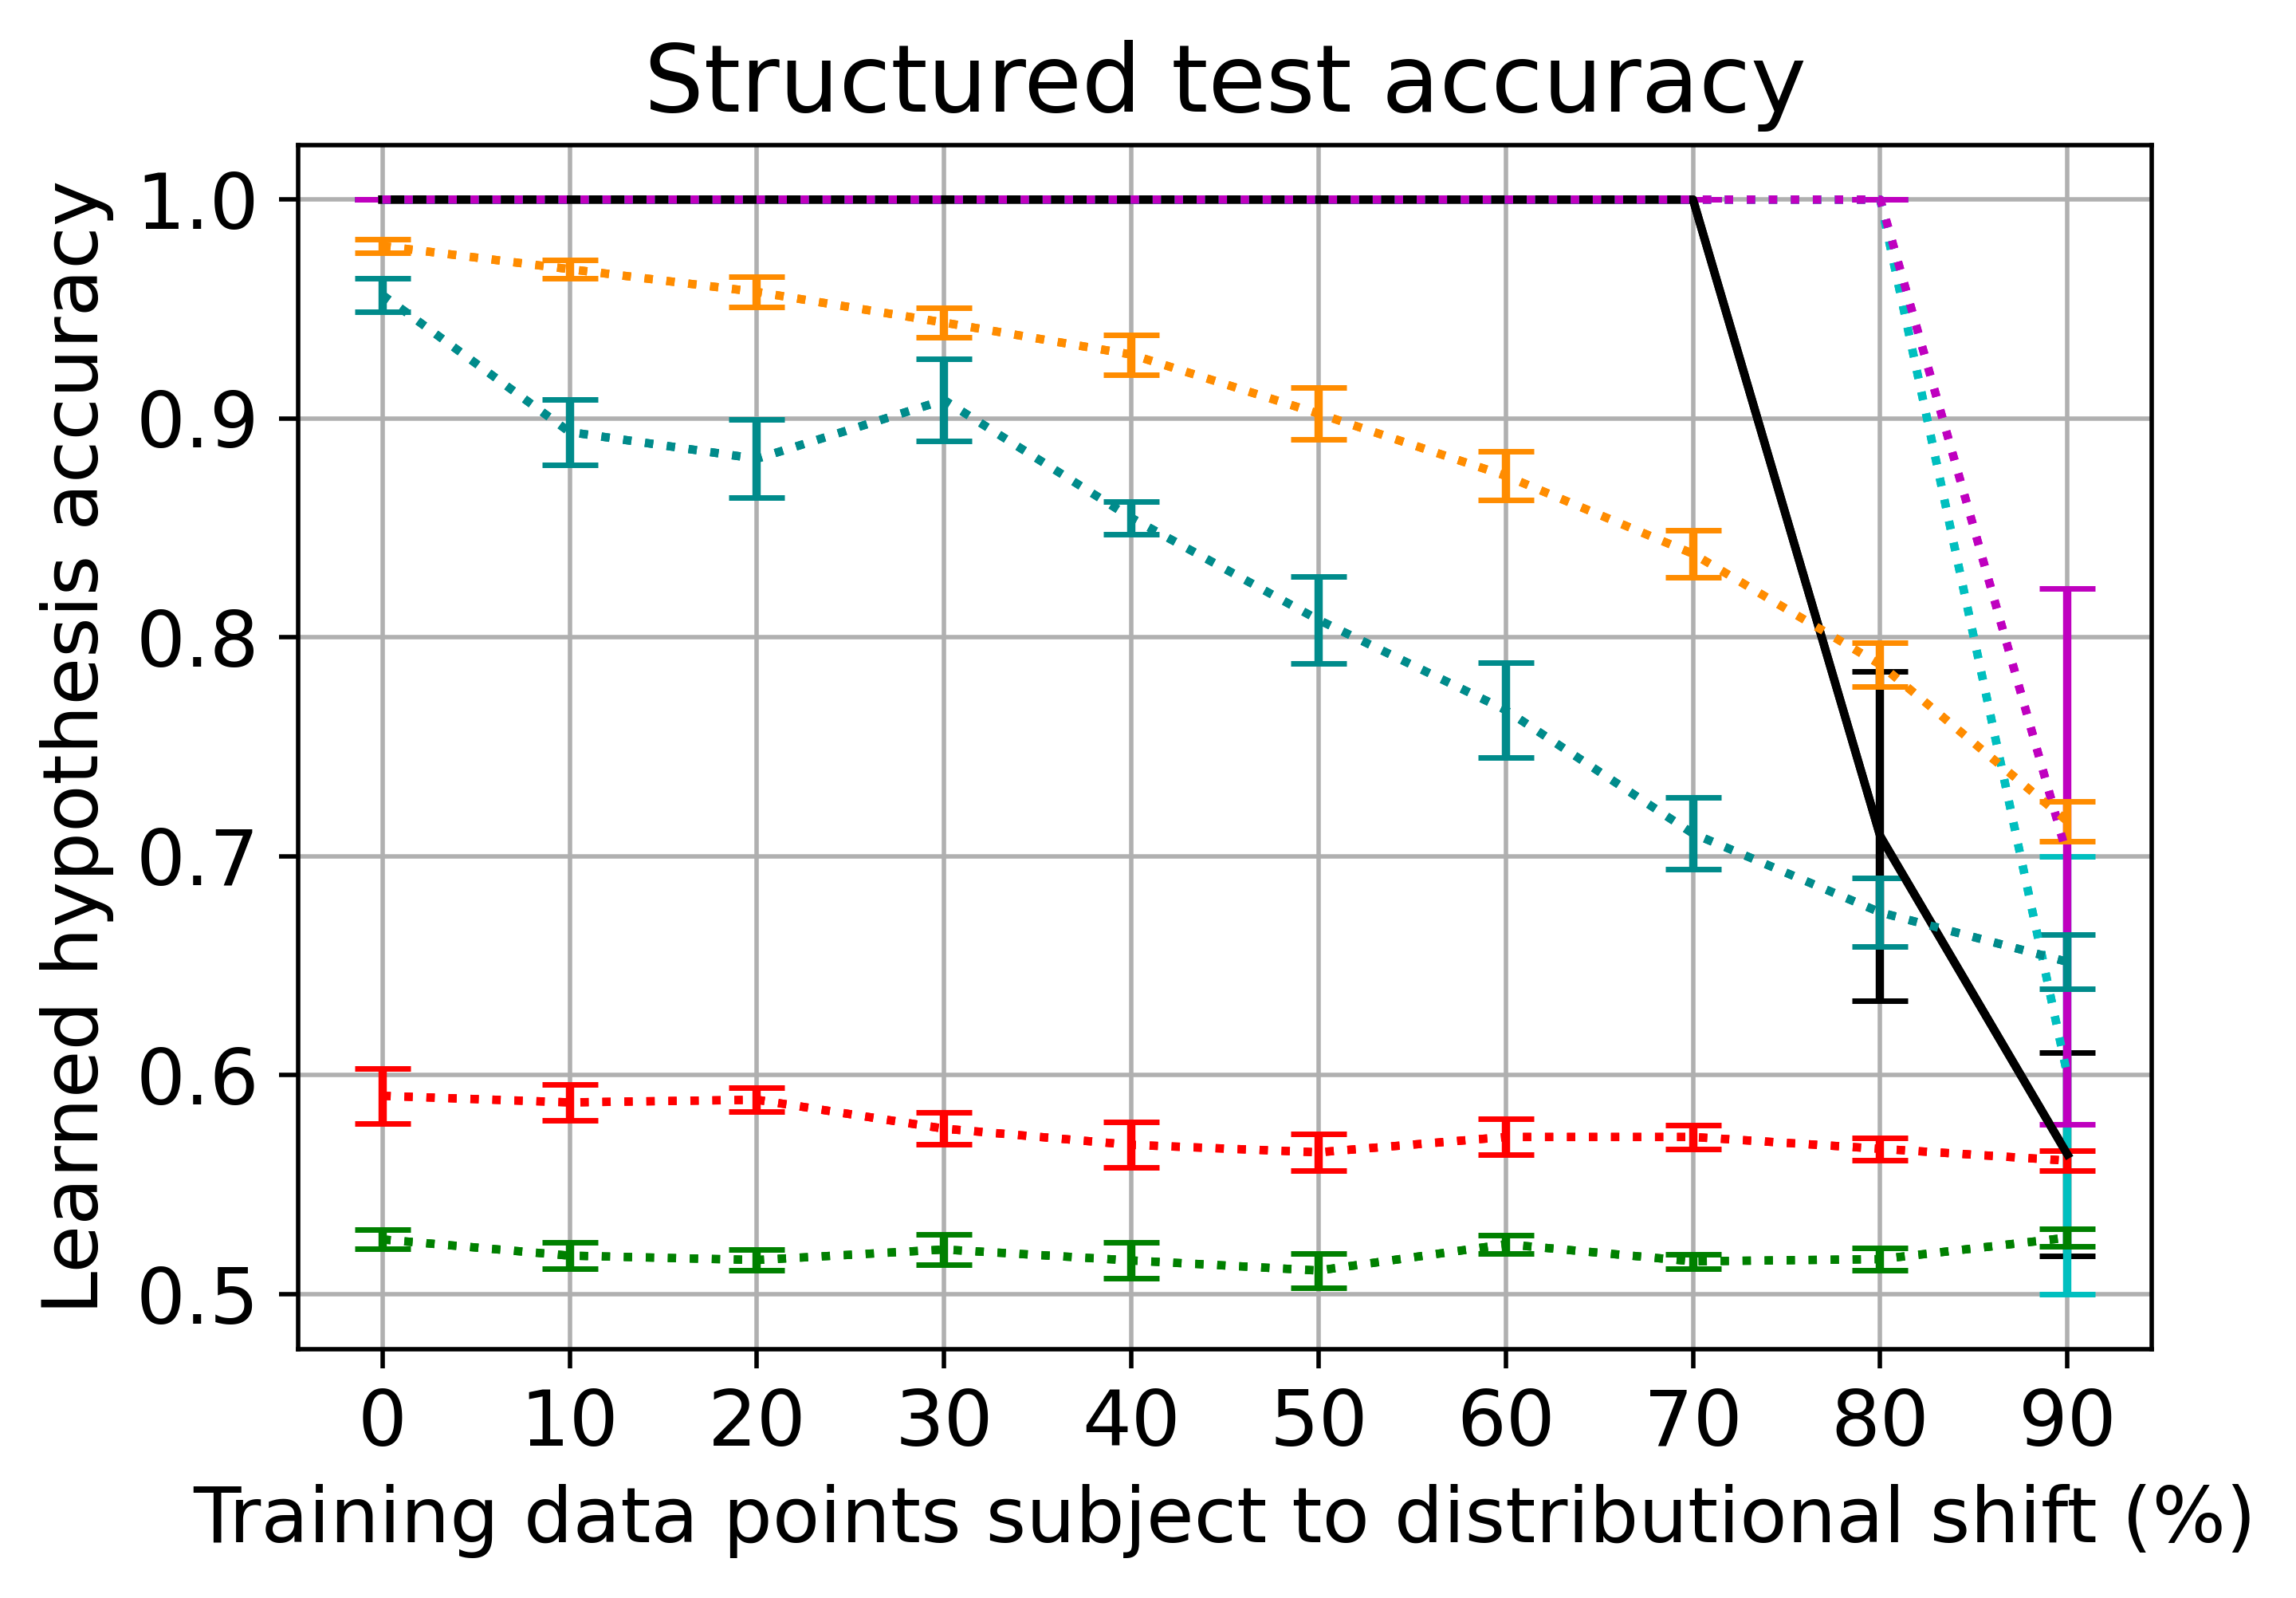
\includegraphics[width=\textwidth]{logic-based-classification/sudoku_4x4_structured_test_data_results.png}
\label{sudoku4x4-results}
\end{figure}



The results for sudoku 9x9 are shown in figure \ref{sudoku9x9-results}
\begin{figure}[h]
\caption{A comparison of the sudoku 4x4 task performance with increasing level of distribution shifts}
\centering
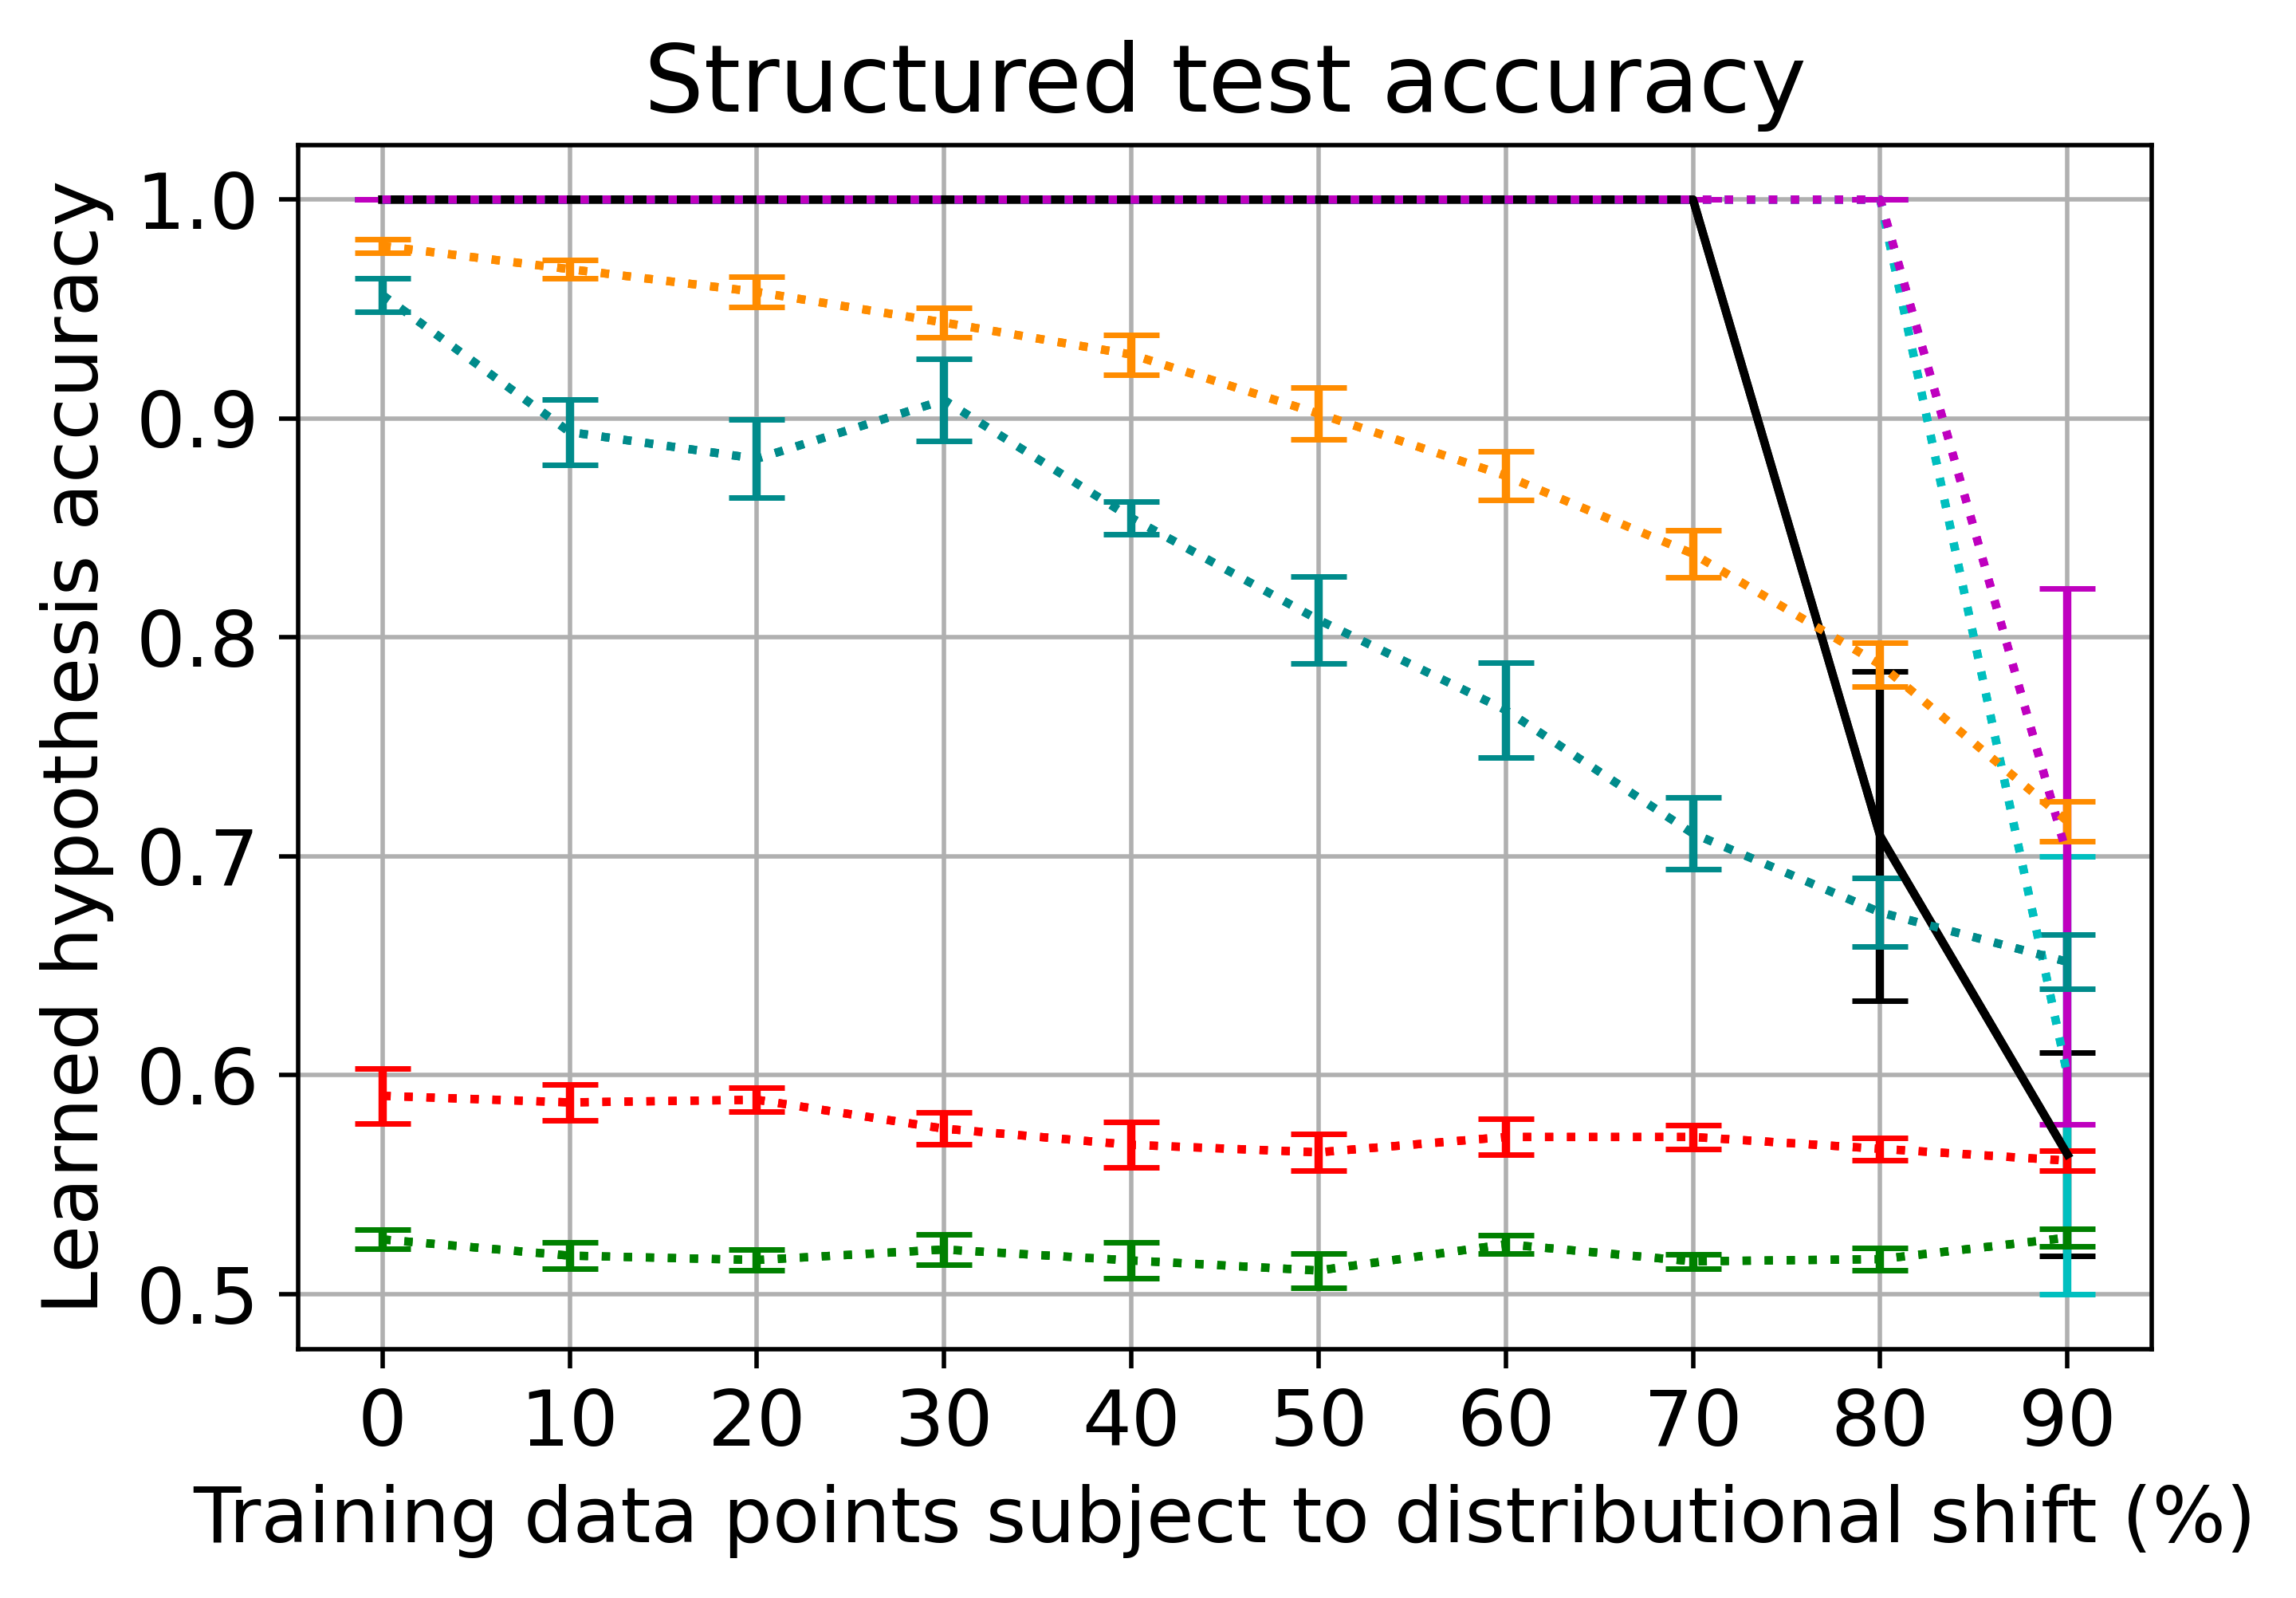
\includegraphics[width=\textwidth]{logic-based-classification/sudoku_4x4_structured_test_data_results.png}
\label{sudoku9x9-results}
\end{figure}


All in all, the Prob-FF-NSL generally performs well, having a perfect true test score in spite of 70\% of examples under a distribution shift.
However, it performs worse than the FF-NSL method on this particular task. 
The reason for it is the higher importance the FF-NSL assigns to the train examples that are not under the distribution shift.
It may be useful to integrate a similar notion of example importance to the Prob-NSL approach too.


\subsection{Concept Bottleneck Pipeline}

We also test the presented Prob-NSL framework within the context of a concept bottleneck model.
The architecture that the Prob-NSL model used for this task is presented in \ref{change-to-the-concept-bottleneck-architecture}.

As baselines, we compare the model to an end-to-end network and the concept bottleneck model with identical architectures.
The latter is the same model that is used for the concept prediction for the Prob-NSL model.

Their results are summarised in the table below:

\begin{center}
\begin{tabular}{ |M{3cm}||M{3cm}|M{3cm}|M{3cm}|  }
 \hline
 \multicolumn{4}{|c|}{Accuracy Comparison} \\
 \hline
 \hline
  & End-to-end model&Concept bottleneck model & Prob-NSL concept bottleneck \\ 
 \hline
 Train & X $\pm$ X & X $\pm$ X & 0.922 $\pm$ 0.021 \\
 Test & 0.687 $\pm$ 0.004 & 0.685 $\pm$ 0.005 & 0.910 $\pm$ 0.023 \\
 \hline
\end{tabular}
\end{center}

The Prob-NSL model greatly outperforms the other two with ~33\% test higher test set accuracy.
The results could have been even higher if there the concept bottleneck model is able to distinguish between \emph{strike} and \emph{ball} well.
In some instances, the model predicts a \emph{strike} in every case where there is a \emph{strike}.
When the model learns well enough to distinguish between the two, the accuracy jumps to values as high as 96\%.

\section{Discussion}

The proposed logic based classification method, working extremely well as a part of the concept bottleneck pipeline.
It outperforms the approach from Chapter \ref{concept-bottleneck-pipeline}.

% INSERT Online Symbolic Learning of Policies for Explainable Security reference
The method could be further improved, such as setting different penalties on examples that we care more about being satisfied.
Moreover, the approach for choosing a prior chosen may not be flexible enough for all possible applications.
Incorporating the configurable prior approach shown in X would have a lot of benefit for some applications.

% TODO: Luke feedback -random forest -feature importance - how often a predicate gets used to make a prediction 
\chapter{Related Work}

% TODO: Alessandra feedback: Check the task we are doing is a form of semantic entailment, if it is pick 1/2 paper explaining it.

\section{Video Classification}

Even though the work on video classification is not closely related to this thesis's contributions, it should serve as a performance benchmark of the entire system.

There are a few popular datasets for video classification out there, such as YouTube-8M \cite{RefWorks:RefID:10-abu-el-haija2016youtube-8m:} and Kinetics \cite{RefWorks:RefID:9-carreira2017quo}.
The YouTube-8M \cite{RefWorks:RefID:10-abu-el-haija2016youtube-8m:} is an extensive benchmark for general video classification with around 8 million clips and 4800 visual entities.
Mao et al. \cite{RefWorks:RefID:4-mao2019hierarchical} achieved very high performance on the YouTube-8M dataset using a deep convolutional graph neural network and a multi-level feature extractor.
Kinetics-700 \cite{RefWorks:RefID:14-carreira2019short} dataset is the latest version of the popular Kinetics dataset, which contains 700 human action classes and around 650000 video clips.
The top-performing model at the dataset has been designed by Yan et al. which uses Multiview Transformers for Video Recognition. 
The core idea of this approach is to input multiple different "views" of an input video into a transformer model to achieve better results.
This approach resulted in a model with an accuracy of 82.2\% on the Kinetics-700 dataset with the top-5 accuracy of 95.7\%.

YouTube-8M and Kinetics datasets are somewhat different to the dataset the majority of the project will address.
The MLB-V2E sequences look very similar, given that all of the sequences start with a pitcher throwing a ball.

A dataset much more closely related to our problem is the MLB-YouTube \cite{RefWorks:RefID:3-piergiovanni2018fine-grained} dataset.
The segmented video classification part of this dataset is the base for the MLB-V2E \cite{RefWorks:RefID:16-2021automatic} dataset which also includes crowd-sourced explanations. 
The MLB-YouTube dataset is quite different from the alternatives discussed in this section because the scene is very similar in all videos, only a single camera view is used, and the activity itself is only different because of the movement of one person.
The MLB-YouTube paper validates the InceptionV3 \cite{RefWorks:RefID:49-szegedy2016rethinking} and I3D \cite{RefWorks:RefID:9-carreira2017quo} networks performance on the constructed datasets shown in the table below.
These results should serve as a guide for the results of this project.

\begin{center}
\begin{tabular}{ |p{2cm}|p{1cm} p{1cm} p{1cm} p{1cm} p{1cm} p{1cm} p{1cm} p{1cm}|  }
 \hline
 \multicolumn{9}{|c|}{Per-class average precision for the multi-class baseball classification} \\
 \hline
 Method & Ball & Strike & Swing & Hit & Foul & In Play & Bunt & Hit by Pitch \\
 \hline
 Random & 21.8 & 28.6 & 37.4 & 20.9 & 11.4 & 10.3 & 1.1 & 4.5 \\
 InceptionV3 & 66.9 & 93.9 & 90.3 & 90.9 & 60.7 & 89.7 & 12.4 & 29.2 \\
 I3D & 62.5 & 91.3 & 88.5 & 86.5 & 47.3 & 75.9 & 16.2 & 21.0 \\
 \hline
 
\end{tabular}
\label{inclusion-exclusion-rules}
\end{center}


\section{Definition of Concept in Other Settings}

There are different angles to the definition of concepts in various works.
As mentioned, this project defines a concept as a syntactic generalisation of an atomic sentence.
However, this approach is not common in other works which do concept extraction.


Formal concept analysis \cite{RefWorks:RefID:31-ganter2012formal} is a method for knowledge representation based on the lattice theory which can be used to extract hierarchical concepts.
It defines two fundamental notions: a formal context and a formal concept. 
Formal context K := (G, M, I) consists of a set of objects G, set of attributes M and relation I on (G, M).
If (g, m) $\in$ I, object g has attribute m.
Using these attributes, set A$' $ is defined containing all attributes common to the objects in a set of objects A.
Additionally, set B$' $ contains objects that have all attributes in the set of relations B.
From these definitions, formal concept of context (G, M, I) is defined as a pair (A, B) such that A $\subseteq$ G, B $\subseteq$ M, B$' $ = A and A$' $ = B.

The Formal Concept Analysis with text analysis is mainly used to construct the concept hierarchy, where a concept refers to a phrase containing two words.

For example, work by Cimiano et al. \cite{RefWorks:RefID:32-cimiano2005learning} extracts verb/subject, verb/object/ and verb/prepositional phrase as candidate concepts.
Moreover, the Formal Concept Analysis is used by Anoop et al. \cite{RefWorks:RefID:33-anoop2019extracting} to extract concepts with their relationships from unstructured text.
The authors manually extract stemmed noun phrases as key phrases and use indications such as "is-a" to generate a formal context table.
This table is then used to extract hierarchical concepts.

On the other hand, TaxoLearn \cite{RefWorks:RefID:34-dietz2012taxolearn} by Dietz et al. does not use Formal Concept Analysis but also extracts noun phrases as concepts. The relevance of noun phrases is checked by computing how often they appear in a particular context compared to other contexts. It also uses a hierarchical clustering algorithm to construct a taxonomy.

Moreover, approaches such as the one by Koh et al. \cite{RefWorks:RefID:35-koh2020concept} define concepts as properties that the image may have. These properties need to be provided beforehand.

Finally, work such as the one by Fan et al. \cite{RefWorks:RefID:50-fan2004semantic} use expert defined terms, such as \emph{Lecture Presentation for Gastrointestinal Surgery}, as semantic concepts. 


\section{Concept-Based Explanations for Images and Text}

Concept-based explanations for images and text attempts is a more straightforward related problem.
Koh et al. \cite{RefWorks:RefID:35-koh2020concept} predict a set of pre-labelled concepts which they use to make a final classification.
The pipeline by Koh et al. is similar to the pipeline that will be used in this project, just that the concepts are automatically extracted instead of provided.
Yeh et al. \cite{RefWorks:RefID:36-yeh2019completeness-aware} propose a method that automatically extracts sets of pixels from an image that represent valuable concepts.
Similarly, Ghorbani et al. \cite{RefWorks:RefID:37-ghorbani2019automatic} propose another method that automatically extracts a set of visual concepts which are meaningful to humans.
All outlined methods are based on visual concept extraction, unlike this project's concept extraction, which will mainly focus on the events/actions in the baseball video sequence.


\section{Video Explanation}

Another related problem is that of Video Explanations. This project may even explore it at a later stage within the context of a concept extraction pipeline.

One famous dataset for video understanding is the MSR-VTT dataset \cite{RefWorks:RefID:40-jun2016msr-vtt:}. It is a large scale dataset with more than 10000 video clips in 257 popular categories of a video search engine.
Each video is annotated with roughly 20 sentences. 
A few different approaches for tackling this issue are presented as viable options in the paper, such as 2D Convolutions, 3D Convolutions, and RNNs.
One of the most performant methods on this dataset is CLIP2TV \cite{RefWorks:RefID:41-gao2021clip2tv:}, which utilises transformer-based techniques for both video and text representation.


The authors of the MLB-V2E \cite{RefWorks:RefID:16-2021automatic} have also constructed the MSR-V2E \cite{RefWorks:RefID:16-2021automatic} dataset, which uses the clips made available by the MSR-VTT and provides new classification labels and explanations.
This dataset will likely be used for the evaluation of this project.

\section{Semantic Concept Video Classification}

Semantic Concept Video Classification attempts to predict a set of predefined concepts from a video.
Predicting a set of predefined concepts from a video is closely related to a part of the pipeline in this project, which indicates which extracted concepts occur before predicting the outcome. 

The work by Fan et al. \cite{RefWorks:RefID:50-fan2004semantic} tries to predict semantically defined concepts by medical experts.
The paper proposes using salient objects, which are visually-distinguishable video components that human semantics understands, to model these semantical concepts.
Examples of notions salient objects attempt to represent are a face, voice, or a lecture slide.
Despite its benefits, the semantics of salient objects is quite simple, and it does not model relationships that happen over multiple frames in a video.
Newer work by Fan et al. \cite{RefWorks:RefID:51-jianping2007incorporating} also incorporates the possibility of a hierarchical concept classification. The approach also predicts atomic video concepts before constructing the higher-level ones and existing concept ontology.

Assari et al. \cite{RefWorks:RefID:52-assari2014video} represent a video by the co-occurrence of the semantic concepts before applying a classifier.
The concepts in this work are also predefined, but they represent a set of events rather than a set of objects.



% Luke feedback: Wee need to handle that more general concepts are often much more frequent then it is described 
% For example - bird has feathers should exist in all cases but it is only described when the feathers are special.

\chapter{Conclusion}

This paper demonstrates that a concept bottleneck model can be combined with human-generated explanations to improve NN explainability.
In doing so, we have discovered the following findings:
\begin{enumerate}
    \item \textbf{Logic-based methods can effectively be used to tackle some NLP seq2seq problems}.
    Such an approach was crucial as the datasets were tiny, consisting of only around 100 examples per problem.
    The dataset size made it impossible to use state-of-the-art NLP techniques such as transformers.
    On the other hand, the solutions made by hand-crafting or learning a set of rules could achieve good performance despite the dataset size.
    However, the limitation is the lack of scalability of the underlying ILASP \cite{RefWorks:RefID:54-ilasp} system used to learn a set of rules.
    It was applied successfully on the generalisation task, while it was far off its theoretical optimality guarantee for the atomisation task.
    When we applied it successfully, it did produce a better solution than a hand-crafted set of rules.
    
    
    \item \textbf{The newly proposed CoDEx pipeline significantly outperforms its predecessor}. 
    We have replaced the extraction part of the original pipeline with the new atomisation and generalisation stages.
    A new set of concepts is much more informable and better at predicting the final label.
    There is also an indication that the concepts it produced are better, but a large-scale human study must be conducted to validate such results.
    However, the CoDEx module still has room for improvement, as it cannot account for concepts occurring in the video but not explicitly in the explanation.
    This limitation leads to poor concept precision values.
    In addition, the limitation makes applying the sequential training procedure challenging, which splits the training of concept and label prediction parts of the network.
    Sequential training would be preferred, given that the joint training may not truly use concepts to predict the results.
    We further show that the CoDEx pipelines, although well performing, do not extract a valuable set of concepts given a set of general image descriptions.
    So, the applicability scope of this method needs to be further investigated. 
    But, we believe it should work for any domain where the human-generated explanation is written to describe the final label.
    
    \item \textbf{The proposed logic-based classification produces high-performing and easily explainable solutions}.
    We show that the method can be applied to the concept bottleneck pipeline exceptionally well.
    It helped achieve much better results for the MLB-V2E dataset \cite{RefWorks:RefID:16-2021automatic} compared to the original concept-bottleneck models while being completely interpretable.
\end{enumerate}

\section{Future work}

There are several directions possible to take this project further. We highlight some of the ideas for doing so in this section. \\

The most pressing concern is the CoDEx sparsity.
The human-generated explanations do not capture all of the concepts present in the concept matrix explicitly.
For example, both \emph{The ball was caught by the outfielder} and \emph{The outfielder got the pitch} would be extracted as separate concepts.
These sentences could have been grouped with some combination of hyper-parameters. 
However, finding such values often had an undesirable knock-on effect.
For example, \emph{The ball was outside of the strike zone} and \emph{The ball was inside of the strike zone} would almost always be grouped before the first two sentences are. \\
% INSERT An Inference Model for Semantic Entailment in Natural Language
To mitigate that issue, we might use models that solve the semantic entailment problem.
The semantic entailment task aims to determine whether some sentence S could be inferred by a sentence T.
Such information would allow us to group \emph{The ball was caught by the outfielder} and \emph{The outfielder caught the pitch} seamlessly.


Another possible direction could involve improving upon the video classification network.
We could enhance the current neural network architecture.
% INSERT Deep residual learning for image recognition
It consists of image features extracted by ResNet, from which motion features are captured using 1D convolution.
Much better architectures do exist, such as the ones discussed in \ref{video-classification}.
We expect that an improved architecture should improve concept prediction performance, which in turn improves the final class prediction.

Comparing the performance with the original concept bottleneck \cite{RefWorks:RefID:35-koh2020concept} would also be beneficial.
This work extends upon the original idea by mining the concepts from explanations.
% INSERT The caltech-ucsd birds-200-2011 dataset
The original work uses a human-engineered set of valuable concepts, which they applied to the CUB-birds dataset (X).
Comparing with the same dataset would give more insight into the generality of the concepts extracted by the CoDEx pipeline.


Moreover, the concept explanation quality should be evaluated using a human study, such as a Mechanical Turk analogous to \cite{RefWorks:RefID:16-2021automatic}.
Such a study would give more confidence regarding the quality of generated explanation.
In addition, we should also construct a human study interpreting the logic-based classification framework.

Finally, we could improve upon the atomisation procedure.
The atomisation procedure is the main culprit behind any concepts that are invalid sentences.
With the Jaccard score at around 0.5, the atomisation task has a lot of room for improvement. \\
% INSERT reference Exploring the limits of transfer learning with a unified text-to-text transformer.
A possible approach for handling this issue may involve trying to solve this problem using a seq2seq transformer such as T5.
It would require greatly extending the existing dataset, but it would undoubtedly perform better with a sufficient number of examples.

\appendix
\chapter{Ethics}

The following section is based on the ethics checklist provided by the Computing Department. 
The checklist consists of a series of yes/no questions. 
If an answer was yes, there is an ethical issue that needs to be considered.
These answers will form a basis for the discussion in this chapter. \\


\emph{"Does the project involve human participants?"}
The project will involve human participants in two ways: 

    - For result validation. Some results obtained in the project have been obtained with human participants, e.g. generated explanation correctness.
    
    - For dataset construction. The datasets used for this project, MLB-V2E \cite{RefWorks:RefID:16-2021automatic} and MSR-V2E \cite{RefWorks:RefID:16-2021automatic}, used human-generated explanations.

Both cases are not harmful to anyone involved. The only care that needs to be taken is regarding the personal information of the subjects involved, which is discussed in the following question.
Additionally, the participants involved in the dataset construction were compensated 15\$ per hour, as discussed in the paper under review \cite{RefWorks:RefID:16-2021automatic}.\\

\emph{"Does your project involve personal data collection and/or processing?"}

The dataset construction required subjects to explain a video in their own words.
But, this data is entirely anonymous and cannot be de-anonymised.
No explanation that is provided is in any way, shape or form personally identifiable information so that it can be linked back to a specific person.

Any data acquired from new participants during this project will be fully anonymised as well. \\

\emph{Will your project use or produce software for which there is a copyrighting licensing implication?}
The project uses three different, third-party pieces of software.
These are \emph{spacy} \cite{RefWorks:RefID:24-spacy}, \emph{FastLAS} \cite{RefWorks:RefID:19-law2020fastlas:}, \emph{ILASP} \cite{RefWorks:RefID:18-law2020ilasp}, and \emph{clingo} \cite{RefWorks:RefID:22-clingo}.
\emph{FastLAS}, \emph{spacy} and \emph{clingo} use the MIT License \cite{RefWorks:RefID:53-mit}.
The MIT License is a permissive license that does not block any future publication and only requires the preservation of copyright and license notices.
On the other hand, \emph{ILASP} is free for use for university research, but it will require reaching out to Mark Law for commercial purposes \cite{RefWorks:RefID:54-ilasp}.
The licenses are not an issue as it stands. \\


To sum up, this project has no outstanding ethical issues which need to be resolved.

\chapter{Concept Bottleneck Model}
\label{concept-bottleneck-architectures}

This appendix presents networks used in Chapter \ref{concept-bottleneck-pipeline}.
In order to reproduce the results similar to this project, one needs to train them for 100 epochs, using the adam optimiser, and the batch size of 32. \\
The number next to layer name, such as \verb_5 Dense_, represents the number of outputs of that layer.
The network for the MLB-V2E dataset is shown in \ref{mlb-network-1} and \ref{mlb-network-2}, while the bird-flowers datset network is in \ref{birds-flowers-network}.

\begin{figure}[h]
\caption{MLB-V2E baseball network part 1}
\vspace{10pt}
\centering
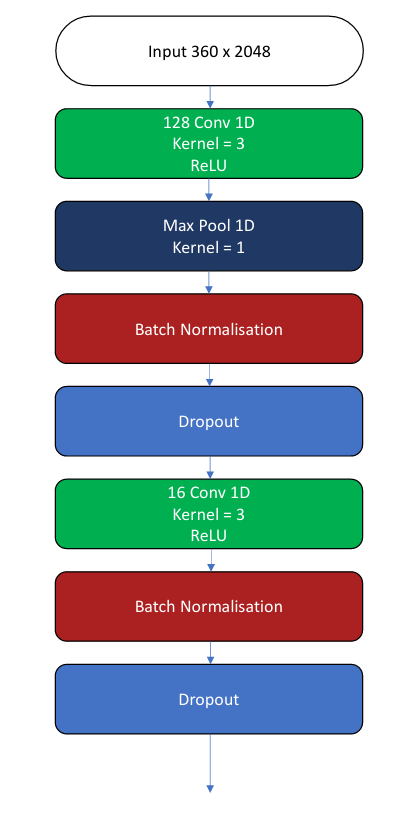
\includegraphics[width=0.6\textwidth]{appendix/mlb-network part 1.png}
\label{mlb-network-1}
\end{figure}

\begin{figure}[h]
\caption{MLB-V2E baseball network part 1}
\vspace{10pt}
\centering
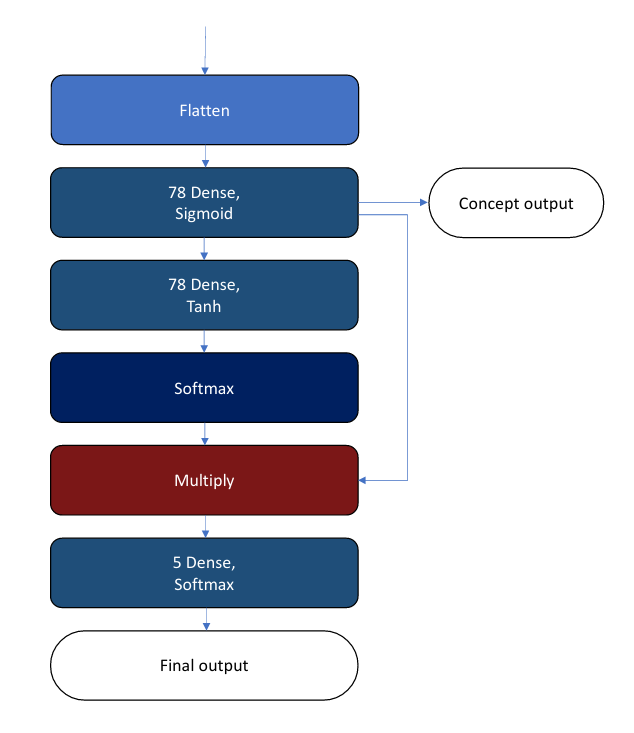
\includegraphics[width=\textwidth]{appendix/mlb network part 2.png}
\label{mlb-network-2}
\end{figure}

\begin{figure}[h]
\caption{MLB-V2E baseball network part 1}
\vspace{10pt}
\centering
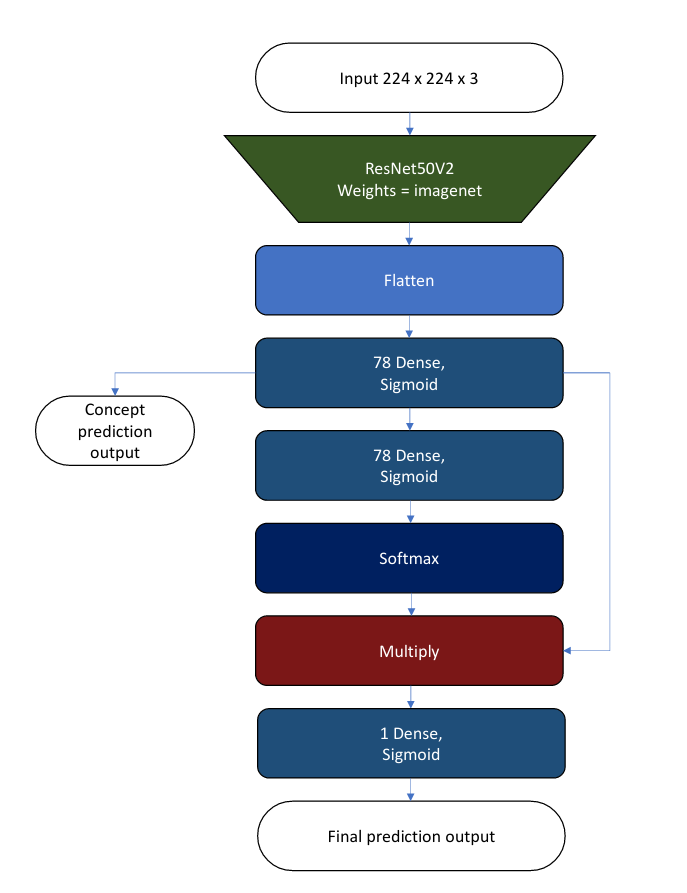
\includegraphics[width=\textwidth]{appendix/birds flowers prediction network.png}
\label{birds-flowers-network}
\end{figure}



%\bibliographystyle{alpha}
%\bibliography{bibs/sample}

%\bibliographystyle{plainnat}
%\bibliography{bibs/export.bib}

\printbibliography

\end{document}